%!TEX program = xelatex
% Copyright (C) 2018 by latexstudio <http://www.latexstudio.net>
%
% This program is free software: you can redistribute it and/or modify
% it under the terms of the GNU General Public License as published by
% the Free Software Foundation, either version 3 of the License, or
% (at your option) any later version.
%
% This program is distributed in the hope that it will be useful,
% but WITHOUT ANY WARRANTY; without even the implied warranty of
% MERCHANTABILITY or FITNESS FOR A PARTICULAR PURPOSE.  See the
% GNU General Public License for more details.
%
% You should have received a copy of the GNU General Public License
% along with this program.  If not, see <http://www.gnu.org/licenses/>.
%

%\documentclass{ctexart}
%
%\setCJKmainfont{Source Han Sans SC}
%  %[
%  %  UprightFont    = * Medium,
%  %  BoldFont       = * Bold,
%  %  ItalicFont     = * Medium,
%  %  BoldItalicFont = * Bold
%  %]
%\begin{document}
%你好,世界
%
%\end{document}

\documentclass{latex-faq-cn-class}
% 如果遇到字体问题,可以选择不使用自定义字体:
% \documentclass[use-customized-fonts=false]{latex-faq-cn-class}

\usepackage{dirtree}
\usepackage{graphicx}

% TODO: 移植到 class
% \makeatletter
% \def\@captype{figure}
% \makeatother

\title{\LaTeX{} 常见问题}
\author{\LaTeX{} Studio 团队}

\begin{document}

\maketitle

% \def\FONTTEST{字体测试骨头 ABC fi fl\ }
% \FONTTEST \textit{\FONTTEST} \textbf{\FONTTEST \textit{\FONTTEST}}          \par
% \textsf{\FONTTEST \textit{\FONTTEST} \textbf{\FONTTEST \textit{\FONTTEST}}} \par
% \texttt{\FONTTEST \textit{\FONTTEST} \textbf{\FONTTEST \textit{\FONTTEST}}}

% Copyright (C) 2018 by latexstudio <http://www.latexstudio.net>
%
% This program is free software: you can redistribute it and/or modify
% it under the terms of the GNU General Public License as published by
% the Free Software Foundation, either version 3 of the License, or
% (at your option) any later version.
%
% This program is distributed in the hope that it will be useful,
% but WITHOUT ANY WARRANTY; without even the implied warranty of
% MERCHANTABILITY or FITNESS FOR A PARTICULAR PURPOSE.  See the
% GNU General Public License for more details.
%
% You should have received a copy of the GNU General Public License
% along with this program.  If not, see <http://www.gnu.org/licenses/>.
%

\section{最常出现的问题}
\label{sec:starter}

\faq{论文 / 比赛的 deadline 要到了,如何在一天 / 两天 / 三天之内入门 \LaTeX{}?}{get-started}

非常遗憾,这几乎是不可能完成的任务。在时间紧张、压力巨大的情形下,入门 \LaTeX{} 对您来说没有意义。
作为排版工具,\LaTeX{} 实现的效果远没有文章的内容重要,所以请不要在这种情况下把您的精力投入在学习
\LaTeX{} 上。

通常来说,我们建议您至少通过三个月的时间来入门 \LaTeX{},并在之后的工作、学习中不断深入理解、
积累经验。

如果确有必要在短时间内掌握 \LaTeX{} 的使用方法,请联系靠谱且有经验的人。注:很多“学长”、“老师”都是
不靠谱的,所以这一点实际上很难办到。


\faq{如何“安装 \LaTeX{}”?}{install-latex}

如果您也有这一问题,首先需要澄清一些概念,见~\faqref{tex-terms}。简短来说,\LaTeX{} 本身是一种标记
语言,而不是 Microsoft Word 一样现成的软件。因此,社区将相关的支持文件、可执行程序、文档等打包在了
一起,形成了可供用户下载、安装的发行版(distribution)。一般而言,“安装 \LaTeX{}”指的就是安装
发行版。

目前,根据平台不同,可供使用的主流发行版有以下这些:

\begin{itemize}
  \item \TeXLive{},见~\faqref{install-texlive}
  \item \MiKTeX{},见~\faqref{install-miktex}
  \item \MacTeX{},适用于 macOS,见~\faqref{install-mactex}
  % TODO: 更多的发行版介绍
  \item 【有待整理】
\end{itemize}


\faq{我的 \CTeX{} 为什么……}{why-ctex}

您在这里提到的“\CTeX{}”,指的很可能是由中国 \TeX{} 社区(即 \CTeX{} 社区)所发布的、以 \MiKTeX{}
为基础的一个发行版,全称为“\href{http://www.ctex.org/CTeX}{\CTeX{} 套装}”。这一发行版目前已停止
维护,所以除非必要,请不要再使用。\TeXLive{} 以及 \MiKTeX{} 都是可靠的替代方案。

\CTeX{} 社区另发布了一个同样称为 \href{https://www.ctan.org/pkg/ctex}{\CTeX{} 的宏集}(宏包),
这是目前在 \LaTeX{} 中使用中文排版的推荐方案。如果您需要获取相关信息,请查阅其文档。\CTeX{} 宏集
的有关问题,在本文之后也有涉及。

\section{背景知识与基本概念}

\begin{faq}{什么是 \TeX{}?}
\TeX{} 是由著名计算机科学家 Donald~E. Knuth(高德纳)发明的排版系统。他在《The \TeX book》一书的
前言中曾提到:“(\TeX{})旨在创造美丽的书籍,尤其是那些包含很多数学公式的书。”
\footnote{原文如下:“This is a handbook about \TeX{}, a new typesetting system intended for the
creation of beautiful books---and especially for books that contain a lot of mathematics.”}

1976 年,Knuth 出版鸿篇巨著《The Art of Computer Programming》第二卷的第二版,但当时所用的照排技术
却令他非常失望。作为斯坦福大学计算机科学系的教授,Knuth 决定自己开发一套高质量的排版系统。1978 年,
他开发出了 \TeX{} 的第一个版本;随后,又在 1982 年推出了 \TeX{} 的第二个版本(\TeX 82),也就是
人们今天所用 \TeX{} 的基础。Knuth 将 \TeX{} 的源代码无偿发布在公有领域
\footnote{\TeX{} 使用的许可证为 \href{https://www.ctan.org/license/knuth}{Knuth License}。},
这使得他人可以进一步完善这一系统,并增加新的功能。

在今天,\TeX{} 既可以指 Knuth 发明的这一套排版系统,也可以指相应的排版语言,有时候也指将其打包、
整理以方便用户使用的软件套装(发行版)。

\begin{reference}
  \item https://texfaq.org/FAQ-whatTeX
  \item \TeX{}, Wikipedia, The Free Encyclopedia, \url{https://en.wikipedia.org/wiki/TeX}
\end{reference}

% Knuth 是美国加州斯坦福大学计算机编程专业的名誉教授,他在 1978 年开发了第一个版本的 \TeX{} 用来处理
% 他的《计算机编程艺术》的修订。这个想法特别受欢迎,所以1982年他推出了 \TeX{} 的第二个版本,也就是
% 人们今天所用的 \TeX{} 的基础。
%
% Knuth 开发了一套“文学编程”系统来编写 \TeX{},他还提供了免费的 \TeX{} 资源,以及可以将网络
% 资源转化为可以编译或者打印的东西的工具;Knuth 做了什么,对人们来说从来都不是什么神秘的事情。
% \TeX{} 以及它的文档都是高度可移植的。
%
% 对于感兴趣的程序员来说,\TeX{} 有其迷人之处:没有什么能比得上一个人可以构建这样一个程序,至今它的
% 持续时间比大多数的程序都好,而且已经被移植到了许多不同的计算机构架和操作系统中许多现代编程所追求
% 的属性。经过处理的“可读”的 \TeX{} 程序源代码可以在 TDS structured 版本中找到。

% 来源 https://texfaq.org/FAQ-whatTeX
\end{faq}

\begin{faq}{什么是 \LaTeX{}?}
\end{faq}

\begin{faq}{\TeX{} 中常见术语的解释}
\textbf{引擎}
  
\LaTeX/\TeX{}解析引擎,其实就是一个编译器,它输入一个\verb|.tex|文件作为输入,根据源文件的内容送入解析引擎和渲染引擎进行处理,并将排版的成果——文档编译输出,\LaTeX/\TeX{}的解析引擎目前有pdflatex、xelatex、lualatex等,它们都可以输出pdf文档文件(部分解析器可以输出dvi文件),用于在多平台进行分发甚至打印出版。

\textbf{格式}

\TeX{} 是存在各种不同的封装格式的,比如原生的 \TeX{} 或者 \LaTeX{},我们所使用的 \LaTeX{} 只是\TeX{} 封装格式的其中一种,是目前流行的封装规范。

\textbf{发行版}

\LaTeX/\TeX{}都包含了成千上万个宏包,甚至有可能我们需要安装新的宏包,除了手动安装外,最好的方式就是利用发行版的宏包管理器,所谓发行版就是把\LaTeX/\TeX{}的相关组件打包,形成一个独立完善的\LaTeX/\TeX{}系统,目前流行的发行版有MiKTeX、proTeXt 以及TeXLive。
\end{faq}


\begin{faq}{}

\end{faq}

\begin{faq}{\LaTeX{} 源文件有什么要求?}
LaTeX的源文件是 *.tex文件,是指latex编译器处理输入文件的源码,latex编译器会对输入文件进行解析,构造解析树,进行渲染,然后输出处理后的文档,完成一次编译过程,由于LaTeX解析器可能对中文文件名处理存在兼容性问题,不建议将LaTeX的源文件的文件名设置为中文。
\end{faq}

\DeclareRobustCommand\cs[1]{\texttt{\char`\\#1}}
\providecommand\marg[1]{\texttt{\{<#1>\}}}
\providecommand\oarg[1]{\texttt{[<#1>]}}
\providecommand\Arg[1]{\texttt{\{#1\}}}
\providecommand\env{\texttt}
\providecommand\pkg{\textsf}
\providecommand\cls{\textsf}
\providecommand\file{\textsf}



\section{安装与配置问题}

\begin{faq}{如何安装 LaTeX}

很多用户所谓的如何安装 LaTeX,实际上是一个无解的问题,因为 LaTeX
不是一款软件,相关概念不再赘述。用户可以直接安装 LaTeX 发行版,如
proTeXt , TeXLive 和 MacTeX (TeXLive在MacOS 的一个再次发行版)。
\end{faq}


\begin{faq}{如何下载 proTeXt 安装包}

访问以下链接即可
\url{http://mirror.ctan.org/systems/protext/protext.exe}
\end{faq}


\begin{faq}{如何下载 TeXlive 安装包}

访问以下网址获取 texlive 安装包镜像文件:
\url{http://mirror.ctan.org/systems/texlive/Images/texlive.iso}
MacTeX安装包下载地址:
\url{http://mirror.ctan.org/systems/mac/mactex/MacTeX.pkg}
\end{faq}


\begin{faq}{如何安装 TeXlive}

TeXlive 为用户提供了官方安装手册,其中文版地址是:
\url{https://tug.org/texlive/doc/texlive-zh-cn/texlive-zh-cn.pdf}
建议有余力的用户通读手册,以了解更多内容。

也可以参照以下网址 \url{https://www.tug.org/texlive/quickinstall.html}
\end{faq}


\begin{faq}{如何挂载镜像文件:}

目前市面上有很多虚拟光驱软件可供用户选择,例如 UltraISO。

特别一提,在 windows 8、windows 10
操作系统中,默认被双击后,镜像文件将会直接挂载。

在 Linux 操作系统中,可使用命令行挂载镜像文件:

\begin{verbatim}
mount -o loop ~/Download/TeXlive.iso ~/iso
\end{verbatim}
\end{faq}


\begin{faq}{挂载镜像文件后该如何做?}

windows 用户可以双击 install-tl-windows.bat 文件来进行安装。

linux 用户请在命令行执行 ./install-tl 进入 no gui 安装模式
\end{faq}


\begin{faq}{双击 install-tl-windows.bat 出现错误怎么办?}

使用命令行。同时按下 win 键和 R
键,打开``运行''窗口,在窗口的``打开''处,输入 cmd
打开命令行窗口(黑窗)。

在黑窗内输入

\begin{verbatim}
cd /d [~]
\end{verbatim}

后按 enter 键(即执行该命令),此处 {[}\textasciitilde{}{]} 代指
install-tl-windows.bat 所在目录,例如 C:/Downloads
等,注意命令中的空格。

进入目录后继续执行

\begin{verbatim}
install-tl-windows.bat -no-gui
\end{verbatim}

开启纯命令行安装模式。默认状态下,点击 I 键 ( HIJK 的
I),安装便会开始。若用户想改变安装路径或其他设置,只需根据屏幕提示进行更改即可。特别强调,安装路径一定是不带空格的纯英文路径。
\end{faq}


\begin{faq}{使用命令行安装TeXLive出现 goodbye 怎么办?}

主要是缺少CMD所在的环境变量。 只需要在命令行中执行

\begin{verbatim}
path=%path%;C:\Windows\system32
\end{verbatim}

后再尝试安装。或者因为下载文件损坏,上述方法不管用应重新下载。
\end{faq}


\begin{faq}{想在 linux 系统中使用 gui 模式安装该怎么做?}

自行安装 perl,详细办法请上网自行搜索。然后执行命令

\begin{verbatim}
./install-tl -gui wizard
\end{verbatim}

或

\begin{verbatim}
./install-tl -gui perltk
\end{verbatim}
\end{faq}


\begin{faq}{如何配置 TeXLive 的环境变量?}

Windows 用户一般不必担忧这个问题。因为 TeXLive
已经自动将环境变量写入,用户不必自己手动修改。

Linux 用户需要手动配置环境变量。例如,将

\begin{verbatim}
TEXDIR=/usr/local/texlive/2018
if [ -d $TEXDIR ]; then
  export PATH=$TEXDIR/bin/x86_64-linux;$PATH;
  export MANPATH=$TEXDIR/texmf-dist/doc/man;$MANPATH;
  export INFOPATH=$TEXDIR/texmf-dist/doc/info;$INFOPATH;
fi;
\end{verbatim}

写入\textasciitilde{}/.profile。注意本例中的 2018
可以根据需要修改,例如部分用户还在使用 TeXLive 2017,就可将 2018 改为
2017等等。
\end{faq}


\begin{faq}{如何判断 TeXLive 安装成功?}

在命令行中执行

\begin{verbatim}
tex -v
\end{verbatim}

若命令行窗口中显示 TeXLive 2018 等内容,即说明安装成功。
\end{faq}


\begin{faq}{如何删除 TeXLive}

windows 用户请找卸载批命令文件,如
\verb|C:\texlive\2018\tlpkg\installer\uninst.bat|

linux 用户请直接删除文件夹,如执行

\begin{verbatim}
rm -rf /usr/local/texlive/2018
rm -rf ~/.texlive2018
\end{verbatim}

并且手动清理环境变量
\end{faq}


\begin{faq}{TeXLive 如何升级宏包?}

建议使用命令行升级宏包。

首先指定源,执行命令

\begin{verbatim}
tlmgr option repository ctan
\end{verbatim}

以自动寻求源,也可以手动指定源,例如执行命令

\begin{verbatim}
tlmgr option repository http://ftp.jaist.ac.jp/pub/CTAN/systems/texlive/tlnet
\end{verbatim}

即指定了源为 http://ftp.jaist.ac.jp/pub/CTAN/systems/texlive/tlnet。
接下来,执行命令

\begin{verbatim}
tlmgr update --self
\end{verbatim}

升级 tlmgr 本身。 然后,我们就可以升级宏包了。实际上,tlmgr
升级所有宏包的代码非常简单,执行命令

\begin{verbatim}
tlmgr update --all
\end{verbatim}

值得一提的是,这样的做法也会同时删除本地的那些已被我们设定的源所剔除的宏包。如果用户想保留它们的话,可以执行

\begin{verbatim}
tlmgr update --all --no-auto-remove
\end{verbatim}

但是 tlmgr
手册并不建议用户使用这样的方法。此外,为了防止更新后出现某些问题,我们还可以执行如下命令建立一个宏包备份:

\begin{verbatim}
tlmgr update --all --backup --backupdir E:\latexwork\backup
\end{verbatim}

通过这句代码,我们就可以在更新宏包前将需要更新的宏包备份在
\verb|E:\latexwork\backup| 中。一旦更新出现问题,我们可以执行

\begin{verbatim}
tlmgr restore --bakeupdir E:\latexwork\backup --all
\end{verbatim}

来恢复全部宏包,或者我们也可以恢复某个宏包,如

\begin{verbatim}
tlmgr restore --bakeupdir E:\latexwork\backup mcmthesis
\end{verbatim}

就可以用于恢复mcmthesis。
\end{faq}


\begin{faq}{MikTeX 如何升级宏包}

MikTeX
可以用界面升级宏包,有些用户经常升级失败是因为源不稳定造成的。建议到
\url{https://miktex.org/pkg/repositories} 找稳定的源。
\end{faq}


\begin{faq}{\TeX Live 对源的操作有哪些}

查看源列表
\begin{verbatim}
tlmgr repository list
\end{verbatim}

正常情况下,列表中至少有一个源地址,并且该源地址被标记为 main。 添加源
\begin{verbatim}
tlmgr repository add <path> [tag]
\end{verbatim}

path 是源的地址,tag 是源的标签。例如添
http://ftp.jaist.ac.jp/pub/CTAN/systems/texlive/tlnet 并标记为 jp
\begin{verbatim}
tlmgr repository add http://ftp.jaist.ac.jp/pub/CTAN/systems/texlive/tlnet jp
\end{verbatim}

标签可以省略 删除源
\begin{verbatim}
tlmgr repository remove path|tag
\end{verbatim}

例如将刚才添加的 jp 删除
\begin{verbatim}
tlmgr repository remove jp
\end{verbatim}

无视以前的列表,重新制定列表
\begin{verbatim}
tlmgr repository set path[#tag] [path[#tag] ...]
\end{verbatim}

特别强调,TeXLive 要求源列表中至少存在一个被标记为 main
的源,否则一切操作都将失效。
\end{faq}


\begin{faq}{如何自动升级 TeXLive 宏包?}

\href{http://pd10ibe5c.bkt.clouddn.com/TeXLive\%E5\%AE\%8F\%E5\%8C\%85\%E6\%AF\%8F\%E6\%9C\%88\%E8\%87\%AA\%E5\%8A\%A8\%E6\%9B\%B4\%E6\%96\%B0.zip}{这}\href{http://pd10ibe5c.bkt.clouddn.com/TeXLive\%E5\%AE\%8F\%E5\%8C\%85\%E6\%AF\%8F\%E6\%9C\%88\%E8\%87\%AA\%E5\%8A\%A8\%E6\%9B\%B4\%E6\%96\%B0.zip}{里可以下载每月自动升级TeXLive宏包的脚本}。
\href{http://htharoldht.com/texlive-package-automatically-upgrades-every-month/}{这里是该脚本的说明}。
* 脚本源码

\begin{verbatim}
@echo off

if exist "C:\Windows\Tasks\AutoTeXLivePackageUpdaterMonthly.bat" goto run

move /y %0 "C:\Windows\Tasks"
schtasks /delete /tn "TeXLivePackage Updater Task" /f
schtasks /create /tn "TeXLivePackage Updater Task" /sc monthly /d /st 15:00:00 /tr "C:\Windows\Tasks\AutoTeXLivePackageUpdaterMonthly.bat"

:run
echo ============================开始============================
echo Writen By 有龙则灵_USTB

echo 是否更新TeXLive Package?
set Choice=
set /p Choice=请输入:y/n?
IF "%Choice%"=="y" (goto ya) else (goto n)

:ya
call tlmgr option repository http://mirror.ctan.org/systems/texlive/tlnet
echo ============================更新tlmgr============================
echo Writen By 有龙则灵_USTB
call tlmgr update --self
echo ============================显示待更新的宏包以及可自动安装的项============================
call tlmgr update --list
echo Writen By 有龙则灵_USTB

echo 是否更新TeXLive Package?
set Choice=
set /p Choice=请输入:y/n?
IF "%Choice%"=="y" (goto yb) else (goto n)

:yb
echo ============================更新所有宏包============================
call tlmgr update --all
echo ============================结束============================
echo Writen By 有龙则灵_USTB
pause
:n
\end{verbatim}

\begin{itemize}

\item
  脚本阐释

  \begin{itemize}

  \item
    利用 Windows 自带的 SchTasks 创建定时任务
  \end{itemize}
\end{itemize}

第一部分用于将该脚本移动到定时任务的根目录,并创建一个计划任务项。
为什么不用 AT 呢?因为 AT 在 Win10 中已经被取缔了。

\begin{verbatim}
if exist "C:\Windows\Tasks\autoTeXLivePackageUpdaterMonthly.bat" goto run

move /y %0 "C:\Windows\Tasks"
schtasks /delete /tn "TeXLivePackage Updater Task" /f
schtasks /create /tn "TeXLivePackage Updater Task" /sc monthly /d /st 15:00:00 /tr "C:\Windows\Tasks\TeXLivePackageUpdater.bat"
\end{verbatim}

更多关于计划任务的操作,可以去搜索,也可以参考\href{https://www.flighty.cn/html/tutorial/20170406_442.html}{这篇文章}。
* 调用 tlmgr 进行更新

第二部分是调用 tlmgr 进行更新TeXLive宏包。

\begin{verbatim}
tlmgr option repository http://mirror.ctan.org/systems/texlive/tlnet
tlmgr update --self
tlmgr update --list
tlmgr update --all --no-auto-install
\end{verbatim}

以上四条命令分别实现的是\textbf{选取宏包源}、\textbf{更新 tlmgr
自身}、\textbf{列出可更新的宏包名}、\textbf{更新所有宏包}。
--no-auto-install 实现的是不自动安装。众所周知 TeXLive
是发行几乎所有投稿的宏包,所有每次更新里面都有太多自动安装的宏包。如果你想要这个功能,删掉这个参数即可。
更多关于 tlmgr
的操作,请参考\href{https://www.tug.org/texlive/doc/tlmgr.html}{官方文档}。
* 批处理编写

代码里面其余部分均是 bat
编程的基本语句,可参考\href{https://baike.baidu.com/item/\%E6\%89\%B9\%E5\%A4\%84\%E7\%90\%86/1448600?fr=aladdin}{百度百科}。
\end{faq}


\begin{faq}{不同平台LaTeX编辑器推荐}

用户编写的 tex 文件,本质上是文本文件,因此很多编辑器都可以对 tex
文件进行更改。某些编辑器,如 notepad++,vscode,sublime 等,还对 tex
文件进行了语法高亮,甚至可以利用插件做成一个 IDE。

TexMaker 是一款免费、现代、跨平台的 LaTeX 编辑器,它能够在 linux,macosx 和
windows 系统中使用,并且将很多开发 LaTeX
文件的工具集成在了一个应用当中。详情见官网:\url{http://www.xm1math.net/texmaker/}

TeXWorks 是集成在 TeXLive 和 MikTeX 中的编辑器(MacTeX 则集成了类似的
TeXshop),轻量简洁,适合新手学习。

WinEdt 是一款功能强大且功能多样的
Windows专用文本编辑器,具有很强的创建和编译LaTeX文档的能力,可与TeX系统(如MiKTeX或TeX Live)无缝集成。详情见官网:\url{http://www.winedt.com/}

TeXStudio 是一款跨平台的开源TeX/LaTeX
IDE(集成开发环境),对于大部分用户而言,它的功能足以满足需要,下载可访问官网
\url{http://texstudio.sourceforge.net/}。 Texpad 是运行于 Mac/IOS
在线平台的编辑器,带自动编译,支持多人联合编辑,更多内容可访问
\url{https://www.texpad.com}

Visual Studio Code(vscode),是一款强大的跨平台编辑器。安装LaTeX Workshop
插件后就可以尽享tex编程乐趣,界面比较美观,适合window平台,软件下载可见官网\url{https://code.visualstudio.com/}。配置可参考下面网址\url{http://www.latexstudio.net/archives/11087.html}。
\end{faq}


\begin{faq}{如何在 Sublime 上配置 LaTeX 编译环境}

可以参考LaTeXTools插件的安装教程,具体安装方法\sout{可见}\textasciitilde{}\textasciitilde{}
\textasciitilde{}\textasciitilde{}\url{http://www.qhjack.cn/blog/1787.html}
链接更新为\url{http://www.qhjack.cn/blog/1792.html}。
如果只是配置最简单的LaTeXTools(如果已经安装好TeXLive,Subline Text
3和Sumatra
PDF),也可以参考\url{https://blog.csdn.net/qazxswed807/article/details/51234834}。
\end{faq}


\begin{faq}{LaTeX 能转成 word 吗}

严格来讲,可以做,例如利用 pandoc。但十分不建议这样做。
有时候投稿A期刊被拒,修改后转投B期刊,两者要求的稿件格式偶尔会有差异,就会遇到这样的格式转换问题。可以试试pandoc,也可以试试商业软件tex2word和word2tex,如果原来的文档书写规范,转换效果还是可以接受的,只要略作微调就可以使用。问题是遇到这样情况的时候,原来文档格式往往是很不规范的,结果就悲剧了。
\end{faq}


\begin{faq}{新手应该选择什么发行版,什么编辑器最省心}

其实选择什么发行版都可以啦,只不过大家说的最多的是 TeXLive,其次是
MikTeX。编辑器也随意,像 TeXLive 和 MikTeX 里自带的 TeXWorks,第三方的
TeXMaker,TeXStudio等都是免费的编辑器。有付费习惯的 windows
用户也可以选择 WinEdt。 Mac 用户通常使用的是 MacTeX,它里面集成了
TeXshop 编辑器。
\end{faq}


\begin{faq}{清华大学的texlive 镜像没有其他语言版?}

别说清华大学的没有,其他镜像的也没有。TeXLive
本身不存在语言的问题,对于一般用户而言,能通过命令行调用 TeXLive
的引擎的人都不多,命令行需要尽量避开中文。你可能好奇的是编辑器如何变成中文。这个需要看编辑器本身的设置。
\end{faq}


\begin{faq}{TeXStudio 怎么自定义快捷键?}

options -\textgreater{} configure texstudio -\textgreater{} shortcuts
\end{faq}


\begin{faq}{有哪些支持实时刷新的pdf阅读器?}

\href{https://www.sumatrapdfreader.org/free-pdf-reader.html}{SumatraPDF}
阅读器就可以,但仅限 windows 用户。
\end{faq}


\begin{faq}{不同编辑器和不同pdf阅读器如何设置正反向搜索?}

配置Sublime Text:
\begin{itemize}
  \item
    手写编译命令:
\begin{verbatim}
{
    "shell_cmd": "xelatex -synctex=1 \"${file}\" && evince \"$file_base_name.pdf\"",
}
\end{verbatim}
    说明: 添加 \verb|-synctex=1| 参数生成
    synctex.gz文件,以支持正反向搜索。 evince
    "\$file\_base\_\href{http://name.pdf}{name.pdf}"
    用evince文档查看器打开生成的PDF文档,或者你可以换成其它PDF查看器。
    \$file\_base\_name 获取不包括后缀的文件名。
    两条命令需要前面执行完正确再执行后面,用\&\&分隔开。
  \item
    通过 Package Control 安装插件 LaTeXTools。
    TeXStudio不用配置,只需要按住ctrl,鼠标左键分别点击代码窗口和内置pdf阅读器页面,会分别定位到pdf和代码窗口
\end{itemize}
\end{faq}


\begin{faq}{使用minted之前要如何配置环境?}

详细的配置在minted宏包文档中有介绍。
安装python,选定安装pip。打开命令行,执行

\begin{verbatim}
setx path=%path%;[Python];[\Python\Scripts]
\end{verbatim}

这里的 \verb|[Python]| 和 \verb|[\Python\Scripts]| 代指你安装 python
的路径和该路径下的 scripts 文件夹。如 \verb|D:\Python\Python36| 和
\verb|D:\Python\Python36\Scripts|。然后下载 Pygments.whl (见网址
\url{http://pygments.org/download/}),在命令行中执行

\begin{verbatim}
pip install [pygments.whl]
\end{verbatim}

注意 {[}pygments.whl{]} 指代用户下载的 whl 文件名,如
Pygments-2.2.0-py2.py3-none-any.whl。 安装完毕,即可调用 -shell-escape
参数编译包含 minted 的源文件。

选定安装,装完后,打开命令行,输入pip install
pygments回车,装完,最后在编译文档的时候添加--shell-escape选项。
\end{faq}


\begin{faq}{TeXLive为什么要采取每年一个大版本的制度?跨版本更新怎么做?UI字体为什么那么丑}
\end{faq}


\begin{faq}{在经常使用某个非ctan收录的宏包的情况下。怎样安装这种非字体宏包?}
\end{faq}


\begin{faq}{怎样安装字体宏包?}
\end{faq}


\begin{faq}{为了预防tex源文件用不同的编辑器,不同的系统下打开,产生乱码,无法撤回修改,有什么建议?}

用 UTF-8 编码就好了
\end{faq}


\begin{faq}{texstudio里面某些命令明明没有打错,也可以正常编译,为什么编辑框会显示为红的?}

编辑器里面并没有把所有的命令都写入它的格式文件,仅此而已。
\end{faq}


\begin{faq}{texlive怎么手动添加其他宏包?}

一般而言 texlive
默认把宏包都安装在本地,如果是用户自定义的宏包,只需放置于工作目录。
\end{faq}


\begin{faq}{在mac系统下怎么中文配置,很多中文模板用不了?}
\end{faq}


\begin{faq}{Winedt编辑器中如何搜索并高亮出全部的关键词?自己尝试只标记出一个来。}
\end{faq}


\begin{faq}{不同IDE写的源文档相互编译会不会出现不兼容情况?比如用WinEdt写的文档,用xelatex编译,当文档换到TeXstudio中也用xelatex编译时会不会出现兼容性的错误?}
\end{faq}



\section{文档编辑}


\begin{faq}{(La)TeX 教程}

lshort-zh 是一本比较薄的针对中文用户的 LaTeX
入门教程,该教程已在发行版中,用户可以在命令行中执行
\begin{verbatim}
texdoc lshort-zh
\end{verbatim}
来查阅。 LaTeX wikibook 是
\href{https://www.latex-project.org/help/books/}{https://www.latex-project.org/}
中列出的 TeX and LaTeX Books 之一,用户可访问
\url{https://en.wikibooks.org/wiki/LaTeX} 进行查阅。
除此之外,用户还可以购买胡伟、刘海洋等编著书籍,这里不再赘述。
\end{faq}


\begin{faq}{关于LaTeX的书籍}
* LaTeX 入门,刘海洋, 电子工业出版社;
* LaTeX2ε 完全学习手册(第2版),胡伟,清华大学出版社;
* LaTeX 入门与提高(第二版) ,陈志杰等,高等教育出版社(注:此书出版逾十年,部分内容已经过时);
* LaTeX Beginner's Guide, Stefan Kottwit, Packt Publishing.
\end{faq}


\begin{faq}{LaTeX支持中文有哪些方式,如何选择}

历史上,LaTeX 支持中文的方式包括中西文点点通、天元、CCT、CJK
等。目前流行的方式是使用 CTeX 宏集,详情请见
\url{https://mirrors.tuna.tsinghua.edu.cn/CTAN/language/chinese/ctex/ctex.pdf}
\end{faq}


\begin{faq}{关于教程,用户比较容易获取的有两个:lshort 和 LaTeX wikibook。}
\end{faq}


\begin{faq}{关于TeX, Plain TeX及相关书籍}
\end{faq}


\begin{faq}{关于类型的书籍}
\end{faq}


\begin{faq}{关于其他TeX相关事项的书籍}
\end{faq}


\begin{faq}{工具包文档}

每个工具包自带的文档是最全面最权威的文档,一般可以通过texdoc命令+工具包名的方式找到相应工具包的文档。一些常用的工具包有不少爱好者写了自己使用过程中的经验,也可以找来看看。
9. 可免费提供La(TeX)的书籍
* LaTeX常用数学符号
* LaTeX Note 包太雷
* 一份不太简短的 LaTeX2e 介绍
* Tex Live指南 2018


10. 获取在线帮助

一般资料可以去 wikibook 上面查询,网址是
\url{https://en.wikibooks.org/wiki/LaTeX} 提问可以先到 LaTeX Stack
Exchange 看看,网址是 \url{https://tex.stackexchange.com/} 11.
如何提出问题

在问问题的时候,要先自己尝试,先问自己如何解决,清晰有效的组织自己想问的问题,究竟想表达什么?没有人会为你不知所谓的问题浪费时间,就算有人愿意理你,也会因为你的问题不清晰甚至完全无效的问题而伤透脑筋,为了自己,也为了别人,建议大家可以参考下\href{https://www.jianshu.com/p/f96aa7f7bf59}{《提问的艺术》}这篇文字,清晰有效的提出自己的问题。

最后,要给大家强调一个问题,我们愿意在我们的能力范围内为你的问题进行讨论,尽全力帮你解决问题,但并不是我们的义务,问问题前,要强调的是,别人有权利不帮你。

% \includegraphics{https://images-cdn.shimo.im/oen00vOZ5jcQd3g8/T9A1X27O9_32FZZ_3Z7_8.png!thumbnail}
大图可以参见\href{https://i.loli.net/2018/08/08/5b6adcda1ab87.png}{网址}。

另外,在QQ群提出问题所使用的代码最好代码粘贴的网站,如\href{https://paste.ubuntu.com/}{Ubuntu Pastebin}暂存,避免刷屏,影响效率。
\end{faq}


\begin{faq}{如何制作一个迷你范例(MWE)}

迷你范例即最小工作示例,英文简称
MWE,以下内容摘自刘海洋的《LaTeX入门》。

最小工作示例就是一个精简到最小长度的、可以说明所需问题的TeX源文件。一方面,最小工作示例应该是一个完整的、可以直接编译的文件,利用示例可以方便地再现遇到的问题,不需要添加额外的代码;另一方面,示例文件应该尽可能地短小,不包含额外的文件,也没有与问题无关的文字代码干扰相对错误的分析。

一个典型的最小工作示例代码不应超过10行:

\begin{verbatim}
\documentclass{article}
\usepackage{amsmath}
\begin{document}
\[
  \cases{ a & b \cr
          c & d \cr}
\]
\end{verbatim}
\end{faq}


\begin{faq}{学习如何撰写LaTeX类及工具包}

可以用命令行使用texdoc查看clsguide,dtxtut,macros2e;classes,source2e,The
TeXBook;expl3,interface3,l3styleguide,source3。以上内容参考自\href{https://www.zhihu.com/question/27017364}{知乎}。以及《LaTeX2e文类和宏包学习手册》(胡伟,清华大学出版社)。
\end{faq}


\begin{faq}{MetaFont和MetaPost教程}

\begin{enumerate}
\def\labelenumi{\arabic{enumi}.}
\setcounter{enumi}{1}

\item
  在线介绍:LaTeX
\item
  在线介绍:Plain TeX
\item
  如何让参考文献满足国标GB7714-2015样式要求
\end{enumerate}

有两种比较简单的方式。

首先是利用 biblatex 的例子,如

\begin{verbatim}
\documentclass{ctexart}
\usepackage[backend=biber,style=gb7714-2015]{biblatex}
\addbibresource{bibfilename.bib}
\begin{document}
  引用文献\cite{bibkey1,bibkey2}
  \printbibliography
\end{document}
\end{verbatim}

接下来是利用 bibtex 的例子,如

\begin{verbatim}
\documentclass{ctexart}
\usepackage{gbt7714}
\begin{document}
  引用文献\cite{bibkey1,bibkey2}
  \bibliography{bibfilename}
\end{document}
\end{verbatim}
\end{faq}


\begin{faq}{专家邮件列表}

\begin{enumerate}
\def\labelenumi{\arabic{enumi}.}
\setcounter{enumi}{1}

\item
  PicTeX手册
\item
  基于TeX系统的教程
\item
  排版教程
\item
  关于TeX的Wiki书籍
\end{enumerate}

LaTeX wikibook 是
\href{https://www.latex-project.org/help/books/}{https://www.latex-project.org/}
中列出的 TeX and LaTeX Books 之一,用户可访问
\url{https://en.wikibooks.org/wiki/LaTeX} 进行查阅。 6.
如何找到\ldots{}符号:

在LaTeX中插入符号主要有两种思路。一种方式是加载符号宏包,利用宏包提供的命令插入符号;而对于XeTeX引擎,目前使用的多为Unicode编码的字体,直接加载Unicode字体,插入Unicode符号也是一种很好的办法。下面分别介绍:
* 加载符号宏包 \emph{The Comprehensive LATEX Symbol List}
收录了上万文本或数学符号,在命令行中键入

\begin{verbatim}
texdoc symbols-a4
\end{verbatim}

即可打开该文档。此外,\url{http://detexify.kirelabs.org/classify.html}
提供了手写识别前述文档中所有符号的功能,十分便捷,它可直接符号所在宏包.
在MacOS下可以直接使用detexify的app。另外\url{https://webdemo.myscript.com/views/main/math.html}可将手写公式转化为LaTeX或MathML代码
*
% 插入Unicode符号 可以从各种Unicode码表或字符映射表中找到所需要的符号,查出其编码,加载支持该码位的字体,直接在编辑器中输入该符号即可。如果符号在源代码编辑器中无法正常显示,还可以使用LaTeX的 \cs{symbol} 命令输入。
% \cs{symbol} 命令的具体用法是 \cs{symbol}\marg{十进制编码}、\symbol{"<十六进制编码>}、\symbol{'<八进制编码>}、\symbol{`<字符形式(特殊符号须加转义符 \ )>}。

如果使用的TeXstudio软件想要查找某个符号,那么还可以拓展以下2个便捷的方式:
* 如下图点开1处的符号,再在2处选择符号类型,缩小查找范围,有
运算符、关系、箭头、分隔符、Greek、Cyrillic等,再点击需要的符号加入到数学环境中去这样就插入完成了。

% \includegraphics{https://images-cdn.shimo.im/LOSHDQ2baCooqfNu/5.png!thumbnail}
*
也可以手动输入,识别率不是特别高,可能需要多输入几次才会出来。设置如下:

向导=\textgreater{}数学助手 手写输入完之后插入即可。
% \includegraphics{https://images-cdn.shimo.im/StDWQgBPj9YmY4U1/image.png!thumbnail}
\end{faq}


\begin{faq}{如何找到FAQs}

\begin{enumerate}
\def\labelenumi{\arabic{enumi}.}
\setcounter{enumi}{1}

\item
  如何控制章节编号的深度
\end{enumerate}

LaTeX 标准文档类对章节划分了层级: * 在 article 文档类里 part 为
0,section 为1,依此类推; * 在 report/book 文档类里 part 为-1,chapter
为0,section 为1,等等。

secnumdepth 计数器控制章节编号的深度,如果章节的层级大于
secnumdepth,那么章节的标题、在目录和页眉页脚的标题都不编号(照常生成目录和页眉页脚),章节计数器也不计数。可以用
\cs{setcounter} 命令设置 secnumdepth
为较大的数使得层级比较深的章节也编号,如设置为4 令
\cs{paragraph}
也编号;或者设置一个较小的数以取消编号,如设置为-1 令
\cs{chapter}
不编号。后者是生成不编号的章节的一个妙招,免去了手动使用
\cs{addcontentsline}
和
\cs{markboth}

的麻烦。 secnumdepth 计数器在article 文档类里默认为3(subsubsection
一级);在 report 和 book 文档类里默认为2 (subsection 一级)。
下面给出一个具体的例子:

\begin{verbatim}
\documentclass{book}
\setcounter{secnumdepth}{4}
\begin{document}
  \part{part}
  \chapter{chapter}
  \section{section}
  \subsection{subsection}
  \subsubsection{subsubsection}
  \paragraph{paragraph}
\end{document}
\end{verbatim}

控制目录页排版显示深度可以使用\setcounter{tocdepth}{2},此命令表示显示到三级标题。关于此问题的具体介绍可以参考\href{https://blog.csdn.net/RobertChenGuangzhi/article/details/50480856}{网址}。
\end{faq}


\begin{faq}{如何下载 arXiv 上面的 TeX 源文件}

先访问 arXiv 上面的文章,在右边找到 Downloads -\textgreater{} Other
formats,点击进入下载页,点击 Download
source。将文件下载到本地后,重命名文件,文件后缀名是
.tar.gz。接下来解压缩 .tar.gz 文件,即可获得 tex 源文件。
\end{faq}


\begin{faq}{windows 系统下用 texstudio 打开中文编写的源文件遇到乱码怎么办}

最简单的方法是借助 notepad++ 等编辑器将文件转码为 UTF-8。如果没有
noteapd++,也可以直接使用 texstudio。这里我们默认文件的编码是 GB2312。
首先打开文件,在 texstudio 右下角找到 encoding
位置的内容,有时系统显示为 ISO-8859-1。点击那里,进入 More
encodings,在列表中点击 GB2312,然后点击按钮 view
with。正常来讲,乱码应该都会消失。 接下来,继续进入 More
encodings,在列表中点击 UTF-8,然后点击按钮 change to。
经过这些操作,源文件就重新变成了 UTF-8 编码。
\end{faq}


\begin{faq}{69.如何在listing抄录环境中显示公式}

有时对抄录环境中的代码进行说明时,要用显示公式,
这时只要进选项texcl设为true即可,或者设置mathescape~选项为true。

\begin{verbatim}
\begin{lstlisting}[
numbers=left,
upquote=true,
basicstyle=\ttfamily,
texcl=true,
language=Python
]
#Generates Graphs $G^{(12)} ---  G^{(17)}$
sGL6=['E@QW', 'EHQW', 'E@`w', 'E@]o', 'E@Rw', 'EAMw']
GL=[Graph(s) for s in sGL6]
\end{lstlisting}
\end{verbatim}

% \begin{figure}
% \centering
% \includegraphics{https://images-cdn.shimo.im/LttXT6sECbcak9Qi/image.png!thumbnail}
% \caption{图片}
% \end{figure}

\begin{verbatim}
\begin{lstlisting}[mathescape=true]
  if foo
  list= { $S_1,S_2,S_3$ }
\end{lstlisting}
\end{verbatim}
\end{faq}


\begin{faq}{能不能介绍一下排版试卷的方法与技巧,比如选择题,密封线设置等。}

\begin{enumerate}
\def\labelenumi{\arabic{enumi}.}
\setcounter{enumi}{1}

\item
  一个文档,如何在不同部分使用不同的页眉页脚
\end{enumerate}

参考 geometry 宏包的自定义命令。大概就是 \cs{newgeometry}\marg{options}
和\cs{restoregeometry} 以及 \cs{savegeometry}\marg{name}
和loadgeometry\{\}这四个命令了。具体可参见该宏包的说明文档。 3.
如何给中文文本加注音符号?

xpinyin 宏包 4. 在book类文档中边注用什么宏包?边注的宽度能调整吗? 5.
如何使用ctex相关类或者宏包制定章节样式,目录样式?

一言难尽啊 6. 如何给章节标题,目录列表加盒子边框? 7. 如何使用带圈数字?

\begin{enumerate}
\def\labelenumi{\arabic{enumi}.}
\setcounter{enumi}{7}

\item
  如何改变列表标签样式,行距,缩进等各种相关间距?
\end{enumerate}

enumitem 宏包 9. 换行与换段的区别,有几种方式?

换行是\ 换段是

\par

,或者空一行
换行与分段最大的区别在于语义上是否形成一段完整的阐述、叙述,多读两遍你写的文字,如果你觉得问题没有叙述完,那么应该用换行,反之则应该用分段。
\end{faq}


\begin{faq}{在使用较早版本的CTeX里面附带的 winedt 出现打不开utf8编码文档的情况,如何处理?}

使用记事本之类文本编辑器打开,转换编码方式另存一份即可。有时候需要注意BOM问题,一般没啥问题。
\end{faq}


\begin{faq}{如何改变计数器样式为 中文数字 罗马数字 阿拉伯数字 拉丁字母?}

可以通过重定义命令的方式修改默认的计数器样式,例如:

\begin{verbatim}
 \renewcommand{\thechapter}{\Roman{chapter}}
\end{verbatim}

如上指令将章序号计数器改为大写罗马数字计数形式。
% \arabic\textbar{}阿拉伯数字\textbar{} :----\textbar{}:----\textbar{}
% \alph\textbar{}小写英文字母,数值应小于27\textbar{}
% \Alph\textbar{}大写英文字母,数值应小于27\textbar{}
% \chinese\textbar{}中文小写数字,需要调用ctex宏包\textbar{}
% \roman\textbar{}小写罗马数字\textbar{}
% \Roman\textbar{}大写罗马数字\textbar{}
% \fnsymbol\textbar{}脚注标识符,数值应小于10\textbar{}

详情可以参阅刘海洋、胡伟等编写的相应书籍,也可以查阅wiki百科。 2.
列表环境 (enumerate/itemize/description)
的条目间距太大了,怎么改小一些?

可以使用 paralist
宏包,它提供了一系列压缩了行间距的列表。对应的环境名称分别是
compactenum/compactitem/compactdesc ,也可以使用 enumitem
宏包修改三个列表环境的格式。 3.
列表的条目项内容很短,可以让他们在一行内排版么?

可以使用 paralist 宏包,这个宏包提供了 inparenum/inparitem/inpardesc
环境,可以在行内输出列表内容;也可以带上 inline 选项使用 enumitem
宏包,可以使用带*形式的三个列表环境,即在行内输出列表内容。 4. enumerate
宏包修改列表标签格式很方便,但是这个宏包和 enumitem
宏包冲突,有什么解决办法么?

如果只是需要使用这种短标签表示方法,利用 enumitem
宏包同样能够做到,只需要带上 shortlabels 选项加载 enumitem
宏包即可。同时,enumitem
宏包提供了自定义短标签名称和格式的宏命令,你也可以自己定义一些有趣的标签形式。
5. 如何使用带圈数字作为 enumerate 列表的标签?

LaTeX 自带一个带圈字符的命令
\textcircled,不过,这个命令的排版效果非常差,几乎很少有人会直接使用。带圈数字可以通过unicode字符实现,也可通过
pifont 宏包中 \cs{ding} 命令实现(但是只能用到10以内的数字),甚至可以通过
tikz 自己绘制一个。使用带圈数字做enumerate的标签,可以通过 enumitem
宏包设置。这里给出一个使用 unicode 字符实现带圈数字的方法,并将其应用于
enumerate 的标签。

\begin{verbatim}
\documentclass{article}
\usepackage{xeCJK,xunicode,calc}
\usepackage[shortlabels]{enumitem}
\newcommand{\Cnum}[1]{%
\ifnum #1<21
  \edef\a{\the\numexpr #1+9311}
\else
  \ifnum #1<36
    \edef\a{\the\numexpr #1+12860}
  \else
    \ifnum #1<51
     \edef\a{\the\numexpr #1+12941}
    \else
      \PackageError{your package}{Number too large}{}
    \fi
  \fi
\fi
{\CJKfontspec{Noto Serif CJK SC}\fontspec{Noto Serif CJK SC}\symbol\a}}
\SetEnumerateShortLabel{o}{\protect\Cnum{\arabic*}}
\begin{document}
\Cnum{12} \Cnum{32} \Cnum{46}

\begin{enumerate}[o]
  \item The first item.
  \item The second item.
  \item The Third One.
\end{enumerate}
\end{document}
\end{verbatim}
\end{faq}


\begin{faq}{如何给目录中的章节都带上引导点来连接页码?}

其实级别较高的章节结构,如 book/report
中的chapter和arcticle中的section,是不需要这种引导点来连接页码的,有这种需求的多是受MS
Word 的影响。如果一定要这种引导点,可以在导言区增加这样一段代码。

\begin{verbatim}
\makeatletter
\def\@bfdottedtocline#1#2#3#4#5{%
\ifnum #1>\c@tocdepth \else
  \vskip \z@ \@plus.2\p@
  {\leftskip #2\relax \rightskip \@tocrmarg \parfillskip -\rightskip
   \parindent #2\relax\@afterindenttrue
   \interlinepenalty\@M
   \leavevmode \bfseries
   \@tempdima #3\relax
   \advance\leftskip \@tempdima \null\nobreak\hskip -\leftskip
   {#4}\normalfont\nobreak
   \leaders\hbox{$\m@th
      \mkern \@dotsep mu\hbox{.}\mkern \@dotsep
      mu$}\hfill
   \nobreak
   \hb@xt@\@pnumwidth{\hfil\normalfont \normalcolor #5}%
   \par}%
\fi}
\renewcommand*\l@section{\@bfdottedtocline{0}{0em}{1.5em}}
\makeatother
\end{verbatim}

当然,最后一句应根据实际的文档类型来重定义\l@chapter或\l@section.
\end{faq}


\begin{faq}{如何临时切换页面大小?}

\begin{enumerate}
\def\labelenumi{\arabic{enumi}.}
\setcounter{enumi}{1}

\item
  没有编号的章节标题如何添加到目录里?
\end{enumerate}

使用
\begin{verbatim}
\addcontentsline{toc}{⟨level⟩}{⟨title⟩}
\end{verbatim}

;举个例子:
\begin{verbatim}
\section*{译者序}\addcontentsline{toc}{section}{译者序}
\end{verbatim}

这样在目录中译者序是没有编号的,对应等级是section,标题是译者序
参考:《lshort》目录章节 3. 怎样定义 第几页/共几页 的页码样式?

可以调用末页标签宏包lastpage,并将页码设置如下:

\begin{verbatim}
第 \thepage 页 / 共 \pageref{LastPage} 页
\end{verbatim}

如果不想调用这个宏包,还可以自己DIY,虽然ugly,但是可以达到目的 ):
在文档末尾设置一个标签,例如在 \verb|\end{doucument}| 前加一句 \verb|\label{AllPage}|,然后将页码设置为:

\begin{verbatim}
第 \thepage 页 / 共 \pageref{AllPage} 页
\end{verbatim}

\begin{enumerate}
\def\labelenumi{\arabic{enumi}.}
\setcounter{enumi}{3}

\item
  超链接如何断行?
\end{enumerate}

先写

\begin{verbatim}
\PassOptionsToPackage{hyphens}{url}
\end{verbatim}

再写

\begin{verbatim}
\usepackage{hyperref}
\end{verbatim}
\end{faq}


\begin{faq}{在使用较早版本的CTeX里面附带的winedt出现打不开utf8编码文档的情况,如何处理?}

使用记事本之类文本编辑器打开,转换编码方式另存一份即可。有时候需要注意BOM问题,一般没啥问题。
2. 如何在axmath转换代码到texstudio?

点击下图中第10个按钮,即可将数学公式转换为LaTeX代码,复制即可。
% \includegraphics{https://images-cdn.shimo.im/oMh77ZPr7iIsh2tB/image.png!thumbnail}
3.
双栏文档中,如何可以让左边先写完,然后再切换到右边,而不是左右一样长?

如果是采用文档类 twocolumn
选项实现的双栏模式,正文的排版就是先将左边排完,再从右边开始排。而采用
multicol 宏包的 muticols 环境则是左右两边底部对齐的。 4.
如何输入中文破折号?

输入法输入咯,英文的破折号 --- 用于中文不合适。 5.
\cs{input} 和 \cs{include} 有何区别? * \cs{include}
在读入文件之前会另起一页。\cs{input}
命令纯粹是把文件里的内容插入 * \cs{include}不可用于导言区
\end{faq}


\begin{faq}{subfiles有什么用?}

\begin{enumerate}
\def\labelenumi{\arabic{enumi}.}
\setcounter{enumi}{1}

\item
  ~如何使用latexmk编译文档?
\item
  定理环境要怎么使用?
\item
  算法环境如何使用?
\item
  在lstlisting环境中如何输出破折号?
\item
  minted里面tab键为什么会输出成\^{}\^{}T,如何解决?
\item
  一段代码粘贴到texstudio里面就没有了缩进,如何解决?
\item
  在LaTeX或Tikz中,能否输入随机且字数随机可控的文字?
\item
  如何输入罗马数字等?
\item
  如何在等号中插入问号?
\end{enumerate}

\begin{verbatim}
\stackrel{?}{=}.
\end{verbatim}
\end{faq}


\begin{faq}{如何在插入的图片上标记引注?}

\begin{enumerate}
\def\labelenumi{\arabic{enumi}.}
\setcounter{enumi}{1}

\item
  如何让一个很长很长的字符串(中间不带空格)自动换行?
\item
  \cs{bf} \cs{sf} \cs{it} \cs{sl} 这些命令都很短小,为什么不建议继续使用了?
\item
  如何自动化打包 LaTeX
  文档发送给别人以确保宏包、字体是完整的,便于他人顺利编译、减少麻烦。
\item
  如何编译网站上下载的他人的模板,一般是不知道对应的编译器应该选择什么,还有编译顺序是什么,希望在提供模板的同时说明应该如何编译。
\item
  我以book文档类为基础新写一个文档类,book文档类的选项会自动适用于我新建的文档类么?
\item
  \cs{def} 和 \cs{newcommand}
  有什么区别,我创建新命令的时候究竟应该用哪个?
\item
  怎样创建一个带*的命令?
\item
  ~类似 \verb|\macro[<option1>][<option2>]{<arg>}|
  这样的宏命令,当我只使用一个可选参数时,LaTeX
  把它看做哪个参数?LaTeX会自动判断么?
\item
  \cs{newcommand}
  创建的命令,仅有第一个命令可以成为可选参数,如果我想创建具有两个可选参数的命令,应该如何去写?
\item
  有些命令的参数是使用( ) 扩起来的,这类命令是如何定义的?
\item
  我想新建一个带有可选参数的命令,可选参数的缺省值与必选参数值一样,这样的命令如何创建?
\item
  想用minted包写文档,怕别人用不来不会设置-shell --escepe咋办
\item
  .latex如何给整个页面加边框? \# 四、介绍公式的常见问题。
\end{enumerate}
\end{faq}


\begin{faq}{\cs{ldots} 与...有什么区别?}

重定义的难度不同、造成的间距也不同。推荐使用 \cs{ldots}。 见
\url{https://www.zhihu.com/question/27589739/answer/37255728}

\begin{enumerate}
\def\labelenumi{\arabic{enumi}.}
\setcounter{enumi}{1}

\item
  如何让长公式自动断行?
\end{enumerate}

长公式自动断行要看情况,如果是在行内模式,合理使用空格,一般可以在二元运算符处断行,如果是行间模式,推荐使用align类环境,在需要断行处添加
\ 手动断行。 3. 公式希腊字符如何加粗?

希腊字母没有粗体,可以选择合适的数学字体。 可以使用 bm
宏包将希腊字母加粗。
\end{faq}


\begin{faq}{极限符号下面有两个趋近该怎么写}

直接给出例子:

\begin{verbatim}
\documentclass{article}
\begin{document}
 \[ \lim_{n\to\infty\atop m\to\infty} \]
\end{document}
\end{verbatim}

或者使用 \cs{substack},代码如下:

\begin{verbatim}
\documentclass{article}
\usepackage{amsmath}
\begin{document}
\[ \lim_{\substack{n\to\infty\\ m\to\infty}} \]
\end{document}
\end{verbatim}

效果如下:
% \includegraphics{https://images-cdn.shimo.im/FCY4A1SeBIcwBCGT/双重极限.PNG!thumbnail}
\end{faq}


\begin{faq}{怎样在 LaTeX 中输入引号}

左引号用 `(键盘1旁边那个键),右引号用 `。双引号也一样,``''。
中文条件下可以直接用中文引号(这个与编码方式和中文支持方式有关的),会有自动配对(这个和编辑器以及输入法有关的),但是如果需要用到不配对引号的情况,需要使用通用方法。
\end{faq}


\begin{faq}{align环境默认是居中对齐吗?我在使用时,发现公式开始是居中的,后来却一直靠右断对齐,这是什么原因?}

\sout{align 默认靠右对齐,所以通常加 \&
符号,让代码左对齐。验证一下以下代码:}

\begin{verbatim}
\begin{align}
& \nabla \times H = J,\\
& \nabla \times E = - \partial _t B,\\
& \nabla \cdot B = 0.
\end{align}
\end{verbatim}

再试试把 \& 去掉什么样。
align采用的是奇偶对齐的方式,第一列右对齐,第二列左对齐,就这样右左右左依此类推,两列之间用\&分隔。
\end{faq}


\begin{faq}{中英文标点使用规则不是很明白,尤其在公式环境里,字体和间距差别都比较大。怎样才能让正文和公式的标点统一(形状和间隔)?}

详见:
\url{https://link.zhihu.com/?target=http\%3A//www.moe.gov.cn/ewebeditor/uploadfile/2015/01/13/20150113092346124.pdf}
在导言区加类似命令可实现全文替换:

\begin{verbatim}
\catcode`\。=\active\newcommand{。}{. }
\end{verbatim}

或者使用 xeCJK 宏包的字符映射功能,调用 fullwidth-stop
这一映射文件,将中文空心句号映射为实心句点:

\begin{verbatim}
\documentclass{article}
\usepackage{xeCJK}
\setCJKmainfont[Mapping= fullwidth-stop]{STSong}
\begin{document}
句号。
\end{document}
\end{verbatim}

\begin{enumerate}
\def\labelenumi{\arabic{enumi}.}
\setcounter{enumi}{1}

\item
  公式如何居左对齐,居右对齐?
\end{enumerate}

公式居左对齐在基础文档类中由 fleqn
选项控制,选择该选项后,正文公式均居左对齐,至于居右对齐,嗯,我没见过这么奇怪的格式。
3. 公式之后解释公式符号的文字,通常是 ``符号 ------ 解释''
这样的格式,我希望这段文字的格式是按破折号对齐,并且解释文字折行后悬挂缩进,怎样实现这样的格式?

方法很多,可以列表,可以align等环境。 这里给出一个使用自定义列表的例子:

\begin{verbatim}
\usepackage{ifthen}
\newcounter{qlst}
\newenvironment{EqDesc}[2][式中]{%
\begin{list}{}
    {%
  \usecounter{qlst}
  \settowidth{\labelwidth}{#1,#2\ --- \ }
  \setlength{\labelsep}{0pt}
     \setlength{\leftmargin}{\labelwidth}
     \setlength{\rightmargin}{0em}
     \setlength{\parsep}{0ex}
     \setlength{\itemsep}{0ex}
     \setlength{\itemindent}{0em}
     \setlength{\listparindent}{0em}
     \renewcommand{\makelabel}[1]{\stepcounter{qlst}\ifthenelse{\value{qlst}>1}{\hfill ##1\ --- \ }{#1,\hfill ##1\ --- \ }}
     }}%
{\end{list}}%
\end{verbatim}

\env{EqDesc} 环境有两个参数,第一个为可选参数,是解释公式符号前的引导词,默认是“式中”,第二个参数是样本符号,可以选择一个列表中宽度最大的符号。条目 \cs{item} 有一个可选参数(实际使用是必选参数),内容是要说明的符号。使用如下:

\begin{verbatim}
\[ a^2+b^2=c^2 \]
\begin{EqDesc}[其中]{$a$}
   \item[$a$] 三角形的一条直角边;
   \item[$b$] 三角形的另一条直角边;
   \item[$c$] 三角形的斜边。
\end{EqDesc}
\end{verbatim}
\end{faq}


\begin{faq}{行内公式的情况下如何让sum prod这些运算符的上下标在头上和脚下?}

这样处理行内公式的上下标会导致段落行距不整齐,不符合 LaTeX
的审美。如果彻底放弃审美,可以使用 \cs{limits} 命令,如:

\begin{verbatim}
$\sum\limits_{i=1}^n \quad
\prod\limits_\epsilon$
\end{verbatim}
\end{faq}


\begin{faq}{如何将积分的上限标放在积分号的上下两侧?}

积分号的上下限放置在积分号的右侧是英美国家和 LaTeX
的排版习惯,通常无需处理。如果你很确定需要按照 ISO 80000-2:2009 或者 GB
3102.11-93 的规定排版积分号,可以:



% \begin{enumerate}
% % \def\labelenumi{\arabic{enumi}.}
% % \setcounter{enumi}{1}
% %
% \item
%   在调用 amsmath 宏包时添加 intlimits 选项;
% \item
%   \texttt{\def\int\{\intop\}}
% \item
%   如果使用 unicode-math 宏包,
% \end{enumerate}
\begin{verbatim}
\removenolimits{%
  \int\iint\iiint\iiiint\oint\oiint\oiiint
  \intclockwise\varointclockwise\ointctrclockwise\sumint
  \intbar\intBar\fint\cirfnint\awint\rppolint
  \scpolint\npolint\pointint\sqint\intlarhk\intx
  \intcap\intcup\upint\lowint
}
\end{verbatim}
\end{faq}


\begin{faq}{如何自定义数学运算符,然后让下标放在脚下?}

借助 amsmath 包的
\cs{DeclareMathOperator*} 命令即可(需要注意加不加*是有区别的)。例如

\begin{verbatim}
\DeclareMathOperator*{\esssup}{ess\,sup}
\end{verbatim}
\end{faq}


\begin{faq}{在数学公式中,编辑等式时,每一行需要等号和等号对其,这时使用了
  \cs{begin}\Arg{displaymath},
\cs{begin}\Arg{split} 环境,但是呢,这些整体都是居中的,我想让式子靠左,怎么实现呢?}

\begin{enumerate}
\def\labelenumi{\arabic{enumi}.}
\setcounter{enumi}{1}

\item
  行列式变换过程中,我们一般是在中间的箭头上表示出变换的方式,如何才能在长箭头上打出多行内容?
\item
  如何输出反斜杠?
\end{enumerate}

\begin{verbatim}
\textbackslash \verb|\|
\end{verbatim}

\begin{enumerate}
\def\labelenumi{\arabic{enumi}.}
\setcounter{enumi}{3}

\item
  对equation环境下的公式、图片编号按章节、小节进行重新定义 \#
  五、参考文献篇
\end{enumerate}
\end{faq}


\begin{faq}{参考文献中的特殊字符或字母}

\begin{enumerate}
\def\labelenumi{\arabic{enumi}.}
\setcounter{enumi}{1}

\item
  BibTeX 不理解的作者列表
\end{enumerate}

BibTeX 只支持三种姓名格式: * First von Last * von Last, First * von
Last, Jr, First

多个姓名之间必须使用``and''连接,如

\begin{verbatim}
author = {Knuth, Donald E. and Lamport, Leslie},
\end{verbatim}

\begin{enumerate}
\def\labelenumi{\arabic{enumi}.}
\setcounter{enumi}{2}

\item
  BibTeX 排序和名字前缀
\item
  BibTeX 中的大写字母
\end{enumerate}

英文标题中常使用的大小写方式有:
\end{faq}


\begin{faq}{Title case:
句首字母大写,并且除冠词、连词和短介词以外的词首字母大写,这里说的``短''介词一般指不超过
4 个字母的介词。比如``The Quick Brown Fox Jumps over the Lazy
Dog'';}

\begin{enumerate}
\def\labelenumi{\arabic{enumi}.}
\setcounter{enumi}{1}

\item
  Sentence case:
  句首字母和一些专有名词的首字母大写,同普通的英文句子大小写方式一样,如``The
  quick brown fox jumps over the lazy dog''。
\end{enumerate}

BibTeX 根据 bst 样式文件可以将题名保留原大小写,或转为 sentence
case。所以用户在 bib 数据库中著录标题的正确方式是,统一使用 title
case,并将需要专有名词用大括号括起来。

\begin{verbatim}
title = {Finite Element Methods for {Maxwell's} Equations},
\end{verbatim}

注意尽量避免将一个词中个别字母用大括号括起来,如``\{M\}axwell's'',这可能会导致字母的间距有问题,建议将整个词括起来,如``\{Maxwell's\}''。
\end{faq}


\begin{faq}{如何选择参考文献的风格}

参考文献的风格一般是期刊或会议模板指定 bst
的,作者应仔细阅读投稿要求和模板使用说明,根据规定使用合适的
bst。通常有以下方式:

1. 在文档中声明 `
\begin{verbatim}
\bibliographystyle{ieeetran}
\end{verbatim}

2. 在模板的文档类选项中使用合适的参数,如
\begin{verbatim}
\documentclass[authoryear]{ustcthesis}。
\end{verbatim}
\end{faq}


\begin{faq}{BibTeX 参考文献数据库}

BibTeX 的 bib 文件是一个记录已阅文献的数据库,但是通常不建议手动编译 bib 文件,建议:
1. 使用 JabRef 或 Zotero 等文献管理工具导出 bib 文件创
2. 使用 [Google Scholar](https://scholar.google.com/) 或 [Bing 学术](https://cn.bing.com/academic)导出 bib 条目建
3. 创建参考文献风格

BibTeX 的风格文件 bst 是使用一种后缀语言写的代码,如果对编程能力比较自信的话,可以阅读 BibTeX 的文档 btxdoc 和 btxhak,btxbst.doc 文件提供了标准 bst 风格的代码注释,另外还可以阅读 ttb 和 The LaTeX Companion 等资料。

如果不习惯 bst 的编程语言,可以使用 custom-bib 工具,在命令行下运行latex makebst,回答一系列问题生成自己的bst。

另外还可以考虑使用 biblatex,它提供更方便的接口用于自定义参考文献格式。

4. 参考文献中的数字格式

参考文献表中的数字格式是由 \@biblabel 控制的,可以通过重定义该命令来修改格式。比如将数字修改为左对齐:
```
\makeatletter
\renewcommand\@biblabel[1]{[#1]\hfill}
\makeatother
```

5. BibTeX文献条目列表

科技论文通常要求参考文献表中的文献必须在正文中引用,但是在某些特殊情况下仅需要列出 bib 数据库中的文献,可以使用 \nocite{*} 命令列出调用的bib中所有条目,或者使用类似\nocite{ref1,ref2,ref3}命令列出需要显示的条目。

6. 制作参考文献的HTML
7. BibTeX中的多字母缩写
8. 多个参考文献表

natbib宏包与Donald Arseneau和Niel Kempson编写的chapterbib宏包兼容,该宏包允许在一个文档内有多个独立的参考文献列表。通常用法是一本书的各章有独立的参考文献列表,尤其是在各章由不同作者独立编写时。

9. 同一位置多文献引用

只需要将多篇文献的bibkey用英文半角逗号分隔写在一个cite指令的选项里即可。如:
```
\cite{knuth84,lamport86}
```
10. 非英文参考文献条目

什么叫非英文参考文献条目?是指bibkey么?一般不建议用中文,处理好编码格式,无殊。
中文的参考文献条目,与英文条目并没有什么差别,只是注意编码。目前处理中文推荐用xelatex 编译 utf8 编码的文件。因此中文的 bib 条目也应该用 utf8 编码。
11. **BibTeX**** 文献手写很困难,有没有什么工具能够生成?**

多数时候,我们无需自己手写 BibTeX 文献条目。从 [https://scholar.google.com/](https://scholar.google.com/)、[https://academic.microsoft.com/](https://academic.microsoft.com/)、 [https://cn.bing.com/academic?mkt=zh-CN](https://cn.bing.com/academic?mkt=zh-CN) 或者期刊、数据库的网站上都能够导出 BibTeX 文献条目。
老牌的文献管理软件 EndNote 也支持生成 BibTeX 格式的数据库,详情见 官网[https://endnote.com/](https://endnote.com/)。
开源软件 JabRef 甚至支持 BibTeX 文献条目的导入、导出和管理,详情见 官网[http://www.jabref.org/](http://www.jabref.org/)。
Zetero 使用起来也非常方便,详情见官网 [https://www.zotero.org/](https://www.zotero.org/)。
谷歌学术、知网、百度学术、万方数据库等在线数据库也是可以支持导出 .bib 文件的,至于哪家的数据条目更全,就得你自己去甄别了。
\end{faq}


\begin{faq}{如何使用 BibTeX 排版参考文献}

* 准备一份 BibTeX 数据库,假设数据库文件名为 books.bib,和 LaTeX 源代码一般位于同一个目录下。
* 在源代码中添加必要的命令,如 \bibliographystyle{abbrv},\bibliography{books}。假设源代码名为 demo.tex。其中,\bibliographystyle 设定参考文献的格式。\bibliography 告诉系统使用哪个数据库和参考文献列在哪个位置。
* 写好了以上两个文件之后,我们就可以开始编译了。例如在命令行中执行以下命令
\begin{verbatim}
xelatex demo
bibtex demo
xelatex demo
xelatex demo
\end{verbatim}

或者选择一个可以自动检测是否有参考文献的编辑器,如果有,它会自动执行以上四个命令,但是有时候会遇到检测不到的情况,这时你只需要清理一下辅助文件即可。
\end{faq}


\begin{faq}{如何将参考文献条目录入到正文中}

理工科类论文很少用。
\end{faq}


\begin{faq}{bib文件的重建}

用文本编辑器如Notepad++, Sublime Text或WinEdt或专门文献管理软件JabRef,BibDesk等创建文件,改名为 ref.bib 文件,往里头添加参考文献目录。参考如下:
% ![图片](https://images-cdn.shimo.im/VKQ8uAycksg1zPlo/image.png!thumbnail)
在.bib文件中,可以采用 TeXStudio 提供的参考文献格式,在自行修改内容
% ![图片](https://images-cdn.shimo.im/0OgCsRQoufMTDJ75/1.png!thumbnail)
上面的类型有两种选择 BibTeX 和 BibLaTeX ,后者的选择更为广泛。
参考文献一般不自己书写,而是有可以直接导入。
一般直接 Google 学术搜索出来的文献或者引用知网,如下:
% ![图片](https://images-cdn.shimo.im/L1fAEZmW9tYDVTYT/VRI1FEC62J_C6_QSK_P0_0.png!thumbnail)
点击上图红圈的引号->
% ![图片](https://images-cdn.shimo.im/N8tFzuXsCM8rOPjF/image.png!thumbnail)
在点击最左侧的 BibTeX ->
% ![图片](https://images-cdn.shimo.im/81Z6BGei8ycQf1uK/image.png!thumbnail)
将其复制黏贴到你的 ref.bib 文件中即可。
在知网上的文献查询需要下载安装如下软件:
% ![图片](https://images-cdn.shimo.im/ZsikCVGdjGIKBqSN/image.png!thumbnail)
两个都装好了之后,该软件需要自行注册登陆使用。
然后打开知网,会看到如下:
% ![图片](https://images-cdn.shimo.im/DVEoaSyHJKwmbSjH/2.png!thumbnail)
右上角红圈圈到的就是为浏览器安装的 Zotero Connector插件,在此需要打开 Zotero 软件,点击之后显示下图,选择需要的文献。![图片](https://images-cdn.shimo.im/w4eu1WOehS05gJ0g/image.png!thumbnail)
然后 Zotero 软件如下显示
% ![图片](https://images-cdn.shimo.im/VFUjYs5MvKQz522e/image.png!thumbnail)
然后文件->导出文献库->导出格式 BibTeX  确定保存生成的bib文件,可以将这个 bib 文件中的参考文献全部复制黏贴到你的 ref.bib 文件中,也可以单独作为一个新的bib文件,在正文区则需要添加多个bib文件就可以,用命令 \bibliography{test,ref},多个bib文件用逗号分隔即可。同时为引用的参考文献需要命令 \nocite{*} 来将未引用的文件全部排版出来。
注:百度学术、万方数据库等也支持导出 .bib 文件。
\end{faq}


\begin{faq}{如何减少参考文献条目行间距}

文献条目间距为 \cs{itemsep},默认值4.5pt plus 2pt minus
1pt,可通过指令\cs{addtolength}\Arg{\cs{itemsep}}\marg{距离}调整。

2. 按照章节分开参考文献条目

可看看chapterbib宏包。
3. 引文的排序及压缩

这个取决于使用的宏包,常用的natbib宏包可以使用sort或者 \verb|sort&compress| 选项激活相应的排序或排序并压缩功能。
4. 引文列表排序

这个取决于bst,一般模板都有指定的bst。
5. BibTeX中过长的字符串
6. 按照“unsrt”规则的目录重排序
7. BibTeX参考文献中的URL

 调用url或者xurl宏包即可正常使用url,也可以看看href宏包。
8. 基于Plain TeX的BibTeX的使用
9. 常用的biblatex参考文献样式


biblatex除了可以应用自带的标准样式外,还可以使用其他作者提供的第三方样式,这里介绍一些常用的样式:
* 国外常用
  * APA
  * MLA
* 国内
  * GB7714-2015
% 样式名|用法|对应的bibtex样式|作者介绍|样式说明|
% :----:|:----:|:----:|:----:|:----:|
% trad-plain|`\usepackage[style=trad-plain]{biblatex}`|plain|MarcoDaniel and MoritzWemheuer,后者是biblatex维护者之一|将引文按字母顺序排序,比较次序为作者姓氏、出版年份和题名,如果不能顺序,将以在正文中的引用顺序为准。|
% trad-unsrt|`\usepackage[style=trad-unsrt]{biblatex}`|unsrt|MarcoDaniel and MoritzWemheuer|按照在正文中引用文献的先后顺序排列文献,其排版格式与trad-plain基本相同|
% trad-alpha|`\usepackage[style=trad-alpha]{biblatex}`|alpha|MarcoDaniel and MoritzWemheuer|用文献的作者姓氏前三个字母加出版年份的后两位数作为文献序号,如果出现相同的序号,则会根据排序结果在序号后追加字母以示区别,排序方法和排版格式与trad-plain相同|
% trad-abbrv|`\usepackage[style=trad-abbrv]{biblatex}`|abbrv|MarcoDaniel and MoritzWemheuer|将文献中作者名和月份名的拼写改为缩写, 显得文献信息紧凑简洁, 其排序方法和排版格式与trad-plain相同|
% ieee|`\usepackage[style=ieee]{biblatex}`|IEEEtran|Joseph Wright,biblatex 维护者之一|国际电气电子工程师协会IEEE期刊文献格式|
% apa|`\usepackage[style=apa]{biblatex}`|apalike|Philip Kime,biblatex 作者之一|American Psychological Association 的文献格式|
% Chicago|`\usepackage{biblatex-chicago}`|Chicago|David Fussner|for the Chicago Manual of Style|
% iso-numeric|`\usepackage[style=iso-numeric]{biblatex}`| |Michal Hoftich|ISO690 international standard numeric system|
% iso-iso-authoryear|`\usepackage[style=iso-iso-authoryear]{biblatex}`| |Michal Hoftich|ISO690 international standard nameanddate system,so-called Harvard style|
% gb7714-2015|`\usepackage[style=gb7714-2015]{biblatex}`|gbt7714-unsrt.bst by zepinglee|hushidong|中文文献著录标准 GB/T 7714-2015 顺序编码制|
% gb7714-2015ay|`\usepackage[style=gb7714-2015ay]{biblatex}`|gbt7714-plain.bst by zepinglee|hushidong|中文文献著录标准 GB/T 7714-2015 著者年份制|
% caspervector|`\usepackage[style=caspervector]{biblatex}`| |Casper vector|一种中文文献格式|
% nature|`\usepackage[style=nature]{biblatex}`| |Joseph Wright|for Nature|
% science|`\usepackage[style=science]{biblatex}`| |Joseph Wright|for Science|
% chem-acs|`\usepackage[style=chem-acs]{biblatex}`| |Joseph Wright|covers most American Chemistry Society journals|
% chem-angew|`\usepackage[style=chem-angew]{biblatex}`| |Joseph Wright|covers Angewandte Chemie Chemistry–A European Journal.|
% chem-biochem|`\usepackage[style=chem-biochem]{biblatex}`| |Joseph Wright|covers Biochemistry and asmallnumber of other American Chemistry Society journals|
% chem-rsc|`\usepackage[style=chem-rsc ]{biblatex}`| |Joseph Wright|covers all Royal Society of Chemistry journals|
% phys|`\usepackage[style=phys]{biblatex}`| |Joseph Wright|for AIP and APS|
% nejm|`\usepackage[style=nejm]{biblatex}`| |MarcoDaniel|for New England Journal of Medicine|
% mla|`\usepackage[style=mla]{biblatex}`| |James Clawson|for Modern Language Association|
% authortitle-dw|`\usepackage[style=authortitle-dw]{biblatex}`| |Dominik Waßenhoven|for Humanities|
% footnote-dw|`\usepackage[style=footnote-dw]{biblatex}`| |Dominik Waßenhoven|for Humanities|
\end{faq}


\begin{faq}{使用超链接,如何去除颜色边框?}

直接在引用 hyperref 宏包的时候使用以下命令之一
\begin{verbatim}
\usepackage[hidelinks]{hyperref}
\usepackage[colorlinks]{hyperref}
\end{verbatim}

第一种方法是隐藏链接,即隐藏颜色和边框。
第二种方法是用不同颜色来替换默认的边框强调超链接的方式,但是这种方法会使得链接具有不同的颜色。如果需要设置各种链接的颜色可以参考 hyprref 的说明文档,值得庆幸的是,该宏包已经有了一个[中文翻译版](https://github.com/latexstudio/LaTeXPackages-CN/blob/master/hyperref/hyperref-zh-cn.pdf)。
\end{faq}


\begin{faq}{参考文献列表行距如何设置?}

设置好文献条目间距 \cs{itemsep} 即可。
\end{faq}


\begin{faq}{参考文献编号如何左对齐,右对齐?}
\end{faq}


\begin{faq}{插入参考文献列表有几种方式?如何定义其样式?如何定义正文引用样式?}
\end{faq}


\begin{faq}{不同 journal 给出的 bibtex 文件格式不一致,如何批量快速格式化多个 .bib 文件}



\section{四、介绍公式的常见问题。}
\end{faq}


\begin{faq}{\cs{ldots} 与...有什么区别?}

重定义的难度不同、造成的间距也不同。推荐使用 {[}\ldots{}{]}。 见
\url{https://www.zhihu.com/question/27589739/answer/37255728}
\end{faq}


\begin{faq}{如何让长公式自动断行?}

长公式自动断行要看情况,如果是在行内模式,合理使用空格,一般可以在二元运算符处断行,如果是行间模式,推荐使用align类环境,在需要断行处添加
\textbackslash{} 手动断行。
\end{faq}


\begin{faq}{公式希腊字符如何加粗?}

希腊字母没有粗体,可以选择合适的数学字体。 可以使用 bm
宏包将希腊字母加粗。
\end{faq}


\begin{faq}{极限符号下面有两个趋近该怎么写}

直接给出例子:

\begin{verbatim}
\documentclass{article}
\begin{document}
 \[ \lim_{n\to\infty\atop m\to\infty} \]
\end{document}
\end{verbatim}

或者使用 \cs{substack},代码如下:

\begin{verbatim}
\documentclass{article}
\usepackage{amsmath}
\begin{document}
\[ \lim_{\substack{n\to\infty\\ m\to\infty}} \]
\end{document}
\end{verbatim}

效果如下:
% \includegraphics{https://images-cdn.shimo.im/FCY4A1SeBIcwBCGT/双重极限.PNG!thumbnail}
\end{faq}


\begin{faq}{怎样在 LaTeX
中输入引号}

左引号用 `(键盘1旁边那个键),右引号用 `。双引号也一样,``''。
中文条件下可以直接用中文引号(这个与编码方式和中文支持方式有关的),会有自动配对(这个和编辑器以及输入法有关的),但是如果需要用到不配对引号的情况,需要使用通用方法。
\end{faq}


\begin{faq}{align环境默认是居中对齐吗?我在使用时,发现公式开始是居中的,后来却一直靠右断对齐,这是什么原因?}

\sout{align 默认靠右对齐,所以通常加 \&
符号,让代码左对齐。验证一下以下代码:}

\begin{verbatim}
\begin{align}
& \nabla \times H = J,\\
& \nabla \times E = - \partial _t B,\\
& \nabla \cdot B = 0.
\end{align}
\end{verbatim}

再试试把 \& 去掉什么样。
align采用的是奇偶对齐的方式,第一列右对齐,第二列左对齐,就这样右左右左依此类推,两列之间用\&分隔。
\end{faq}


\begin{faq}{中英文标点使用规则不是很明白,尤其在公式环境里,字体和间距差别都比较大。怎样才能让正文和公式的标点统一(形状和间隔)?}

详见:
\url{https://link.zhihu.com/?target=http\%3A//www.moe.gov.cn/ewebeditor/uploadfile/2015/01/13/20150113092346124.pdf}
在导言区加类似命令可实现全文替换:

\begin{verbatim}
\catcode`\。=\active\newcommand{。}{. }
\end{verbatim}

或者使用 xeCJK 宏包的字符映射功能,调用 fullwidth-stop
这一映射文件,将中文空心句号映射为实心句点:

\begin{verbatim}
\documentclass{article}
\usepackage{xeCJK}
\setCJKmainfont[Mapping= fullwidth-stop]{STSong}
\begin{document}
句号。
\end{document}
\end{verbatim}
\end{faq}


\begin{faq}{公式如何居左对齐,居右对齐?}

公式居左对齐在基础文档类中由 fleqn
选项控制,选择该选项后,正文公式均居左对齐,至于居右对齐,嗯,我没见过这么奇怪的格式。
\end{faq}


\begin{faq}{公式之后解释公式符号的文字,通常是 ``符号 ------ 解释''
这样的格式,我希望这段文字的格式是按破折号对齐,并且解释文字折行后悬挂缩进,怎样实现这样的格式?}

方法很多,可以列表,可以align等环境。 这里给出一个使用自定义列表的例子:

\begin{verbatim}
\usepackage{ifthen}
\newcounter{qlst}
\newenvironment{EqDesc}[2][式中]{%
\begin{list}{}
    {%
  \usecounter{qlst}
  \settowidth{\labelwidth}{#1,#2\ --- \ }
  \setlength{\labelsep}{0pt}
     \setlength{\leftmargin}{\labelwidth}
     \setlength{\rightmargin}{0em}
     \setlength{\parsep}{0ex}
     \setlength{\itemsep}{0ex}
     \setlength{\itemindent}{0em}
     \setlength{\listparindent}{0em}
     \renewcommand{\makelabel}[1]{\stepcounter{qlst}\ifthenelse{\value{qlst}>1}{\hfill ##1\ --- \ }{#1,\hfill ##1\ --- \ }}
     }}%
{\end{list}}%
\end{verbatim}

EqDesc
环境有两个参数,第一个为可选参数,是解释公式符号前的引导词,默认是``式中'',第二个参数是样本符号,可以选择一个列表中宽度最大的符号。条目 \cs{item} 有一个可选参数(实际使用是必选参数),内容是要说明的符号。使用如下:

\begin{verbatim}
\[ a^2+b^2=c^2 \]
\begin{EqDesc}[其中]{$a$}
   \item[$a$] 三角形的一条直角边;
   \item[$b$] 三角形的另一条直角边;
   \item[$c$] 三角形的斜边。
\end{EqDesc}
\end{verbatim}
\end{faq}


\begin{faq}{行内公式的情况下如何让sum
prod这些运算符的上下标在头上和脚下?}

这样处理行内公式的上下标会导致段落行距不整齐,不符合 LaTeX
的审美。如果彻底放弃审美,可以使用 \cs{limits} 命令,如:

\begin{verbatim}
$\sum\limits_{i=1}^n \quad
\prod\limits_\epsilon$
\end{verbatim}
\end{faq}


\begin{faq}{如何将积分的上限标放在积分号的上下两侧?}

积分号的上下限放置在积分号的右侧是英美国家和 LaTeX
的排版习惯,通常无需处理。如果你很确定需要按照 ISO 80000-2:2009 或者 GB
3102.11-93 的规定排版积分号,可以:

\begin{enumerate}
\def\labelenumi{\arabic{enumi}.}

\item
  在调用 amsmath 宏包时添加 intlimits 选项;
\item
  \texttt{\textbackslash{}def\textbackslash{}int\{\textbackslash{}intop\}}
\item
  如果使用 unicode-math 宏包,
\end{enumerate}

\begin{verbatim}
\removenolimits{%
  \int\iint\iiint\iiiint\oint\oiint\oiiint
  \intclockwise\varointclockwise\ointctrclockwise\sumint
  \intbar\intBar\fint\cirfnint\awint\rppolint
  \scpolint\npolint\pointint\sqint\intlarhk\intx
  \intcap\intcup\upint\lowint
}
\end{verbatim}
\end{faq}


\begin{faq}{如何自定义数学运算符,然后让下标放在脚下?}

借助 amsmath 包的
\cs{DeclareMathOperator*} 命令即可(需要注意加不加*是有区别的)。例如

\begin{verbatim}
\DeclareMathOperator*{\esssup}{ess\,sup}
\end{verbatim}
\end{faq}


\begin{faq}{在数学公式中,编辑等式时,每一行需要等号和等号对其,这时使用了\textbackslash{}begin\{displaymath\}
\textbackslash{}begin\{split\}环境,但是呢,这些整体都是居中的,我想让式子靠左,怎么实现呢?}
\end{faq}


\begin{faq}{行列式变换过程中,我们一般是在中间的箭头上表示出变换的方式,如何才能在长箭头上打出多行内容?}
\end{faq}


\begin{faq}{如何输出反斜杠?}

\begin{verbatim}
\textbackslash \verb|\|
\end{verbatim}
\end{faq}


\begin{faq}{对equation环境下的公式、图片编号按章节、小节进行重新定义}
\end{faq}



\section{五、参考文献篇}


\begin{faq}{参考文献中的特殊字符或字母}
\end{faq}


\begin{faq}{BibTeX
不理解的作者列表}

BibTeX 只支持三种姓名格式: * First von Last * von Last, First * von
Last, Jr, First

多个姓名之间必须使用``and''连接,如

\begin{verbatim}
author = {Knuth, Donald E. and Lamport, Leslie},
\end{verbatim}
\end{faq}


\begin{faq}{BibTeX
排序和名字前缀}
\end{faq}


\begin{faq}{BibTeX
中的大写字母}

英文标题中常使用的大小写方式有:

\begin{enumerate}
\def\labelenumi{\arabic{enumi}.}

\item
  Title case:
  句首字母大写,并且除冠词、连词和短介词以外的词首字母大写,这里说的``短''介词一般指不超过
  4 个字母的介词。比如``The Quick Brown Fox Jumps over the Lazy Dog'';
\item
  Sentence case:
  句首字母和一些专有名词的首字母大写,同普通的英文句子大小写方式一样,如``The
  quick brown fox jumps over the lazy dog''。
\end{enumerate}

BibTeX 根据 bst 样式文件可以将题名保留原大小写,或转为 sentence
case。所以用户在 bib 数据库中著录标题的正确方式是,统一使用 title
case,并将需要专有名词用大括号括起来。

\begin{verbatim}
title = {Finite Element Methods for {Maxwell's} Equations},
\end{verbatim}

注意尽量避免将一个词中个别字母用大括号括起来,如``\{M\}axwell's'',这可能会导致字母的间距有问题,建议将整个词括起来,如``\{Maxwell's\}''。
\end{faq}


\begin{faq}{如何选择参考文献的风格}

参考文献的风格一般是期刊或会议模板指定 bst
的,作者应仔细阅读投稿要求和模板使用说明,根据规定使用合适的
bst。通常有以下方式:

\begin{enumerate}
\def\labelenumi{\arabic{enumi}.}

\item
  在文档中声明 \verb|\bibliographystyle{ieeetran}|
\item
  在模板的文档类选项中使用合适的参数,如 \verb|\documentclass[authoryear]{ustcthesis}|。
\end{enumerate}
\end{faq}


\begin{faq}{BibTeX
参考文献数据库}

BibTeX 的 bib 文件是一个记录已阅文献的数据库,但是通常不建议手动编译 bib
文件,建议:

\begin{enumerate}
\def\labelenumi{\arabic{enumi}.}

\item
  使用 JabRef 或 Zotero 等文献管理工具导出 bib 文件创
\item
  使用 \href{https://scholar.google.com/}{Google Scholar} 或
  \href{https://cn.bing.com/academic}{Bing 学术}导出 bib 条目建
\end{enumerate}
\end{faq}


\begin{faq}{创建参考文献风格}

BibTeX 的风格文件 bst
是使用一种后缀语言写的代码,如果对编程能力比较自信的话,可以阅读 BibTeX
的文档 btxdoc 和 btxhak,btxbst.doc 文件提供了标准 bst
风格的代码注释,另外还可以阅读 ttb 和 The LaTeX Companion 等资料。

如果不习惯 bst 的编程语言,可以使用 custom-bib 工具,在命令行下运行latex
makebst,回答一系列问题生成自己的bst。

另外还可以考虑使用 biblatex,它提供更方便的接口用于自定义参考文献格式。
\end{faq}


\begin{faq}{参考文献中的数字格式}

参考文献表中的数字格式是由 @biblabel
控制的,可以通过重定义该命令来修改格式。比如将数字修改为左对齐:

\begin{verbatim}
\makeatletter
\renewcommand\@biblabel[1]{[#1]\hfill}
\makeatother
\end{verbatim}
\end{faq}


\begin{faq}{BibTeX文献条目列表}

科技论文通常要求参考文献表中的文献必须在正文中引用,但是在某些特殊情况下仅需要列出
bib 数据库中的文献,可以使用 \nocite{*}
命令列出调用的bib中所有条目,或者使用类似\nocite{ref1,ref2,ref3}命令列出需要显示的条目。
\end{faq}


\begin{faq}{制作参考文献的HTML}
\end{faq}


\begin{faq}{BibTeX中的多字母缩写}
\end{faq}


\begin{faq}{多个参考文献表}

natbib宏包与Donald Arseneau和Niel
Kempson编写的chapterbib宏包兼容,该宏包允许在一个文档内有多个独立的参考文献列表。通常用法是一本书的各章有独立的参考文献列表,尤其是在各章由不同作者独立编写时。
\end{faq}


\begin{faq}{同一位置多文献引用}

只需要将多篇文献的bibkey用英文半角逗号分隔写在一个cite指令的选项里即可。如:

\begin{verbatim}
\cite{knuth84,lamport86}
\end{verbatim}
\end{faq}


\begin{faq}{非英文参考文献条目}

什么叫非英文参考文献条目?是指bibkey么?一般不建议用中文,处理好编码格式,无殊。
中文的参考文献条目,与英文条目并没有什么差别,只是注意编码。目前处理中文推荐用xelatex
编译 utf8 编码的文件。因此中文的 bib 条目也应该用 utf8 编码。
\end{faq}


\begin{faq}{BibTeX
文献手写很困难,有没有什么工具能够生成?**}

多数时候,我们无需自己手写 BibTeX 文献条目。从
\url{https://scholar.google.com/}、\url{https://academic.microsoft.com/}、
\url{https://cn.bing.com/academic?mkt=zh-CN}
或者期刊、数据库的网站上都能够导出 BibTeX 文献条目。 老牌的文献管理软件
EndNote 也支持生成 BibTeX 格式的数据库,详情见
官网\url{https://endnote.com/}。 开源软件 JabRef 甚至支持 BibTeX
文献条目的导入、导出和管理,详情见 官网\url{http://www.jabref.org/}。
Zetero 使用起来也非常方便,详情见官网 \url{https://www.zotero.org/}。
谷歌学术、知网、百度学术、万方数据库等在线数据库也是可以支持导出 .bib
文件的,至于哪家的数据条目更全,就得你自己去甄别了。
\end{faq}


\begin{faq}{如何使用 BibTeX
排版参考文献}

\begin{itemize}

\item
  准备一份 BibTeX 数据库,假设数据库文件名为 books.bib,和 LaTeX
  源代码一般位于同一个目录下。
\item
  在源代码中添加必要的命令,如

  \bibliographystyle{abbrv}

  ,

  \bibliography{books}

  。假设源代码名为 demo.tex。其中,

  \cs{bibliographystyle}

  设定参考文献的格式。\textbackslash{}bibliography
  告诉系统使用哪个数据库和参考文献列在哪个位置。
\item
  写好了以上两个文件之后,我们就可以开始编译了。例如在命令行中执行以下命令
\end{itemize}

\begin{verbatim}
xelatex demo
bibtex demo
xelatex demo
xelatex demo
\end{verbatim}

或者选择一个可以自动检测是否有参考文献的编辑器,如果有,它会自动执行以上四个命令,但是有时候会遇到检测不到的情况,这时你只需要清理一下辅助文件即可。
\end{faq}


\begin{faq}{如何将参考文献条目录入到正文中}

理工科类论文很少用。
\end{faq}


\begin{faq}{bib文件的重建}

用文本编辑器如Notepad++, Sublime
Text或WinEdt或专门文献管理软件JabRef,BibDesk等创建文件,改名为 ref.bib
文件,往里头添加参考文献目录。参考如下:
% \includegraphics{https://images-cdn.shimo.im/VKQ8uAycksg1zPlo/image.png!thumbnail}
在.bib文件中,可以采用 TeXStudio 提供的参考文献格式,在自行修改内容
% \includegraphics{https://images-cdn.shimo.im/0OgCsRQoufMTDJ75/1.png!thumbnail}
上面的类型有两种选择 BibTeX 和 BibLaTeX ,后者的选择更为广泛。
参考文献一般不自己书写,而是有可以直接导入。 一般直接 Google
学术搜索出来的文献或者引用知网,如下:
% \includegraphics{https://images-cdn.shimo.im/L1fAEZmW9tYDVTYT/VRI1FEC62J_C6_QSK_P0_0.png!thumbnail}
点击上图红圈的引号-\textgreater{}
% \includegraphics{https://images-cdn.shimo.im/N8tFzuXsCM8rOPjF/image.png!thumbnail}
在点击最左侧的 BibTeX -\textgreater{}
% \includegraphics{https://images-cdn.shimo.im/81Z6BGei8ycQf1uK/image.png!thumbnail}
将其复制黏贴到你的 ref.bib 文件中即可。
在知网上的文献查询需要下载安装如下软件:
% \includegraphics{https://images-cdn.shimo.im/ZsikCVGdjGIKBqSN/image.png!thumbnail}
两个都装好了之后,该软件需要自行注册登陆使用。
然后打开知网,会看到如下:
% \includegraphics{https://images-cdn.shimo.im/DVEoaSyHJKwmbSjH/2.png!thumbnail}
右上角红圈圈到的就是为浏览器安装的 Zotero Connector插件,在此需要打开
Zotero
软件,点击之后显示下图,选择需要的文献。
% \includegraphics{https://images-cdn.shimo.im/w4eu1WOehS05gJ0g/image.png!thumbnail}
然后 Zotero 软件如下显示
% \includegraphics{https://images-cdn.shimo.im/VFUjYs5MvKQz522e/image.png!thumbnail}
然后文件-\textgreater{}导出文献库-\textgreater{}导出格式 BibTeX
确定保存生成的bib文件,可以将这个 bib 文件中的参考文献全部复制黏贴到你的
ref.bib
文件中,也可以单独作为一个新的bib文件,在正文区则需要添加多个bib文件就可以,用命令
\begin{verbatim}
\bibliography{test,ref}
\end{verbatim}

,多个bib文件用逗号分隔即可。同时为引用的参考文献需要命令 \nocite{*}
来将未引用的文件全部排版出来。 注:百度学术、万方数据库等也支持导出 .bib
文件。
\end{faq}


\begin{faq}{如何减少参考文献条目行间距}

文献条目间距为 \cs{itemsep},默认值4.5pt plus 2pt minus
1pt,可通过指令 \verb|\addtolength{\itemsep}{距离}| 调整。
\end{faq}


\begin{faq}{按照章节分开参考文献条目}

可看看chapterbib宏包。 \#\# 引文的排序及压缩

这个取决于使用的宏包,常用的natbib宏包可以使用sort或者sort\&compress选项激活相应的排序或排序并压缩功能。
\#\# 引文列表排序

这个取决于bst,一般模板都有指定的bst。 \#\# BibTeX中过长的字符串 \#\#
按照``unsrt''规则的目录重排序 \#\# BibTeX参考文献中的URL

调用url或者xurl宏包即可正常使用url,也可以看看href宏包。 \#\# 基于Plain
TeX的BibTeX的使用 \#\# 常用的biblatex参考文献样式

biblatex除了可以应用自带的标准样式外,还可以使用其他作者提供的第三方样式,这里介绍一些常用的样式:
* 国外常用 * APA * MLA * 国内 * GB7714-2015
样式名\textbar{}用法\textbar{}对应的bibtex样式\textbar{}作者介绍\textbar{}样式说明\textbar{}
:----:\textbar{}:----:\textbar{}:----:\textbar{}:----:\textbar{}:----:\textbar{}
trad-plain\textbar{}\texttt{\textbackslash{}usepackage{[}style=trad-plain{]}\{biblatex\}}\textbar{}plain\textbar{}MarcoDaniel
and
MoritzWemheuer,后者是biblatex维护者之一\textbar{}将引文按字母顺序排序,比较次序为作者姓氏、出版年份和题名,如果不能顺序,将以在正文中的引用顺序为准。\textbar{}
trad-unsrt\textbar{}\texttt{\textbackslash{}usepackage{[}style=trad-unsrt{]}\{biblatex\}}\textbar{}unsrt\textbar{}MarcoDaniel
and
MoritzWemheuer\textbar{}按照在正文中引用文献的先后顺序排列文献,其排版格式与trad-plain基本相同\textbar{}
trad-alpha\textbar{}\texttt{\textbackslash{}usepackage{[}style=trad-alpha{]}\{biblatex\}}\textbar{}alpha\textbar{}MarcoDaniel
and
MoritzWemheuer\textbar{}用文献的作者姓氏前三个字母加出版年份的后两位数作为文献序号,如果出现相同的序号,则会根据排序结果在序号后追加字母以示区别,排序方法和排版格式与trad-plain相同\textbar{}
trad-abbrv\textbar{}\texttt{\textbackslash{}usepackage{[}style=trad-abbrv{]}\{biblatex\}}\textbar{}abbrv\textbar{}MarcoDaniel
and MoritzWemheuer\textbar{}将文献中作者名和月份名的拼写改为缩写,
显得文献信息紧凑简洁, 其排序方法和排版格式与trad-plain相同\textbar{}
ieee\textbar{}\texttt{\textbackslash{}usepackage{[}style=ieee{]}\{biblatex\}}\textbar{}IEEEtran\textbar{}Joseph
Wright,biblatex
维护者之一\textbar{}国际电气电子工程师协会IEEE期刊文献格式\textbar{}
apa\textbar{}\texttt{\textbackslash{}usepackage{[}style=apa{]}\{biblatex\}}\textbar{}apalike\textbar{}Philip
Kime,biblatex 作者之一\textbar{}American Psychological Association
的文献格式\textbar{}
Chicago\textbar{}\texttt{\textbackslash{}usepackage\{biblatex-chicago\}}\textbar{}Chicago\textbar{}David
Fussner\textbar{}for the Chicago Manual of Style\textbar{}
iso-numeric\textbar{}\texttt{\textbackslash{}usepackage{[}style=iso-numeric{]}\{biblatex\}}\textbar{}
\textbar{}Michal Hoftich\textbar{}ISO690 international standard numeric
system\textbar{}
iso-iso-authoryear\textbar{}\texttt{\textbackslash{}usepackage{[}style=iso-iso-authoryear{]}\{biblatex\}}\textbar{}
\textbar{}Michal Hoftich\textbar{}ISO690 international standard
nameanddate system,so-called Harvard style\textbar{}
gb7714-2015\textbar{}\texttt{\textbackslash{}usepackage{[}style=gb7714-2015{]}\{biblatex\}}\textbar{}gbt7714-unsrt.bst
by zepinglee\textbar{}hushidong\textbar{}中文文献著录标准 GB/T 7714-2015
顺序编码制\textbar{}
gb7714-2015ay\textbar{}\texttt{\textbackslash{}usepackage{[}style=gb7714-2015ay{]}\{biblatex\}}\textbar{}gbt7714-plain.bst
by zepinglee\textbar{}hushidong\textbar{}中文文献著录标准 GB/T 7714-2015
著者年份制\textbar{}
caspervector\textbar{}\texttt{\textbackslash{}usepackage{[}style=caspervector{]}\{biblatex\}}\textbar{}
\textbar{}Casper vector\textbar{}一种中文文献格式\textbar{}
nature\textbar{}\texttt{\textbackslash{}usepackage{[}style=nature{]}\{biblatex\}}\textbar{}
\textbar{}Joseph Wright\textbar{}for Nature\textbar{}
science\textbar{}\texttt{\textbackslash{}usepackage{[}style=science{]}\{biblatex\}}\textbar{}
\textbar{}Joseph Wright\textbar{}for Science\textbar{}
chem-acs\textbar{}\texttt{\textbackslash{}usepackage{[}style=chem-acs{]}\{biblatex\}}\textbar{}
\textbar{}Joseph Wright\textbar{}covers most American Chemistry Society
journals\textbar{}
chem-angew\textbar{}\texttt{\textbackslash{}usepackage{[}style=chem-angew{]}\{biblatex\}}\textbar{}
\textbar{}Joseph Wright\textbar{}covers Angewandte Chemie Chemistry--A
European Journal.\textbar{}
chem-biochem\textbar{}\texttt{\textbackslash{}usepackage{[}style=chem-biochem{]}\{biblatex\}}\textbar{}
\textbar{}Joseph Wright\textbar{}covers Biochemistry and asmallnumber of
other American Chemistry Society journals\textbar{}
chem-rsc\textbar{}\texttt{\textbackslash{}usepackage{[}style=chem-rsc\ {]}\{biblatex\}}\textbar{}
\textbar{}Joseph Wright\textbar{}covers all Royal Society of Chemistry
journals\textbar{}
phys\textbar{}\texttt{\textbackslash{}usepackage{[}style=phys{]}\{biblatex\}}\textbar{}
\textbar{}Joseph Wright\textbar{}for AIP and APS\textbar{}
nejm\textbar{}\texttt{\textbackslash{}usepackage{[}style=nejm{]}\{biblatex\}}\textbar{}
\textbar{}MarcoDaniel\textbar{}for New England Journal of
Medicine\textbar{}
mla\textbar{}\texttt{\textbackslash{}usepackage{[}style=mla{]}\{biblatex\}}\textbar{}
\textbar{}James Clawson\textbar{}for Modern Language
Association\textbar{}
authortitle-dw\textbar{}\texttt{\textbackslash{}usepackage{[}style=authortitle-dw{]}\{biblatex\}}\textbar{}
\textbar{}Dominik Waßenhoven\textbar{}for Humanities\textbar{}
footnote-dw\textbar{}\texttt{\textbackslash{}usepackage{[}style=footnote-dw{]}\{biblatex\}}\textbar{}
\textbar{}Dominik Waßenhoven\textbar{}for Humanities\textbar{}
\end{faq}


\begin{faq}{使用超链接,如何去除颜色边框?}

直接在引用 hyperref 宏包的时候使用以下命令之一

\begin{verbatim}
\usepackage[hidelinks]{hyperref}
\usepackage[colorlinks]{hyperref}
\end{verbatim}

第一种方法是隐藏链接,即隐藏颜色和边框。
第二种方法是用不同颜色来替换默认的边框强调超链接的方式,但是这种方法会使得链接具有不同的颜色。如果需要设置各种链接的颜色可以参考
hyprref
的说明文档,值得庆幸的是,该宏包已经有了一个\href{https://github.com/latexstudio/LaTeXPackages-CN/blob/master/hyperref/hyperref-zh-cn.pdf}{中文翻译版}。
\end{faq}


\begin{faq}{参考文献列表行距如何设置?}

设置好文献条目间距 \cs{itemsep} 即可。\end{faq}


\begin{faq}{参考文献编号如何左对齐,右对齐?}\end{faq}


\begin{faq}{插入参考文献列表有几种方式?如何定义其样式?如何定义正文引用样式?}\end{faq}


\begin{faq}{不同 journal 给出的 bibtex 文件格式不一致,如何批量快速格式化多个 .bib 文件}
\end{faq}



\section{六、字体篇}


\begin{faq}{LaTeX字体是如何处理的}

LaTeX 2ε目前的字体机制称为``新字体选择机制''(New Font Selection
Scheme,NFSS)。它将文本字体分为五个互不干扰的属性(数学字体初学者不必过早了解):
\begin{enumerate}
  \item
    编码(encoding)。这个属性初学者暂时不必了解。在(pdf)latex和uplatex中,默认的西文编码称为OT1;在xelatex中,默认的编码称为EU2,就是Unicode。
  \item
    字族(family)。一套成风格的字型的统称,如cmr、ptm(times)等。\LaTeXe{}
    预先定义了三个切换字族的命令:\cs{rmfamily}(衬线体)、\cs{sffamily}(无衬线体)、\cs{ttfamily}(等宽体)。
  \item
    系列(series)。在一般的字体中一般表示字重(weight)。如粗体命令为\cs{bfseries},正常粗细为\cs{mdseries}。
  \item
    字形(shape)。在同一字族、同一系列下的风格差异,如斜体\cs{slshape}、意大利斜体\cs{itshape}、正体\cs{upshape}、小型大写\cs{scshape}。
  \item
    字号(size)。以上四种变化是字型(typeface)的变化,而这是同一字型下不同大小的变化。LaTeX
    2ε提供了成套的字号命令,如\cs{normalsize}、\cs{small}、\cs{scriptsize} 等。
\end{enumerate}

中文字体的方面,不同的中文解决方案的处理也有不同,这里就不介绍了。
\end{faq}


\begin{faq}{获取位图字体}
\end{faq}


\begin{faq}{PDF格式图片插入过程中的字形缺失}
\end{faq}


\begin{faq}{为数学排版选择Type
1字体}
\end{faq}


\begin{faq}{Type 1字体配置}
\end{faq}


\begin{faq}{切换到T1时字体变得模糊}
\end{faq}


\begin{faq}{由于Ghostscript太旧造成字体模糊}
\end{faq}


\begin{faq}{如何使用斜体}

斜体一般是西文字体用的,在中文中不用斜体。

斜体这个名字比较误导,因为它对应英文的两个名字:倾斜体(slanted,指字形风格大致相同但是倾斜)和意大利体(italic,指字形设计为接近手写的形态,同时也就出现了倾斜)。

两种情况下分别有 \cs{slshape} 和 \cs{itshape} 两个命令,使用例如
\verb|{\slshape slanted}| 及\verb|{\itshape italic}|;也有把斜体内容作为参数的命令(推荐使用这种),如\textsl{slanted}及\textit{italic}。
\end{faq}


\begin{faq}{如何使用粗体}

\begin{enumerate}
\def\labelenumi{\arabic{enumi}.}
\item
  \cs{mathbf}

  \cs{mathbf}
  会将数学模式取消再来取用字型,因此它加粗的不是数学符号,而是公式里的一般文字。\cs{mathbf} 只能在公式内部使用:
\end{enumerate}

\begin{verbatim}
\documentclass{article}
\begin{document}
$\mathbf{equation: f(x,y) = \alpha x^2 + \beta y^2}$
\end{document}
\end{verbatim}

效果如下:
% \includegraphics{https://images-cdn.shimo.im/tmTzWYcpaSUPPQCQ/image.png!thumbnail}

\begin{enumerate}
\def\labelenumi{\arabic{enumi}.}
\setcounter{enumi}{1}
\item
  \cs{boldmath}

  \cs{boldmath} 可以将整套数学字体切换为粗体版本,这个命令只能在公式外使用:
\end{enumerate}

\begin{verbatim}
\documentclass{article}
\begin{document}
\boldmath{$f(x,y) = \alpha x^2 + \beta y^2$}
\end{document}
\end{verbatim}

效果如下:
% \includegraphics{https://images-cdn.shimo.im/FT1utRInpn8FWCZX/image.png!thumbnail}

\begin{enumerate}
\def\labelenumi{\arabic{enumi}.}
\setcounter{enumi}{2}
\item
  \cs{boldsymbol}

  amsmath 提供了一个 \cs{boldsymbol} 命令(由调用的 amsbsy
  宏包提供),用于打破 \cs{boldmath}
  的限制,在公式内部将一部分符号切换为粗体:
\end{enumerate}

\begin{verbatim}
\documentclass{article}
\usepackage{amsbsy}%或者直接调用常用宏包amsmath
\begin{document}
$f(x,y) = \boldsymbol{\alpha x^2 + \beta y^2}$
\end{document}
\end{verbatim}

效果如下:
% \includegraphics{https://images-cdn.shimo.im/FiwJiO2EZeYTf4j7/image.png!thumbnail}

\begin{enumerate}
\def\labelenumi{\arabic{enumi}.}
\setcounter{enumi}{3}
\item
  \cs{bm}
\end{enumerate}

\begin{verbatim}
\documentclass{article}
\usepackage{bm}
\begin{document}
$\sum x_i y_i$,
$\bm{\sum x_i y_i}$,
${\bm \sum}{\bm x_i}{\bm y_i}$.
\end{document}
\end{verbatim}

效果如下:
% \includegraphics{https://images-cdn.shimo.im/yKpDot5b9oUc6ww3/image.png!thumbnail}

\begin{enumerate}
\def\labelenumi{\arabic{enumi}.}
\setcounter{enumi}{4}
\item
  \cs{pmb}

  需使用 amamath 宏包。
\item
  \textbf
  文本加粗
\end{enumerate}

\begin{verbatim}
\documentclass{article}
\begin{document}
\textbf{equation: $f(x,y)=\alpha x^2+\beta y^2$}
\end{document}
\end{verbatim}

效果如下:
% \includegraphics{https://images-cdn.shimo.im/ZFmJXLZAIGQKq0VQ/image.png!thumbnail}

\begin{enumerate}
\def\labelenumi{\arabic{enumi}.}
\setcounter{enumi}{6}

\item
  \cs{bfseries}
  \cs{bfseries} 影响之后所有的字符,如果想让它在局部生效,需使用花括号分组:
\end{enumerate}

\begin{verbatim}
\documentclass{article}
\begin{document}
{\bfseries equation: $f(x,y) = \alpha x^2 + \beta y^2$}\\
equation: $f(x,y) = \alpha x^2 + \beta y^2$.\\
\bfseries equation: $f(x,y) = \alpha x^2 + \beta y^2$\\
equation: $f(x,y) = \alpha x^2 + \beta y^2$.\\
\end{document}
\end{verbatim}

效果如下:
% \includegraphics{https://images-cdn.shimo.im/rafHmr9a7JYYebWs/image.png!thumbnail}
参考: Ishort-zh-cn LaTeX入门,刘海洋。
\url{http://blog.sina.com.cn/s/blog_5e16f1770100nqwx.html}
\end{faq}


\begin{faq}{如何设置文档字体为本机已安装字体?}
\end{faq}


\begin{faq}{如何通过字体文件名来调用未安装本机字体?}
\end{faq}


\begin{faq}{字体大小经常出现警告,该引用什么宏包解决?}
\end{faq}


\begin{faq}{有些特殊文字怎么加入Latex文档,例如symbol\{"ff0e\}编译后为空白}
\end{faq}


\begin{faq}{如何查看字体和行间距,然后怎样修改}
\end{faq}


\begin{faq}{字体相对大小指令}

\cs{small} 等命令对应的字体大小与文章 \cs{documentlcass} 中指定的字体有关,对应
10, 11, 12pt 三种全局字体大小的情况如下表所示, 指令 10pt 11pt 12pt
% \tiny                           5 6 6
% \scriptsize                 7 8 8
% \footnotesize            8 9 10
% \small                        9 10 10.95
% \normalsize              10 10.95 12
% \large                       12 12 14.4
% \Large                      14.4 14.4 17.28
% \LARGE                    17.28 17.28 20.74
% \huge                       20.74 20.74 24.88
% \Huge                      24.88 24.88 24.88
\end{faq}


\begin{faq}{在latex公式中如何将某一个字母或者希腊符号设置成某一个字体?}
\end{faq}



\section{七、图片篇}


\begin{faq}{LaTeX可以插图哪些类型的图片?}

我们通常使用LaTeX、PDFTeX、XeTeX编译源文件。各种编译方式下图形格式支持如下
* LaTeX直接支持EPS、PS图形文件,间接支持JPEG、PNG等格式; *
PDFTeX直接支持PNG、PDF、JPEG格式图形文件,间接支持EPS; *
XeLaTeX直接支持BMP、JPEG、PNG、EPS、PDF图形格式. 如果你使用MacOS,那么
XeLaTeX 还会支持 GIF、PICT、PSD、SGA、TGA、TIFF 等格式 .

【注意】在使用PDFLaTeX时,如果要插入EPS,可以先把EPS转化为其他格式(比如PDF、JPEG、PNG、EPS),或者在导言区加载epstopdf,此宏包需要在graphicx宏包之后调用。更改图片格式可以使用ImageMagick或者类似\href{http://www.gaitubao.com}{改图宝}等在线改图软件。
eps 和 pdf 两种格式。eps 是一种在 TeX 中很常用的矢量绘图格式。支持导出
eps 格式的绘图软件包括:MATLAB、Mathematica、GNUPlot、 Asymptote 等。
如果需要使用 pdf 文档中的现成的矢量图,不要使用截屏软件截取,否则
会生成位图,造成失真。可以用 Acrobat 等软件进行提取,剪切。如果使 用
MacOS 系统,可以通过 Skim 阅览器选取,
复制,从剪切板生成笔记的方法导出图像。
\end{faq}


\begin{faq}{图片的路径如何自动设置,不用正文一个个设置路径?}

可以使用指令graphicspath来设置图片路径,如:
\begin{verbatim}
\graphicspath{{./figures/}}
\end{verbatim}

即设定图片路径为当前目录下子文件夹figures。
\end{faq}


\begin{faq}{115.在子文档中想用主文档所在文件夹下的子文件夹内的图片?}

关键在于找到图片,直接暴力使用指定路径的方法,MWE如下。

\begin{verbatim}
main----subfile
     |--figure

main.tex in main folder, figure.png in figure folder, sub.tex in subfile folder.

main.tex:
% !TeX program = pdflatex
\documentclass{article}
\usepackage{graphicx}
\begin{document}
  \include{./subfile/sub1}
\end{document}

sub.tex:
% !TeX root = ../file.tex
\section{test}
hello! \LaTeX{}!
\includegraphics[width=\linewidth]{../figure/figure.png}
\end{verbatim}

但是此种情况有问题,就是不能够使用 \textbackslash{}graphicspath
指定插图路径。这个就留给后来人去解决吧。
\end{faq}


\begin{faq}{图片浮动如何控制?各自参数如何使用?}

插图(figure)、表格(table)等浮动体浮动位置有四个选项可以控制,分别是 h --
here(当前位置), t -- top (页面顶部), b -- bottom(页面底部)和 p --
page(单独一个浮动页)。这四个位置选项的输入顺序是无所谓的,也就是说
{[}htbp{]} 和 {[}btph{]} 的效果是一样的。LaTeX
总是按照h-t-b-p的顺序依次尝试浮动,直到找到合适的位置。LaTeX
标准文档类中对位置参数的默认值是{[}tbp{]},可以通过重定义内部命令
\cs{fps@figure} 和\cs{fps@table} 来修改。

\begin{verbatim}
\makeatletter
\def\fps@figure{htbp}
\def\fps@table{htbp}
\makeatother
\end{verbatim}

LaTeX 放置浮动体时,浮动体不能造成页面溢出(overfull
page),且只能放置于当前页或后面的页面中,浮动体根据其类型必须按源码内出现的顺序出现,也就是说,只有当之前的插图都被处理之后才能对下一幅插图进行处理,那么,只要前面有未处理的插图,当前位置就不会放置插图,一幅不可放置的插图将阻碍其后的图形放置,直到文件结束或出现\clearpage 等处理所有未处理浮动体的命令出现之处。

需要说明的是,对于两种浮动体类型,表格的排版和插图的排版是相互独立处理的,未处理的表格不会影响插图的布置。一般来说,给出的参数越多,排版的结果就越好,单个参数选项极容易引发问题,一旦浮动体不适合指定位置,将被搁置并阻碍接下来其他浮动体的处理,一旦被阻塞的浮动体超过LaTeX允许的最大值,还将产生错误。

LaTeX还设定了一些计数器来限制页面上浮动体的数量,这些包括:
dbltopnumber\textbar{}twocolumn
模式下可以位于页面顶部的浮动体最大数目(缺省为2)\textbar{}
:----\textbar{}:----\textbar{} topnumber
\textbar{}可以位于页面顶部的浮动体最大数目(缺省为2)\textbar{}
bottomnumber\textbar{}可以位于页面底部的浮动体最大数目(缺省为1)\textbar{}
totalnumber\textbar{}可以位于文本页中的浮动体最大数目(缺省为3)\textbar{}

LaTeX 还设定了一些比例参数控制浮动体的放置,包括
\textfraction\textbar{}文本页上文本最小比例(默认0.2)\textbar{}
:----\textbar{}:----\textbar{}
\topfraction\textbar{}页面顶部浮动体高度比例(默认0.7)\textbar{}
\bottomfraction\textbar{}页面底部浮动体高度比例(默认0.3)\textbar{}
\floatpagefraction\textbar{}浮动页浮动体高度比例(默认0.5)\textbar{}
\dbltopfraction\textbar{}twocolumn
模式下页面顶部浮动体高度比例(默认0.7)\textbar{}
\dblfloatpagefraction\textbar{}twocolumn
模式下浮动页浮动体高度比例(默认0.5)\textbar{}

这些计数器和比例值可以通过 \cs{setcounter} 和\cs{renewcommand}
分别进行调整。但调整时应特别小心,不适当的比例值会导致非常糟糕的排版或大量未处理的浮动体。如果只是需要LaTeX在处理某一浮动体时忽略以上这些限制条件,可以在浮动体位置选项参数中加!即可。注意,!
对 浮动页限制条件的忽略无效。

\begin{verbatim}
\begin{table}[!hbt]
  the contents of the table ...
\end{table}
\end{verbatim}
\end{faq}


\begin{faq}{图文混排用什么方法实现?}

大概有好几个宏包:picinpar、wrapfig,以及过时了的 picins
宏包。但是都有或多或少的问题,都不能够做得比较智能。等着后来人的修订以及更好的实现方式吧。
* wrapfig 用法

\begin{verbatim}
\begin{wrapfigure}{行数}{位置}{超出长度}{宽度}
  <图形>
\end{wrapfigure}
\end{verbatim}

1.行数 是指图形高度所占的文本行的数目,如果不给出此选项, wrapfig
会自动计算。 2.位置 是指图形相对于文本的位置,须给定下面四项的一个。 r,R
表示图形位于文本的左边。 l,L 表示图形位于文本的右边。 i,R
表示图形位于页面靠里的一边(用在双面格式里)。 o,O
表示图形位于页面靠外的一边。 3.超出长度
是指图形超出文本边界的长度,缺省为 0pt。 4.宽度 指图形的宽度。 wrapfig
会自动计算 图形的高度。不过,我们也可设定图形的高度,具体可见
wrapfig.sty 内 的说明。 * picinpar 用法

picinpar 宏包定义了一个基本的环境 window,还有两个变体 figwindow 和
tabwindow。允许在文本段落中打开一个\texttt{窗口\ \textquotesingle{}\textquotesingle{},\ 在其中放入图形、文字和表格等。这里我们主要讨论将图形放入文本段落\ 的用法,其它的用法可参考\ picinpar\ 的说明。\ \textasciigrave{}\textasciigrave{}\textasciigrave{}\ \textbackslash{}begin\{window\}\ {[}行数,对齐方式,内容,内容说明{]}\textbackslash{}end\{window\}\ \textbackslash{}begin\{figwindow\}\ {[}行数,对齐方式,图形,标题{]}\textbackslash{}end\{figwindow\}\ \textasciigrave{}\textasciigrave{}\textasciigrave{}\ **\ **1.是指“窗口”开始前的行数。\ \ 2.对齐方式是指在段落中“窗口\textquotesingle{}“的对齐方式。缺省为\ l,\ 即左对齐。\ 另外两种是\ c\ :居中和\ r\ :右对齐。\ \ 3.第三个参数是出现在“窗口”中的“内容”,这在\ figwindow\ 中就是\ 要插入的图形。第四个参数则是对}窗口''内容的说明性文字,这在
figwindow 中就是图形的标题。
\end{faq}


\begin{faq}{并列插图如何进行排版}

并列插图有3种情况: * 并排摆放,各有标题。

可以在figure环境中使用两个minipage环境,每个里面插入一幅插图。

\begin{verbatim}
\begin{figure}[htbp]
\centering
\begin{minipage}{60pt}
\centering \includegraphics[scale=0.4]{leftfigure.png} \caption{左边的图片}
\end{minipage}
\hspace{10pt}%用来调整图片中间的间距
\begin{minipage}{60pt}
\centering
\includegraphics[scale=0.4]{rightfigure.png} \caption{右边的图片}
\end{minipage}
\end{figure}
\end{verbatim}

\begin{itemize}

\item
  并排摆放,共享标题
\end{itemize}

通过使用两个 \cs{includegraphics} 命令

\begin{verbatim}
\begin{figure}[htbp]
\centering
\includegraphics{leftfig.png}
\includegraphics{rightfig.png}
\caption{总标题}
\end{figure}
\end{verbatim}

\begin{itemize}

\item
  并排摆放,共享标题,并且有各自的子标题
\end{itemize}

如果想要两幅并排的图片共享一个标题,并且各有自己的子标题, 可以使用
Steven D. Cochran 开发的 subfig 宏包。它提供的 \cs{subfloat} 命
令,并且总图和子图可以分别有标题和引用。

\begin{verbatim}
\begin{figure}[htbp]
\centering
\subfloat[左边图片的标题]{
\label{fig:subfig_a} \includegraphics[scale=0.4]{leftfig.png}
}
\hspace{10pt}% 用来调整两图中间的间距
\subfloat[右边图片的标题]{
 \label{fig:subfig_b}
 \includegraphics[scale=0.4]{rightfig.png}
} \caption{总标题} \label{fig:subfig} \end{figure}
\end{verbatim}

此外,如果是并列的是两个有各自标题的插图,可以使用floatrow系列浮动体宏包,该宏包提供的floatrow环境可以并列图表等浮动体。
\end{faq}


\begin{faq}{并列子图如何进行排版}

并列子图可以看看subfigure,subfloat、subcaption等宏包。
\end{faq}


\begin{faq}{如果想让图片的题注在图片右侧,应该怎么做}

可以利用盒子来实现这个功能。下面给出一个例子

\begin{verbatim}
\documentclass{article}
\usepackage{graphicx}
\begin{document}
    \begin{figure}
    \centering
    \includegraphics[width=0.45\linewidth]{figure.png}
    \parbox[b]{0.45\linewidth}{\caption{the content of caption}}
  \end{figure}
\end{document}
\end{verbatim}

若要让题注在图片左侧,只需将 \textbackslash{}parbox 那段代码移到
\textbackslash{}includegraphics 之前。
\end{faq}


\begin{faq}{在插图较多,文字较少的情况下,正文会产生较多空白,或者单个图片占一页的情况,如何处理?}

尽量避免这样的行文方式,比如可以将图片以附录形式集中排版。单个图片占一页在绝大多数情况下都不需要处理,浮动体页是很常见的形式。只有当图片恰好出现在一章的结尾,正文正好排满一页后换页,而图表本身尺寸又不大的时候,图表以浮动页排版方式排在页面正中有些突兀,这时可以通过浮动选项设置{[}!ht{]}要求其在页面顶部排版,并忽略latex从美学角度出发对浮动体做出的一些限制。
\end{faq}


\begin{faq}{在双栏文档中,如何插入单栏图片,表格?}

要看双栏文档是如何实现的。若双栏文档的实现方式是文档类的 twocolumn
选项实现的,那么用带*形式的浮动体环境替代原浮动体环境即可,这时的浮动选项只有tp有效;若双栏文档是以
multicol 宏包的 multicols 环境实现的,那么,在 multicols
环境内不支持浮动体,当需要插入单栏图片表格时,可结束multicols环境,待插入图片、表格后,重新开启multicols
环境。
\end{faq}


\begin{faq}{不想让图片浮动,又想使用caption,如何二者兼得?}

caption宏包提供了一个
\cs{captionof}
命令,可以在浮动体环境外使用,命令的语法格式是:\cs{captionof}\oarg{float
type}\oarg{list entry}\marg{heading},举例如下:

\begin{verbatim}
\begin{center}
\includegraphics{example-image.pdf}
\captionof{figure}{the example}
\end{center}
\end{verbatim}

不过非常不建议使用这种方式,浮动体是一种很好的处理图表的方式。
\end{faq}


\begin{faq}{有没有办法把图片固定在某位置}

不使用浮动体就会在你指定的位置出现了,但是非常非常不可取,一般不建议这么搞。
\end{faq}


\begin{faq}{如何可以写一段话,放张图片,再写一段话,再放图片。}
\end{faq}


\begin{faq}{如何在一张图片上再叠放另外一张图片?如下图,在图中小孩的白板上分别加一个对号和叉号。}

% \includegraphics{https://qqadapt.qpic.cn/txdocpic/0/cb8fb575407168ba7c289778e7f7c526/0}
\end{faq}



\section{八、表格篇}


\begin{faq}{如何指定表格的总宽度}

可以看看tabularx、tabu等宏包。
\end{faq}


\begin{faq}{指定列宽度的表格如何使单元格内容居中}

指定宽度的表格列一般采用 p\{\}
形式的列格式,这种列格式下,表格内容是两端对齐的,如果想使其成为居中对齐需要借助
array 宏包提供的功能,示例如下:

\begin{verbatim}
\begin{tabular}{c|>{\centering\arraybackslash}p{4cm}}
  \hline
  1  &  3.530  \\
  2  &  456.0  \\
  3  &  78.945 \\
  4  &  3.65   \\
  \hline
\end{tabular}
\end{verbatim}

而 \verb|>{}p{}|
这样的格式在文档的应用过程中是非常不方便的,array 宏包同时提供了
\cs{newcolumntype} 宏命令可以将其定义为一个较为简短的格式,如:

\begin{verbatim}
\newcolumntype{z}[1]{>{\centering\arraybackslash}p{#1}}
\end{verbatim}

从而可以在正文中使用

\begin{verbatim}
\begin{tabular}{c|z{4cm}}
\hline

1  &  3.530  \\
2  &  456.0  \\
3  &  78.945 \\
4  &  3.65   \\
\hline
\end{tabular}
\end{verbatim}

类似的,采用 \cs{raggedright} 或
\cs{raggedleft} 替换\cs{centering} 可以使得单元格内容变成左对齐或右对齐。
\end{faq}


\begin{faq}{tabularx 中的 X
列格式如何居中对齐}

同样采用 array 宏包的 \verb|>|\marg{format} 方法,并利用
\cs{newcolumntype} 定义新的列格式,如:

\begin{verbatim}
\usepackage{array,tabularx}  % this line in preamble
\newcolumntype{Z}{>{\centering\arraybackslash}X} % this line in preamble
\begin{tabularx}{\linewidth}{ZZ}
\hline

1  &  3.530  \\
2  &  456.0  \\
3  &  78.945 \\
4  &  3.65   \\
\hline
\end{tabularx}
\end{verbatim}
\end{faq}


\begin{faq}{tabularx 中的 X
列格式,当单元格内容发生换行时,如何使同一行其他列的单元格垂直居中对齐?}

对于指定宽度的表格列格式
p\{\},单元格内一旦进行换行,该单元格同一行内其他列的单元格内容均为垂直方向上顶端对齐,我们可以使用
array 宏包,以 m\{\} 列格式或者 b\{\} 列格式 替代 p\{\}
格式即可实现垂直居中对齐或垂直底部对齐。对于 tabularx 中的 X
列格式,也是采用同样的思路实现,只是这里需要对
\cs{tabularxcolumn} 宏进行重定义如下:

\begin{verbatim}
\usepackage{array,tabularx}   % this line in preamble
\renewcommand{\tabularxcolumn}[1]{m{#1}}  % this line in preamble
\end{verbatim}

以上则将同行的其他列单元格设置为垂直居中对齐。显然的,垂直底部对齐的设置方法是将重定义宏命令中的
m\{\#1\} 替换为 b\{\#1\} 即可。
\end{faq}


\begin{faq}{booktabs的三线表,竖线为什么是不连续的?}

宏包的作者为表格线的前后都增加了额外的sep,而且,宏包的作者认为三线表是不应该有竖线的。当然,如果你一定想要使用竖线,不妨以下面两个命令将表格线前后的sep设置为0pt。

\begin{verbatim}
\usepackage{booktabs} % this line in preamble
\setlength{\belowrulesep}{0pt}
\setlength{\aboverulesep}{0pt}
\end{verbatim}
\end{faq}


\begin{faq}{表格的一列全是公式,有什么办法能输入简单些?}

可以使用 array 宏包,\verb|>{}| 与\verb|<{}|
可以为一列数据前后加上特定的宏命令。在一列数据前后均加上 \verb|$| 则把这列数据放入数学模式中,举例如下:
\begin{verbatim}
\usepackage{array} % this line in preamble
\begin{tabular}{>{$}c<{$} c}
  \hline
  \multicolumn{1}{c}{function} & value \\
  g(x)                         & 3.65  \\
  f(x)                         & 2.58  \\
  \sin(x)                      & 14.7  \\
  \hline
\end{tabular}
\end{verbatim}

第一列数据省去了输入数学模式起止符号 \verb|$| 的痛苦。对于不需要放入数学模式的单元格,比如表头,需要用 \verb|\multicolumn{1}{c}{xxx}| 的方式来保护一下,重新指定对齐方式。
\end{faq}


\begin{faq}{我的表格单元格内容是一个列表环境 (enumerate/itemize),它和表格横线之间间距好大啊,怎么能把这些间距去掉?}

把列表环境放入到 minipage 环境中即可,即使表格列格式采用的是p{<width>}格式。
\end{faq}


\begin{faq}{如果想让表格中数字小数点对齐要怎么做}

可以借助 @ 的功能,如

\begin{verbatim}
\begin{tabular}{r@{.}l}
  \hline
  1 & 0 \\
  23 & 1 \\
  \hline
\end{tabular}
\end{verbatim}

或者借助 warpcol 宏包提供的功能,如
\begin{verbatim}
\documentclass{article}
\usepackage{warpcol}
\begin{document}
\begin{tabular}{P{3.1}P{-2.1}}
  \hline
  \multicolumn{1}{c}{Label 1} & \multicolumn{1}{c}{Label 2} \\
  \hline
  123.4 & -12.3 \\
  12.3 & 12.3 \\
  1.2 & 1.2 \\
  \hline
\end{tabular}
\end{document}
\end{verbatim}

还可以借助 array 和 dcolumn 的配合,如

\begin{verbatim}
\documentclass{article}
\usepackage{array,dcolumn}
\newcolumntype{d}[1]{D{.}{.}{#1}}
\begin{document}
\begin{tabular}{cd{3}}
  \hline
  1 & 3.14 \\
  2 & 27.12 \\
  3 & 78.095 \\
  \hline
\end{tabular}
\end{document}
\end{verbatim}


还可以借助 array 和 dcolumn 的配合,如

\begin{verbatim}
\documentclass{article}
\usepackage{array,dcolumn}
\newcolumntype{d}[1]{D{.}{.}{#1}}
\begin{document}
\begin{tabular}{cd{3}}
  \hline
  1 & 3.14 \\
  2 & 27.12 \\
  3 & 78.095 \\
  \hline
\end{tabular}
\end{document}
\end{verbatim}
\end{faq}


\begin{faq}{表格竖排}

\begin{verbatim}
\documentclass{ctexart}
\usepackage[usestackEOL]{stackengine}

\begin{document}

\setlength\normalbaselineskip{11pt}
\strutlongstacks{T}
\begin{tabular}{|c|c|c|}
\hline
Foo bar & {\Centerstack{ 这 \\ 一 \\ 列 \\ 竖 \\ 排 }} & Foo bar \\
\hline
\end{tabular}

\end{document}
\end{verbatim}
\end{faq}


\begin{faq}{跨页长表格}

\begin{verbatim}
\usepackage{longtable}
\end{verbatim}

,做好对长表格跨页时的设置
\end{faq}


\begin{faq}{双栏中表格过大怎么调整?}

\begin{itemize}

\item
  方法一:用 graphicx 宏包提供的 \cs{resizebox} 命令:
\end{itemize}

\begin{verbatim}
\resizebox{width}{height}{function}
\end{verbatim}

resizebox 会放缩 function 中的内容到 width 宽度、height
高度。需要注意的是,同时指定宽度和高度,一般会导致缩放的内容变形,你也可以指定其中一项,\sout{另一个用!占位,}这样系统会自适应另一个参数,即相当于scale命令。
* 方法二:用 \texttt{table*} 取代 table 环境,针对的是单栏表格。 *
方法三:将表格中的字体缩小。 * 方法四:使用横排:使用 rotating 宏包
\end{faq}


\begin{faq}{如何制作列数可变的表格,例如试卷的计分表?}

主要是使用 makecell 和 interfaces-makecell 宏包。下面给出一个 MWE。

\begin{verbatim}
\documentclass{standalone}
\usepackage{ctex,calc,makecell,interfaces-makecell,CJKnumb,tabularx,multirow}

\newcounter{TotalPart}
\newcounter{SubColumn}
\newcounter{EmptyColumn}

\setcounter{TotalPart}{1}

% 计分表制作
\newcommand{\ScoreTable}{
  \setcounter{SubColumn}{\value{TotalPart}+2}
  \setcounter{EmptyColumn}{\value{TotalPart}+4}
  \begin{tabularx}{\textwidth}{|*{\theSubColumn}{X<{\centering}|}*{3}{c|}}
    \hline
      \multicolumn{\theSubColumn}{|c|}{\multirow{2}{*}{试卷卷面成绩}}
      & \multicolumn{1}{c|}{\multirow{3}{3em}{课程考核成绩占~\%}}
      & \multicolumn{1}{c|}{\multirow{3}{3em}{平时成绩占\,\%}}
      & \multicolumn{1}{c|}{\multirow{3}{3em}{课程考核成绩}}
    \\
      \multicolumn{\theSubColumn}{|c|}{}
      & & &
    \\
    \cline{1-\theSubColumn}
      \hfill 题 \hfill 号 \hfill~
      & \repeatcell{\theTotalPart}{text=\CJKnumber{\column}}
      & \hfill 小 \hfill 计 \hfill~
      & & &
    \\
    \hline
      \hfill 得 \hfill 分 \hfill~
      & \eline{\theEmptyColumn}
    \\
    \hline
  \end{tabularx}
}

\begin{document}

\ScoreTable

\end{document}
\end{verbatim}

CJKnumb 宏包是为了把阿拉伯数字转换为小写汉字序号。 calc
宏包是为了做四则运算。 tabularx 宏包是为了做列宽自动扩展的表格。
multirow 宏包是为了合并单元格。 makecell 是制作表格。
interfaces-makecell
宏包提供了一系列命令,使得制作可变表格称为可能,同时简化了表格制作。
\end{faq}


\begin{faq}{如何固定表格的总宽度?}

使用 tabular* 环境或 tabularx
宏包提供的同名环境即可固定表格的总宽度,宏包 tabu
功能更为强大,用法也更为复杂,可参见相应宏包文档说明。
\end{faq}


\begin{faq}{表格在单元格内如何换行?}

可以通过限制列宽实现,例如下面的例子

\begin{verbatim}
\begin{tabular}{|c|c|m{50mm}|}%这里用m则必须调用array宏包
  \hline
  a & b & \LaTeX{}表格固定列宽自动换行自动换行自动换行自动换行自动换行\\
  \hline
  a & b & \LaTeX{}表格固定列宽自动换行自动换行自动换行自动换行自动换行\\
  \hline
  a & b & \LaTeX{}表格固定列宽自动换行自动换行自动换行自动换行自动换行\\
  \hline
\end{tabular}
\end{verbatim}
\end{faq}


\begin{faq}{如何插入子图/表,各自分别带子标题,不带子标题?}

可参见并列图形、并列子图的排列
\end{faq}


\begin{faq}{如何减小表格,插图,公式,列表等前后空白?}

表格、插图、公式、列表的前后空白很多是由于不良的文本结构引起的,比如太短篇幅的正文,接连几级标题之间没有正文内容,甚至标题之间只有插图和表格等浮动体而没有任何说明的正文,这些都是不好的行文习惯,应杜绝这样的行文方式。此外,一些不良的代码写法也会引入较大的空白,如:

\begin{verbatim}
\begin{center}
  \begin{figure}
  ...
  \end{figure}
\end{center}
\end{verbatim}

或者

\begin{verbatim}
\begin{figure}
  \begin{center}
  \includegraphics{x.pdf}
  \caption{the title}
  \end{center}
\end{figure}
\end{verbatim}

而应该采用的方式是:

\begin{verbatim}
\begin{figure}
\centering
\includegraphics{x.pdf}
\caption{the title}
\end{figure}
\end{verbatim}

这是因为 center 环境本身就是一个 list
列表环境,其与上下文之间就有垂直间距,加上figure
浮动体与正文之间的间距,插图与正文之间的间距自然就变大了。
\end{faq}


\begin{faq}{表格如何分页?}

这个问题可见跨页长表格。
\end{faq}


\begin{faq}{表格怎样可以旋转90度?}

希望旋转90度的表格多半是由于过宽而需要进行横排,这里一个方法是使用
rotating 宏包,使用方法非常简单,用 sidewaytable 替代 table
即可,但这种表格不能实现跨页长表格(当然又宽又长的表格确实很少见);另一个方法是使用lscape
宏包提供的 landscape
环境,进入横排状态,在其中使用相应的环境即可,这种方法可以实现跨页表格,但进入和退出landscape环境时总是会新开一页再进行排版,因此,在其之前的页面可能会留有大量的空白。两种方法各有利弊,可以根据实际需要进行选择。
\end{faq}


\begin{faq}{如何使用图表目录?}

\listoftables
\listoffigures
\end{faq}


\begin{faq}{图表如何使用双语标题}

使用 bicaption 宏包或 ccaption 宏包。
\end{faq}


\begin{faq}{如何产生表格的竖线,在模板的三线表中产生竖线?}

竖线的产生与否与表格的环境无关,在定义表格列时以 \textbar{}
分隔列格式即可产生竖线。

\begin{tabular}{l|c|r|}
...
\end{tabular}
\end{faq}


\begin{faq}{如何在长表格\{longtable\}环境中设置文字自动换行或者固定列宽?}
\end{faq}


\begin{faq}{如何实现表格的奇偶行不同的颜色,长表格也要适用。}
\end{faq}


\begin{faq}{如何使表格单元的左对齐?}

不知道这个问题是啥意思。。。
\end{faq}


\begin{faq}{表格中如何划对角线?}

有宏包 slashbox 或 diagbox 可以制作表格对角线,不过slashbox
由于没有明确的自由许可信息,已经不为 TeXLive
所收录了。一个好消息是:diagbox
有中文版的说明文档,作者的说明总比这里的说明更为准确,直接查阅宏包文档是更好的选择。
\end{faq}



\section{九、Beamer篇}


\begin{faq}{129.隐藏导航栏}

Beamer
自带的导航符号看起来很不错,但是实际上使用的并不多,为了让文稿的显示面积增加,减少干扰元素,我们可以隐藏下方的导航栏符号,两个方法如下:

\begin{verbatim}
\setbeamertemplate{navigation symbols}{}
\beamertemplatenavigationsymbolsempty % both ok
\end{verbatim}

如果需要去掉下方 title,Author 等信息的话,可以用

\begin{verbatim}
\setbeamertemplate{footline}
\end{verbatim}
\end{faq}


\begin{faq}{向 Beamer
中添加参考文献}

我们可以使用下面的命令添加参考文献,最好放在 `appendix' 后面。

\begin{verbatim}
\begin{frame}[allowframebreaks]{References}
\def\newblock{}
\bibliographystyle{plain}
\bibliography{mybib}
\end{frame}
\end{verbatim}
\end{faq}


\begin{faq}{每节显示目录}

在我们做一个比较长的报告时,我们可能会想在每一节添加一个目录,让听众清楚内容讲到哪了,我们可以在导言区添加如下的命令。

\begin{verbatim}
\setbeamerfont{myTOC}{series=\bfseries,size=\Large}
\AtBeginSection[]{\frame{\frametitle{Outline}%
                  \usebeamerfont{myTOC}\tableofcontents[current]}}
\end{verbatim}

为了得到节的标题信息,我们会在帧与帧之间添加
`\textbackslash{}section{[}short\_title{]}\{long\_title\}', 其中
short\_title 是短标题,用于 ``页眉''
信息(header)显示。如果你不想要显示每帧的页眉信息(header),可以使用下面的命令。

\begin{verbatim}
\setbeamertemplate{headline}{}
\end{verbatim}
\end{faq}


\begin{faq}{多栏显示}

有时候我们有图需要并排摆放,一个好方法是使用分栏,尤其是当两个图不同的高度的时候,然后在每一栏插入我们需要的图片。代码如下:

\begin{verbatim}
\begin{columns}[c] % Columns centered vertically.
\column{5.5cm}     % Adjust column width to taste.
\includegraphics ...
\column{5cm}
\includegraphics ...
\end{columns}
\end{verbatim}
\end{faq}


\begin{faq}{添加 LOGO}

在右下方添加 logo,直接用系统默认的命令就可以。

\begin{verbatim}
\logo{\includegraphics[width=0.08\textwidth]{logo500}}
\end{verbatim}

如果需要在右上方添加 logo,可以用 TikZ 命令(需要用到 tikz 宏包)在
Frametitle 上添加。

\begin{verbatim}
\addtobeamertemplate{frametitle}{}{%
\begin{tikzpicture}[remember picture,overlay]
\node[anchor=north east,yshift=2pt] at (current page.north east) {\includegraphics[width=0.09\textwidth]{logo500}};
\end{tikzpicture}}
\end{verbatim}
\end{faq}


\begin{faq}{想在 beamer 中新建一个包含 frame 的环境
question,该怎么做?}

直接给代码

\begin{verbatim}
\newenvironment{question}
{\begin{frame}[environment=question,fragile]
 \begin{theorem}
}
{\end{theorem}
 \end{frame}
}
\end{verbatim}
\end{faq}


\begin{faq}{如何在默认模板的基础上,定制自己的beamer模板}
\end{faq}


\begin{faq}{如何更改beamer中logo的位置,在使用default的模板和主题下,使用\cs{logo},发现不能更改logo所在位置}
\end{faq}



\section{十、绘图篇}


\begin{faq}{如何利用Tikz画超过360º的角,并做好标注}

下面解答来自\url{https://tex.stackexchange.com/questions/60295/drawing-angles-greater-than-360\%C2\%BA-intikz}

\begin{verbatim}
\documentclass[11pt]{scrartcl}
\usepackage{tikz}
\usetikzlibrary{arrows}
\begin{document}
\newcommand\bigangle[2][]{%
\draw[->,domain=0:#2,variable=\t,samples=200,>=latex,#1]
plot ({(\t+#2)*cos(\t)/(#2)},
{(\t+#2)*sin(\t)/(#2)}) node[right=.5cm] {$#2^\circ$}
;}
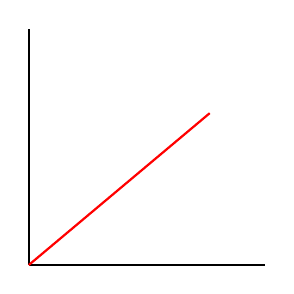
\begin{tikzpicture}
\draw [thick] ( 0,0) -- (3,0);
\draw [thick] ( 0,0) -- (0,3);
\draw [red,thick] ( 0,0) -- (400:3);
\bigangle[blue,dashed]{400}
\end{tikzpicture}
\end{document}
\end{verbatim}

% \includegraphics{https://i.stack.imgur.com/4RO8Y.png}{图片图片}
\end{faq}


\begin{faq}{如何画交换图?}
\end{faq}


\begin{faq}{如何在插入的图(\cs{includegraphics}\Arg{...})的特定位置插入符号或图}

可以使用 overpic 宏包,在 overpic 环境内进行图形绘制,环境内可以使用
latex 自生 picture 环境的绘图语句进行绘制。以下面给出一个例子:

\begin{verbatim}
\documentclass{article}
\usepackage{graphicx}
\usepackage{overpic}
\begin{document}
\begin{overpic}[width=0.8\textwidth
               %,grid,tics=10 % 取消注释可以产生网格线帮助定位,完成后再将其注释。
               ]{1.png}
  \put(35,10){\LaTeX}
  \put(80,0){\includegraphics[width=0.16\textwidth]{1.png}}
\end{overpic}
\end{document}
\end{verbatim}

下面左边是原图,右边是代码处理后的图片:
% \includegraphics{https://images-cdn.shimo.im/VFe2jSxjmoMZpr2B/1.png!thumbnail}
% \includegraphics{https://images-cdn.shimo.im/4qswwF2P4u44JNYB/2.png!thumbnail}

当然还有一种方法可以使用 tikz 宏包,在 tikzpicture
环境引入图片,并在此基础上进行绘图,这样的优点是绘图语句更为丰富,功能更强大。下面举个例子:

\begin{verbatim}
       ![图片](https://images-cdn.shimo.im/LrJDsfrVZIAerfPW/image.png!thumbnail)  ![图片](https://images-cdn.shimo.im/sVlNCmljor0SctYs/image.png!thumbnail)
\end{verbatim}

第一个为原图,第二个是在原图基础上添加一个标号和边.
其中的格线是用来辅助做图的。

\begin{verbatim}
\documentclass{article}
\usepackage{tikz}
\begin{document}
\pgfdeclarelayer{foreground}
\pgfdeclarelayer{background}
\pgfsetlayers{background,main,foreground}
\begin{tikzpicture}
\begin{pgfonlayer}{background}
\path[xshift=-1.24pt,yshift=4pt]      (0,0) node (o) {
  \includegraphics[width=2.8cm]{graph.pdf}};
\end{pgfonlayer}
\begin{pgfonlayer}{foreground}
    \node at (0,0) [label={[label distance=-2mm]40:$u$}]{};
    \draw[step=.5cm,help lines] (-1.4,-1.4) grid (1.4,1.4);
    \coordinate (A) at (0,1.36);
    \coordinate (B) at (0.91,-1.14);
    \fill[color=red] (B) circle (1pt);
    \draw[line width=0.6pt](A)--(B);
\end{pgfonlayer}
\end{tikzpicture}
\end{document}
\end{verbatim}



\section{十一、开发篇-含LaTeX3}

介绍宏开发技巧,宏包和模板类开发的常见问题。
\end{faq}


\begin{faq}{在阅读已有的宏包或者文类时,遇到未知的命令应如何处理}

可以参照胡伟的《LaTeX2e文类和宏包学习手册》中的第四章-命令集注。



\section{十二、常见错误提示}

\begin{itemize}
  \item
    ! LaTeX Error: File `xxx.sty' not found.
    \cs{usepackage}时,引用错误宏包名称或者本机未下载相应的宏包。解决方法为检查拼写,或TeXLive使用tlmgr安装宏包。
  \item
    ! LaTeX Error: File `xxx.cls' not found.
    \cs{documentclass}时,引用错误文类名称或者本机未下载相应的文类。解决方法为检查拼写,或TeXLive使用tlmgr安装文类。
  \item
    ! Undefined control sequence.
    编译遇到不存在的命令(未定义的控制序列)。解决方法为检查拼写,引用相应的宏包,或者定义该命令。
  \item
    ! Missing \{ inserted. 或者 ! Missing \} inserted.
    缺少分组的某个花括号。解决方法为仔细查找上下文对应的花括号。
  \item
    ! Missing \$ inserted.
    缺少数学环境,通常为把数学环境专用的命令用在普通文本模式。
  \item
    ! LaTeX Error: Can be used only in preamble.
    有许多命令只能用于导言区,如果在document
    环境中用了这些命令,将显示上面的错误信息。
  \item
    ! LaTeX Error: Counter too large.
    计数器数值太大,一般是在需要以字母形式显示的计数器其数值超过了26。
  \item
    ! LaTeX Error: \cs{include} cannot be nested.
    在一个已经要用 \cs{include} 引入的文件中又使用了
    \cs{include} 命令。
  \item
    ! LaTeX Error: Missing \verb|\begin{document}|
    这种情况可能是忘了输入 \verb|\begin{document}|,或者是在导言区中有可打印的文本,还有可能是编译中断时在
    aux 等辅助文件中写入错误,对于后者,可以清理辅助文件后重新进行编译。
  \item
    ! LaTeX Error: No counter `xxx' defined.
    调用某计数器,但该计数器并不存在。
  \item
    ! LaTeX Error: No \cs{title} given. 在给出
    \cs{title} 声明之前就使用了 \cs{maketitle} 命令。
  \item
    ! LaTeX Error: Something's wrong--perhaps a missing \cs{item}.
    导致这个问题一般是在列表环境中的文本不是由 \cs{item} 开始的。
  \item
    ! LaTeX Error: There's no line here to end.
    在 \cs{par} 或空行后调用命令 \cs{newline} 或 \verb|\\|。
    这里它们没有任何意义,如果需要额外竖直间距,应使用 \cs{vspace} 命令。
  \item
    ! LaTeX Error: Lonely \cs{item} -- perhaps a missing list enviroment.
    在列表环境外使用了 \cs{item} 命令。
\end{itemize}
\end{faq}



\section{十三、用法惯例}


\begin{faq}{TeX编辑器中的魔法注释}

在TeX中有单行注释命令为\%,其后的文本主要是对源代码进行一些说明,它们会被TeX,LaTeX等排版引擎所忽略。但有些注释对专门的TeX相关编辑器来说,可能用特别的意义。在不同的TeX编辑器中,这魔法注释(magic comments)可能是不同的。 下面是一些例子: * 指定TeX编译器

\begin{verbatim}
TeXStudio,TeXworks, Sublime Text
% !TeX program = xelatex

TeXShop
%!TEX TS-program = xelatex
\end{verbatim}

同理,将 xelatex 变为 pdflatex,就可以强制调用 pdfLaTeX 编译器。
在代码中需要使用ifxetex宏包进行条件判断。 * 指定文档为 utf-8 编码

\begin{verbatim}
TeXworks,TeXStudio, Sublime Text
% !TeX encoding = utf8
\end{verbatim}

Winedt(由于Winedt对编码自动识别能力较弱,使用此注释比较必要,不然要手动设置)

\begin{verbatim}
% !Mode:: "TeX:UTF-8"
或者
% -*- coding: utf-8 -*-

TeXShop
%!TEX encoding = UTF-8 Unicode
\end{verbatim}

\begin{itemize}

\item
  指定主文档
\end{itemize}

\begin{verbatim}
TeXStudio, Sublime Text
% !TeX root = filename
\end{verbatim}

若需要指定上一层次的文件,则应该使用以下命令

\begin{verbatim}
TeXStudio, Sublime Text
% !TeX root = ../main.tex
\end{verbatim}

用两点表示返回上一层次,如果还需要再返回一个层次,则需要

\begin{verbatim}
TeXStudio, Sublime Text
% !TeX root = ../../main.tex
\end{verbatim}

\begin{itemize}

\item
  指定bib处理程序
\end{itemize}

用biber处理bib文件,可在文件头添加如下代码

\begin{verbatim}
TeXStudio
% !TeX TXS-program:bibliography = txs:///biber
\end{verbatim}

将biber改为bibtex,就可指定bibtex处理bib文件。 * 为TeX编译器指定参数

有时在使用某些宏包时我们需要额外调用一些编译参数,例如 minted
宏包需要使用 --shell-escape,这时可用如下魔法注释实现该功能

\begin{verbatim}
TeXStudio
% !TeX TXS-program:compile = txs://xelatex/[--shell-escape]

sublime text - latextools
%!TEX options = --shell-escape

texshop
\end{verbatim}

MathJax是一个JavaScript引擎,用来显示网络上的数学公式。它支持LaTeX、MathML、AsciiMath符号。查阅MathJax支持的LaTeX命令请参考\href{http://http//onemathematicalcat.org/MathJaxDocumentation/TeXSyntax.htm}{http//onemathematicalcat.org/MathJaxDocumentation/TeXSyntax.htm}

\begin{verbatim}
-shell-escape
\end{verbatim}

下面是各种编辑器对魔法注释的支持情况
\textbar{}Encoding\textbar{}Program\textbar{}Root\textbar{}Spellcheck\textbar{}
:----\textbar{}:----\textbar{}:----\textbar{}:----\textbar{}:----\textbar{}
TeXShop\textbar{}x\textbar{}x\textbar{}x\textbar{}x\textbar{}
TeXStudio\textbar{}x\textbar{}x\textbar{}x\textbar{}x\textbar{}
TextMate\textbar{}?\textbar{}x\textbar{}x\textbar{}?\textbar{}
TeXworks\textbar{}x\textbar{}x\textbar{}x\textbar{}x\textbar{}
SublimeText \textbar{}x\textbar{}x\textbar{}x\textbar{}x\textbar{}
VSCode\textbar{}x\textbar{}x\textbar{}?\textbar{}?\textbar{}
Atom\textbar{}o\textbar{}x\textbar{}x\textbar{}o\textbar{} Vim
(vimtex)\textbar{}o\textbar{}x\textbar{}x\textbar{}o\textbar{}
Texpad\textbar{}o\textbar{}o\textbar{}?\textbar{}?\textbar{} 注意:
x:支持特性 o:不支持特性
?:不确定\textbar{}\textbar{}\textbar{}\textbar{}\textbar{}

\begin{itemize}

\item
  其它
\end{itemize}
\end{faq}


\begin{faq}{LaTeX与数学软件(Mathematica,
Maple,Sagemath等)}
\end{faq}


\begin{faq}{LaTeX与公式编辑器}
\end{faq}


\textbf{官网}:http://www.latexstudio.net \textbf{微信公众号}:latex2015
\textbf{QQ 交流群}:91940767

% Copyright (C) 2018 by latexstudio <http://www.latexstudio.net>
%
% This program is free software: you can redistribute it and/or modify
% it under the terms of the GNU General Public License as published by
% the Free Software Foundation, either version 3 of the License, or
% (at your option) any later version.
%
% This program is distributed in the hope that it will be useful,
% but WITHOUT ANY WARRANTY; without even the implied warranty of
% MERCHANTABILITY or FITNESS FOR A PARTICULAR PURPOSE.  See the
% GNU General Public License for more details.
%
% You should have received a copy of the GNU General Public License
% along with this program.  If not, see <http://www.gnu.org/licenses/>.
%

\section{文档编辑}


\faq{\LaTeXTeX{} 教程}{latex-tex-tutorial}
lshort-zh 是一本比较薄的针对中文用户的 \LaTeX{} 入门教程,该教程已在发行版中,用户可以在命令行中执行
\begin{verbatim}
  texdoc lshort-zh
\end{verbatim}
来查阅。 \LaTeX wikibook 是
% \href{https://www.latex-project.org/help/books/}{https://www.latex-project.org/}
\url{https://www.latex-project.org/help/books/} 中列出的 \TeX{} and \LaTeX{} Books 之一,用户可访问
\url{https://en.wikibooks.org/wiki/LaTeX} 进行查阅。
除此之外,用户还可以购买胡伟、刘海洋等编著书籍,这里不再赘述。


\faq{关于 \LaTeX{} 的书籍}{latex-books}
\begin{itemize}
  \item \LaTeX{} 入门,刘海洋, 电子工业出版社;
  \item \LaTeX{2$\varepsilon$} 完全学习手册(第 2 版),胡伟,清华大学出版社;
  \item \LaTeX{} 入门与提高(第二版) ,陈志杰等,高等教育出版社(注:此书出版逾十年,部分内容已经过时);
  \item \LaTeX{} Beginner's Guide, Stefan Kottwit, Packt Publishing.
\end{itemize}


\faq{\LaTeX{} 支持中文有哪些方式,如何选择}{latex-chinese-how-to-choose}
历史上,\LaTeX{} 支持中文的方式包括中西文点点通、天元、CCT、CJK 等。目前流行的方式是使用 \CTeX{} 宏集,详情请见
\url{https://mirrors.tuna.tsinghua.edu.cn/CTAN/language/chinese/ctex/ctex.pdf}


\faq{关于教程,用户比较容易获取的有两个:lshort 和 \LaTeX{} wikibook。}{lshort-latex-wikibook}


\faq{关于\TeX{}, Plain \TeX{} 及相关书籍}{tex-plain-tex-books}


\faq{关于类型的书籍}{kind-related-books}


\faq{关于其他TeX相关事项的书籍}{other-tex-books}


\faq{工具包文档}{package-document}
每个工具包自带的文档是最全面最权威的文档,一般可以通过 texdoc
命令+工具包名的方式找到相应工具包的文档。
一些常用的工具包有不少爱好者写了自己使用过程中的经验,也可以找来看看。


\faq{可免费提供的 \LaTeXTeX{} 书籍}{free-latex-tex-books}
\begin{itemize}
  \item \LaTeX{} 常用数学符号
  \item \LaTeX{} Note 包太雷
  \item 一份不太简短的 \LaTeX{2e} 介绍
  \item \TeX{} Live 指南 2018
\end{itemize}


\faq{获取在线帮助}{gain-online-help}
一般资料可以去 wikibook 上面查询,网址是
\url{https://en.wikibooks.org/wiki/LaTeX}。
提问可以先到 \LaTeX{} Stack Exchange 看看,网址是
\url{https://tex.stackexchange.com/}。


\faq{如何提出问题}{how-to-ask-questions}

在问问题的时候,要先自己尝试,先问自己如何解决,清晰有效的组织自己想问的问题,究竟想表达什么?没有人会为你不知所谓的问题
浪费时间,就算有人愿意理你,也会因为你的问题不清晰甚至完全无效的问题而伤透脑筋,为了自己,也为了别人,建议大家可以参考下
\href{https://www.jianshu.com/p/f96aa7f7bf59}{《提问的艺术》}这篇文字,清晰有效的提出自己的问题。迷你范例(MWE)
是为别人帮助解决你的问题提供最大化便利的有效手段之一。

最后,需要强调的是,我们愿意在我们的能力范围内为你的问题进行讨论,尽全力帮你解决问题,但这并不是我们的义务,应当尊重别人
拒绝提供帮助的权利。另外,在 QQ 群提出问题所使用的代码最好代码粘贴的网站,如
\href{https://paste.ubuntu.com/}{Ubuntu Pastebin}
暂存,避免刷屏,影响效率。


\faq{如何制作一个迷你范例(MWE)}{how-to-make-MWE}
迷你范例即最小工作示例,英文简称 MWE,以下内容摘自刘海洋的《\LaTeX{} 入门》。

最小工作示例就是一个精简到最小长度的、可以说明所需问题的 \TeX{} 源文件。一方面,最小工作示例应该是一个完整的、可以直接
编译的文件,利用示例可以方便地再现遇到的问题,不需要添加额外的代码;另一方面,示例文件应该尽可能地短小(一个典型的 MWE
一般不超过 10 行),不包含额外的文件,也没有与问题无关的文字代码干扰相对错误的分析。完整的 MWE 应当包括如下信息:
\begin{itemize}
  \item 编译环境,至少应当包括使用的操作系统(如 Windows,macOS,Ubuntu)、安装的发行版(如 \CTeX{},\TeX{} Liv
  e,\MacTeX{} )和使用的集成开发环境(IDE)或编辑器(如 WinEdit,TeXstudio,TeXshop)
  \item 完整的编译命令,如使用的排版引擎(如 \LaTeX{},\XeLaTeX{})
  \item 源文件使用的编码,不同的编辑器的默认编码设置不同,没有事先声明可能会造成复现 bug 困难或出现其他 bug
  \item 完整的代码,但应尽量删除与错误无关的部分,即保证代码可以直接运行的前提下,删除所有与错误部分无关的内容和信息,
  足以重现出现的错误信息和问题即可。不要截图!使别人可以直接复制粘贴你的代码到编译器中,直接重现问题,而不是将时间浪费在
  码字上
  \item 编译错误信息,或你发现与预期不符的 PDF 效果
  \item 如使用了模板,还需附上模板的相关信息,如下载链接和使用说明
\end{itemize}


\faq{学习如何撰写 \LaTeX{} 类及工具包}{learn-how-to-write-latex-and-tools}

可以用命令行使用 |texdoc| 查看 clsguide,dtxtut,macros2e;classes,source2e,The TeXBook;expl3,interface3,
l3styleguide,source3(参考自\href{https://www.zhihu.com/question/27017364}{知乎})。以及《\LaTeX{2e}
文类和宏包学习手册》(胡伟,清华大学出版社)。


\faq{MetaFont 和 MetaPost 教程}{metafont-metapost-tutorial}


\faq{在线介绍:\LaTeX{}}{}


\faq{在线介绍:Plain \TeX{}}{}


\faq{如何让参考文献满足国标GB7714-2015样式要求}{how-to-reference-GB}

有两种比较简单的方式。
\begin{itemize}
  \item 利用 biblatex,一个典型示例如下
  \begin{verbatim}
    \documentclass{ctexart}
      \usepackage[backend=biber,style=gb7714-2015]{biblatex}
      \addbibresource{bibfilename.bib}
      \begin{document}
        引用文献\cite{bibkey1,bibkey2}
        \printbibliography
      \end{document}
    \end{verbatim}
  \item 利用 biblatex,一个典型示例如下
  \begin{verbatim}
    \documentclass{ctexart}
      \usepackage{gbt7714}
      \begin{document}
        引用文献\cite{bibkey1,bibkey2}
        \bibliography{bibfilename}
      \end{document}
  \end{verbatim}
\end{itemize}


\faq{专家邮件列表}{}


\faq{Pic\TeX{} 手册}{}


\faq{基于 \TeX{} 系统的教程}{}


\faq{排版教程}{}


\faq{关于 \TeX{} 的 Wiki 书籍}{tex-wiki-books}

\LaTeX{} wikibook 是 \url{https://www.latex-project.org/} 中列出的 \TeX{} and \LaTeX{} Books 之一,用户
可访问 \url{https://en.wikibooks.org/wiki/LaTeX} 进行查阅。


\faq{如何找到\ldots{}符号:}{how-to-find-symbols}
%
%
在 \LaTeX{} 中插入符号主要有两种思路。一种方式是加载符号宏包,利用宏包提供的命令插入符号;而对于 \XeTeX{} 引擎,目前使用的
多为 Unicode 编码的字体,直接加载 Unicode 字体,插入 Unicode 符号也是一种很好的办法。下面分别介绍:
\begin{itemize}
  \item 加载符号宏包:\emph{The Comprehensive LATEX Symbol List} 收录了上万文本或数学符号,在命令行中键入
  \begin{verbatim}
    texdoc symbols-a4
  \end{verbatim}
  即可打开该文档。此外,\url{http://detexify.kirelabs.org/classify.html}提供了手写识别前述文档中所有符号的功能,
  十分便捷,它可直接符号所在宏包。在 macOS 下可以直接使用 detexify 的 app。另外
  \url{https://webdemo.myscript.com/views/main/math.html}可将手写公式转化为 \LaTeX{} 或 MathML 代码
  \item 插入Unicode符号:可以从各种Unicode码表或字符映射表中找到所需要的符号,查出其编码,加载支持该码位的字体,
  直接在编辑器中输入该符号即可。如果符号在源代码编辑器中无法正常显示,还可以使用\LaTeX{}的 |symbol| 命令输入。
  |symbol| 命令的具体用法是
  \begin{verbatim}
    \symbol{<十进制编码>}
    \symbol{"<十六进制编码>}
    \symbol{'<八进制编码>}
    \symbol{`<字符形式(特殊符号须加转义符 \ )>}
  \end{verbatim}
\end{itemize}

如果使用的TeXstudio软件想要查找某个符号,那么还可以拓展以下2个便捷的方式:
\begin{itemize}
  \item 如下图点开1处的符号,再在2处选择符号类型,缩小查找范围,有运算符、关系、箭头、分隔符、Greek、Cyrillic等,再点击需要的符号加入到数学环境中去这样就插入完成了。

  \includegraphics[width=0.9\textwidth]{include/images/5.png}
  \item 也可以手动输入,识别率不是特别高,可能需要多输入几次才会出来。设置如下:向导$\rightarrow$数学助手,手写输入完之后插入即可。

  \includegraphics[width=0.9\textwidth]{include/images/image.png}
\end{itemize}


\faq{如何找到 FAQs}{}


\faq{如何控制章节编号的深度}{how-to-control-section-depth}

\LaTeX{} 标准文档类对章节划分了层级:
\begin{itemize}
  \item 在 article 文档类里 part 为0,section 为1,依此类推;
  \item 在 report/book 文档类里 part 为 $-1$,chapter 为0,section 为1,等等。
\end{itemize}

secnumdepth 计数器控制章节编号的深度,如果章节的层级大于secnumdepth,那么章节的标题、在目录和页眉页脚的标题都不编号(照常生成目录和页眉页脚),
章节计数器也不计数。可以用 |setcounter| 命令设置 secnumdepth 为较大的数使得层级比较深的章节也编号,
如设置为4令 |paragraph| 也编号;或者设置一个较小的数以取消编号,如设置为-1 令 |chapter| 不编号。
后者是生成不编号的章节的一个妙招,免去了手动使用 |addcontentsline| 和 |markboth| 的麻烦。
secnumdepth 计数器在 article 文档类里默认为3(subsubsection一级);在 report 和 book 文档类里默认为2(subsection 一级)。

下面给出一个具体的例子:

\begin{verbatim}
  \documentclass{book}
  \setcounter{secnumdepth}{4}
  \begin{document}
    \part{part}
    \chapter{chapter}
    \section{section}
      \subsection{subsection}
      \subsubsection{subsubsection}
        \paragraph{paragraph}
  \end{document}
\end{verbatim}

控制目录页排版显示深度可以使用 |\setcounter{tocdepth}{2}|,此命令表示显示到三级标题。关于此问题的具体介绍可以参考
\href{https://blog.csdn.net/RobertChenGuangzhi/article/details/50480856}{该网页}。


\faq{如何下载 arXiv 上面的 \TeX{} 源文件}{how-to-download-arxiv-tex}
先访问 arXiv 上面的文章,在右边找到 Downloads $\rightarrow$ Other formats,点击进入下载页,点击 Download source。
将文件下载到本地后,重命名文件,文件后缀名是 .tar.gz。接下来解压缩 .tar.gz 文件,即可获得 \TeX{} 源文件。


%\begin{faq}{windows 系统下用 texstudio 打开中文编写的源文件遇到乱码怎么办}
%
%  最简单的方法是借助 notepad++ 等编辑器将文件转码为 UTF-8。如果没有
%  noteapd++,也可以直接使用 texstudio。这里我们默认文件的编码是 GB2312。
%  首先打开文件,在 texstudio 右下角找到 encoding
%  位置的内容,有时系统显示为 ISO-8859-1。点击那里,进入 More
%  encodings,在列表中点击 GB2312,然后点击按钮 view
%  with。正常来讲,乱码应该都会消失。 接下来,继续进入 More
%  encodings,在列表中点击 UTF-8,然后点击按钮 change to。
%  经过这些操作,源文件就重新变成了 UTF-8 编码。
%\end{faq}
%
%
%\begin{faq}{69.如何在listing抄录环境中显示公式}
%
%  有时对抄录环境中的代码进行说明时,要用显示公式,
%  这时只要进选项texcl设为true即可,或者设置mathescape~选项为true。
%
%  \begin{verbatim}
%  \begin{lstlisting}[
%  numbers=left,
%  upquote=true,
%  basicstyle=\ttfamily,
%  texcl=true,
%  language=Python
%  ]
%  #Generates Graphs $G^{(12)} ---  G^{(17)}$
%  sGL6=['E@QW', 'EHQW', 'E@`w', 'E@]o', 'E@Rw', 'EAMw']
%  GL=[Graph(s) for s in sGL6]
%  \end{lstlisting}
%  \end{verbatim}
%
%  % \begin{figure}
%  % \centering
%  % \includegraphics{https://images-cdn.shimo.im/LttXT6sECbcak9Qi/image.png!thumbnail}
%  % \caption{图片}
%  % \end{figure}
%
%  \begin{verbatim}
%  \begin{lstlisting}[mathescape=true]
%  if foo
%  list= { $S_1,S_2,S_3$ }
%  \end{lstlisting}
%  \end{verbatim}
%\end{faq}
%
%
%\begin{faq}{能不能介绍一下排版试卷的方法与技巧,比如选择题,密封线设置等。}
%
%  \begin{enumerate}
%    \def\labelenumi{\arabic{enumi}.}
%    \setcounter{enumi}{1}
%
%    \item
%    一个文档,如何在不同部分使用不同的页眉页脚
%  \end{enumerate}
%
%  参考 geometry 宏包的自定义命令。大概就是 \cs{newgeometry}\marg{options}
%  和\cs{restoregeometry} 以及 \cs{savegeometry}\marg{name}
%  和loadgeometry\{\}这四个命令了。具体可参见该宏包的说明文档。 3.
%  如何给中文文本加注音符号?
%
%  xpinyin 宏包 4. 在book类文档中边注用什么宏包?边注的宽度能调整吗? 5.
%  如何使用ctex相关类或者宏包制定章节样式,目录样式?
%
%  一言难尽啊 6. 如何给章节标题,目录列表加盒子边框? 7. 如何使用带圈数字?
%
%  \begin{enumerate}
%    \def\labelenumi{\arabic{enumi}.}
%    \setcounter{enumi}{7}
%
%    \item
%    如何改变列表标签样式,行距,缩进等各种相关间距?
%  \end{enumerate}
%
%  enumitem 宏包 9. 换行与换段的区别,有几种方式?
%
%  换行是\ 换段是
%
%  \par
%
%  ,或者空一行
%
%换行与分段最大的区别在于语义上是否形成一段完整的阐述、叙述,多读两遍你写的文字,如果你觉得问题没有叙述完,那么应该用换行,反之则应该用分段。
%\end{faq}
%
%
%\begin{faq}{在使用较早版本的CTeX里面附带的 winedt 出现打不开utf8编码文档的情况,如何处理?}
%
%  使用记事本之类文本编辑器打开,转换编码方式另存一份即可。有时候需要注意BOM问题,一般没啥问题。
%\end{faq}
%
%
%\begin{faq}{如何改变计数器样式为 中文数字 罗马数字 阿拉伯数字 拉丁字母?}
%
%  可以通过重定义命令的方式修改默认的计数器样式,例如:
%
%  \begin{verbatim}
%  \renewcommand{\thechapter}{\Roman{chapter}}
%  \end{verbatim}
%
%  如上指令将章序号计数器改为大写罗马数字计数形式。
%  % \arabic\textbar{}阿拉伯数字\textbar{} :----\textbar{}:----\textbar{}
%  % \alph\textbar{}小写英文字母,数值应小于27\textbar{}
%  % \Alph\textbar{}大写英文字母,数值应小于27\textbar{}
%  % \chinese\textbar{}中文小写数字,需要调用ctex宏包\textbar{}
%  % \roman\textbar{}小写罗马数字\textbar{}
%  % \Roman\textbar{}大写罗马数字\textbar{}
%  % \fnsymbol\textbar{}脚注标识符,数值应小于10\textbar{}
%
%  详情可以参阅刘海洋、胡伟等编写的相应书籍,也可以查阅wiki百科。 2.
%  列表环境 (enumerate/itemize/description)
%  的条目间距太大了,怎么改小一些?
%
%  可以使用 paralist
%  宏包,它提供了一系列压缩了行间距的列表。对应的环境名称分别是
%  compactenum/compactitem/compactdesc ,也可以使用 enumitem
%  宏包修改三个列表环境的格式。 3.
%  列表的条目项内容很短,可以让他们在一行内排版么?
%
%  可以使用 paralist 宏包,这个宏包提供了 inparenum/inparitem/inpardesc
%  环境,可以在行内输出列表内容;也可以带上 inline 选项使用 enumitem
%  宏包,可以使用带*形式的三个列表环境,即在行内输出列表内容。 4. enumerate
%  宏包修改列表标签格式很方便,但是这个宏包和 enumitem
%  宏包冲突,有什么解决办法么?
%
%  如果只是需要使用这种短标签表示方法,利用 enumitem
%  宏包同样能够做到,只需要带上 shortlabels 选项加载 enumitem
%  宏包即可。同时,enumitem
%  宏包提供了自定义短标签名称和格式的宏命令,你也可以自己定义一些有趣的标签形式。
%  5. 如何使用带圈数字作为 enumerate 列表的标签?
%
%  LaTeX 自带一个带圈字符的命令
%  \textcircled,不过,这个命令的排版效果非常差,几乎很少有人会直接使用。带圈数字可以通过unicode字符实现,也可通过
%  pifont 宏包中 \cs{ding} 命令实现(但是只能用到10以内的数字),甚至可以通过
%  tikz 自己绘制一个。使用带圈数字做enumerate的标签,可以通过 enumitem
%  宏包设置。这里给出一个使用 unicode 字符实现带圈数字的方法,并将其应用于
%  enumerate 的标签。
%
%  \begin{verbatim}
%  \documentclass{article}
%  \usepackage{xeCJK,xunicode,calc}
%  \usepackage[shortlabels]{enumitem}
%  \newcommand{\Cnum}[1]{%
%  \ifnum #1<21
%  \edef\a{\the\numexpr #1+9311}
%  \else
%  \ifnum #1<36
%  \edef\a{\the\numexpr #1+12860}
%  \else
%  \ifnum #1<51
%  \edef\a{\the\numexpr #1+12941}
%  \else
%  \PackageError{your package}{Number too large}{}
%  \fi
%  \fi
%  \fi
%  {\CJKfontspec{Noto Serif CJK SC}\fontspec{Noto Serif CJK SC}\symbol\a}}
%  \SetEnumerateShortLabel{o}{\protect\Cnum{\arabic*}}
%  \begin{document}
%  \Cnum{12} \Cnum{32} \Cnum{46}
%
%  \begin{enumerate}[o]
%  \item The first item.
%  \item The second item.
%  \item The Third One.
%  \end{enumerate}
%  \end{document}
%  \end{verbatim}
%\end{faq}
%
%
%\begin{faq}{如何给目录中的章节都带上引导点来连接页码?}
%
%  其实级别较高的章节结构,如 book/report
%  中的chapter和arcticle中的section,是不需要这种引导点来连接页码的,有这种需求的多是受MS
%  Word 的影响。如果一定要这种引导点,可以在导言区增加这样一段代码。
%
%  \begin{verbatim}
%  \makeatletter
%  \def\@bfdottedtocline#1#2#3#4#5{%
%  \ifnum #1>\c@tocdepth \else
%  \vskip \z@ \@plus.2\p@
%  {\leftskip #2\relax \rightskip \@tocrmarg \parfillskip -\rightskip
%  \parindent #2\relax\@afterindenttrue
%  \interlinepenalty\@M
%  \leavevmode \bfseries
%  \@tempdima #3\relax
%  \advance\leftskip \@tempdima \null\nobreak\hskip -\leftskip
%  {#4}\normalfont\nobreak
%  \leaders\hbox{$\m@th
%  \mkern \@dotsep mu\hbox{.}\mkern \@dotsep
%  mu$}\hfill
%  \nobreak
%  \hb@xt@\@pnumwidth{\hfil\normalfont \normalcolor #5}%
%  \par}%
%  \fi}
%  \renewcommand*\l@section{\@bfdottedtocline{0}{0em}{1.5em}}
%  \makeatother
%  \end{verbatim}
%
%  当然,最后一句应根据实际的文档类型来重定义\l@chapter或\l@section.
%\end{faq}
%
%
%\begin{faq}{如何临时切换页面大小?}
%
%  \begin{enumerate}
%    \def\labelenumi{\arabic{enumi}.}
%    \setcounter{enumi}{1}
%
%    \item
%    没有编号的章节标题如何添加到目录里?
%  \end{enumerate}
%
%  使用
%  \begin{verbatim}
%  \addcontentsline{toc}{⟨level⟩}{⟨title⟩}
%  \end{verbatim}
%
%  ;举个例子:
%  \begin{verbatim}
%  \section*{译者序}\addcontentsline{toc}{section}{译者序}
%  \end{verbatim}
%
%  这样在目录中译者序是没有编号的,对应等级是section,标题是译者序
%  参考:《lshort》目录章节 3. 怎样定义 第几页/共几页 的页码样式?
%
%  可以调用末页标签宏包lastpage,并将页码设置如下:
%
%  \begin{verbatim}
%  第 \thepage 页 / 共 \pageref{LastPage} 页
%  \end{verbatim}
%
%  如果不想调用这个宏包,还可以自己DIY,虽然ugly,但是可以达到目的 ):
%  在文档末尾设置一个标签,例如在 \verb|\end{doucument}| 前加一句
%  \verb|\label{AllPage}|,然后将页码设置为:
%
%  \begin{verbatim}
%  第 \thepage 页 / 共 \pageref{AllPage} 页
%  \end{verbatim}
%
%  \begin{enumerate}
%    \def\labelenumi{\arabic{enumi}.}
%    \setcounter{enumi}{3}
%
%    \item
%    超链接如何断行?
%  \end{enumerate}
%
%  先写
%
%  \begin{verbatim}
%  \PassOptionsToPackage{hyphens}{url}
%  \end{verbatim}
%
%  再写
%
%  \begin{verbatim}
%  \usepackage{hyperref}
%  \end{verbatim}
%\end{faq}
%
%
%\begin{faq}{在使用较早版本的CTeX里面附带的winedt出现打不开utf8编码文档的情况,如何处理?}
%
%  使用记事本之类文本编辑器打开,转换编码方式另存一份即可。有时候需要注意BOM问题,一般没啥问题。
%  2. 如何在axmath转换代码到texstudio?
%
%  点击下图中第10个按钮,即可将数学公式转换为LaTeX代码,复制即可。
%  % \includegraphics{https://images-cdn.shimo.im/oMh77ZPr7iIsh2tB/image.png!thumbnail}
%  3.
%  双栏文档中,如何可以让左边先写完,然后再切换到右边,而不是左右一样长?
%
%  如果是采用文档类 twocolumn
%  选项实现的双栏模式,正文的排版就是先将左边排完,再从右边开始排。而采用
%  multicol 宏包的 muticols 环境则是左右两边底部对齐的。 4.
%  如何输入中文破折号?
%
%  输入法输入咯,英文的破折号 --- 用于中文不合适。 5.
%  \cs{input} 和 \cs{include} 有何区别? * \cs{include}
%  在读入文件之前会另起一页。\cs{input}
%  命令纯粹是把文件里的内容插入 * \cs{include}不可用于导言区
%\end{faq}
%
%
%\begin{faq}{subfiles有什么用?}
%
%  \begin{enumerate}
%    \def\labelenumi{\arabic{enumi}.}
%    \setcounter{enumi}{1}
%
%    \item
%    ~如何使用latexmk编译文档?
%    \item
%    定理环境要怎么使用?
%    \item
%    算法环境如何使用?
%    \item
%    在lstlisting环境中如何输出破折号?
%    \item
%    minted里面tab键为什么会输出成\^{}\^{}T,如何解决?
%    \item
%    一段代码粘贴到texstudio里面就没有了缩进,如何解决?
%    \item
%    在LaTeX或Tikz中,能否输入随机且字数随机可控的文字?
%    \item
%    如何输入罗马数字等?
%    \item
%    如何在等号中插入问号?
%  \end{enumerate}
%
%  \begin{verbatim}
%  \stackrel{?}{=}.
%  \end{verbatim}
%\end{faq}
%
%
%\begin{faq}{如何在插入的图片上标记引注?}
%
%  \begin{enumerate}
%    \def\labelenumi{\arabic{enumi}.}
%    \setcounter{enumi}{1}
%
%    \item
%    如何让一个很长很长的字符串(中间不带空格)自动换行?
%    \item
%    \cs{bf} \cs{sf} \cs{it} \cs{sl} 这些命令都很短小,为什么不建议继续使用了?
%    \item
%    如何自动化打包 LaTeX
%    文档发送给别人以确保宏包、字体是完整的,便于他人顺利编译、减少麻烦。
%    \item
%    如何编译网站上下载的他人的模板,一般是不知道对应的编译器应该选择什么,还有编译顺序是什么,希望在提供模板的同时说明应该如何编译。
%    \item
%    我以book文档类为基础新写一个文档类,book文档类的选项会自动适用于我新建的文档类么?
%    \item
%    \cs{def} 和 \cs{newcommand}
%    有什么区别,我创建新命令的时候究竟应该用哪个?
%    \item
%    怎样创建一个带*的命令?
%    \item
%    ~类似 \verb|\macro[<option1>][<option2>]{<arg>}|
%    这样的宏命令,当我只使用一个可选参数时,LaTeX
%    把它看做哪个参数?LaTeX会自动判断么?
%    \item
%    \cs{newcommand}
%    创建的命令,仅有第一个命令可以成为可选参数,如果我想创建具有两个可选参数的命令,应该如何去写?
%    \item
%    有些命令的参数是使用( ) 扩起来的,这类命令是如何定义的?
%    \item
%    我想新建一个带有可选参数的命令,可选参数的缺省值与必选参数值一样,这样的命令如何创建?
%    \item
%    想用minted包写文档,怕别人用不来不会设置-shell --escepe咋办
%    \item
%    .latex如何给整个页面加边框?
%  \end{enumerate}
%\end{faq}

% % Copyright (C) 2018 by latexstudio <http://www.latexstudio.net>
%
% This program is free software: you can redistribute it and/or modify
% it under the terms of the GNU General Public License as published by
% the Free Software Foundation, either version 3 of the License, or
% (at your option) any later version.
%
% This program is distributed in the hope that it will be useful,
% but WITHOUT ANY WARRANTY; without even the implied warranty of
% MERCHANTABILITY or FITNESS FOR A PARTICULAR PURPOSE.  See the
% GNU General Public License for more details.
%
% You should have received a copy of the GNU General Public License
% along with this program.  If not, see <http://www.gnu.org/licenses/>.
%

\section{介绍公式的常见问题。}
%\end{faq}
%
%
%\begin{faq}{\cs{ldots} 与...有什么区别?}
%
%重定义的难度不同、造成的间距也不同。推荐使用 {[}\ldots{}{]}。 见
%\url{https://www.zhihu.com/question/27589739/answer/37255728}
%\end{faq}
%
%
%\begin{faq}{如何让长公式自动断行?}
%
%长公式自动断行要看情况,如果是在行内模式,合理使用空格,一般可以在二元运算符处断行,如果是行间模式,推荐使用align类环境,在需要断行处添加
%\textbackslash{} 手动断行。
%\end{faq}
%
%
%\begin{faq}{公式希腊字符如何加粗?}
%
%希腊字母没有粗体,可以选择合适的数学字体。 可以使用 bm
%宏包将希腊字母加粗。
%\end{faq}
%
%
%\begin{faq}{极限符号下面有两个趋近该怎么写}
%
%直接给出例子:
%
%\begin{verbatim}
%\documentclass{article}
%\begin{document}
%\[ \lim_{n\to\infty\atop m\to\infty} \]
%\end{document}
%\end{verbatim}
%
%或者使用 \cs{substack},代码如下:
%
%\begin{verbatim}
%\documentclass{article}
%\usepackage{amsmath}
%\begin{document}
%\[ \lim_{\substack{n\to\infty\\ m\to\infty}} \]
%\end{document}
%\end{verbatim}
%
%效果如下:
%% \includegraphics{https://images-cdn.shimo.im/FCY4A1SeBIcwBCGT/双重极限.PNG!thumbnail}
%\end{faq}
%
%
%\begin{faq}{怎样在 LaTeX
%  中输入引号}
%
%左引号用 `(键盘1旁边那个键),右引号用 `。双引号也一样,``''。
%中文条件下可以直接用中文引号(这个与编码方式和中文支持方式有关的),会有自动配对(这个和编辑器以及输入法有关的),但是如果需要用到不配对引号的情况,需要使用通用方法。
%\end{faq}
%
%
%\begin{faq}{align环境默认是居中对齐吗?我在使用时,发现公式开始是居中的,后来却一直靠右断对齐,这是什么原因?}
%
%\sout{align 默认靠右对齐,所以通常加 \&
%  符号,让代码左对齐。验证一下以下代码:}
%
%\begin{verbatim}
%\begin{align}
%& \nabla \times H = J,\\
%& \nabla \times E = - \partial _t B,\\
%& \nabla \cdot B = 0.
%\end{align}
%\end{verbatim}
%
%再试试把 \& 去掉什么样。
%align采用的是奇偶对齐的方式,第一列右对齐,第二列左对齐,就这样右左右左依此类推,两列之间用\&分隔。
%\end{faq}
%
%
%\begin{faq}{中英文标点使用规则不是很明白,尤其在公式环境里,字体和间距差别都比较大。怎样才能让正文和公式的标点统一(形状和间隔)?}
%
%详见:
%\url{https://link.zhihu.com/?target=http\%3A//www.moe.gov.cn/ewebeditor/uploadfile/2015/01/13/20150113092346124.pdf}
%在导言区加类似命令可实现全文替换:
%
%\begin{verbatim}
%\catcode`\。=\active\newcommand{。}{. }
%\end{verbatim}
%
%或者使用 xeCJK 宏包的字符映射功能,调用 fullwidth-stop
%这一映射文件,将中文空心句号映射为实心句点:
%
%\begin{verbatim}
%\documentclass{article}
%\usepackage{xeCJK}
%\setCJKmainfont[Mapping= fullwidth-stop]{STSong}
%\begin{document}
%句号。
%\end{document}
%\end{verbatim}
%\end{faq}
%
%
%\begin{faq}{公式如何居左对齐,居右对齐?}
%
%公式居左对齐在基础文档类中由 fleqn
%选项控制,选择该选项后,正文公式均居左对齐,至于居右对齐,嗯,我没见过这么奇怪的格式。
%\end{faq}
%
%
%\begin{faq}{公式之后解释公式符号的文字,通常是 ``符号 ------ 解释''
%  这样的格式,我希望这段文字的格式是按破折号对齐,并且解释文字折行后悬挂缩进,怎样实现这样的格式?}
%
%方法很多,可以列表,可以align等环境。 这里给出一个使用自定义列表的例子:
%
%\begin{verbatim}
%\usepackage{ifthen}
%\newcounter{qlst}
%\newenvironment{EqDesc}[2][式中]{%
%\begin{list}{}
%{%
%\usecounter{qlst}
%\settowidth{\labelwidth}{#1,#2\ --- \ }
%\setlength{\labelsep}{0pt}
%\setlength{\leftmargin}{\labelwidth}
%\setlength{\rightmargin}{0em}
%\setlength{\parsep}{0ex}
%\setlength{\itemsep}{0ex}
%\setlength{\itemindent}{0em}
%\setlength{\listparindent}{0em}
%\renewcommand{\makelabel}[1]{\stepcounter{qlst}\ifthenelse{\value{qlst}>1}{\hfill ##1\ --- \ 
%}{#1,\hfill ##1\ --- \ }}
%}}%
%{\end{list}}%
%\end{verbatim}
%
%EqDesc
%环境有两个参数,第一个为可选参数,是解释公式符号前的引导词,默认是``式中'',第二个参数是样本符号,可以选择一个列表中宽度最大的符号。条目
% \cs{item} 有一个可选参数(实际使用是必选参数),内容是要说明的符号。使用如下:
%
%\begin{verbatim}
%\[ a^2+b^2=c^2 \]
%\begin{EqDesc}[其中]{$a$}
%\item[$a$] 三角形的一条直角边;
%\item[$b$] 三角形的另一条直角边;
%\item[$c$] 三角形的斜边。
%\end{EqDesc}
%\end{verbatim}
%\end{faq}
%
%
%\begin{faq}{行内公式的情况下如何让sum
%  prod这些运算符的上下标在头上和脚下?}
%
%这样处理行内公式的上下标会导致段落行距不整齐,不符合 LaTeX
%的审美。如果彻底放弃审美,可以使用 \cs{limits} 命令,如:
%
%\begin{verbatim}
%$\sum\limits_{i=1}^n \quad
%\prod\limits_\epsilon$
%\end{verbatim}
%\end{faq}
%
%
%\begin{faq}{如何将积分的上限标放在积分号的上下两侧?}
%
%积分号的上下限放置在积分号的右侧是英美国家和 LaTeX
%的排版习惯,通常无需处理。如果你很确定需要按照 ISO 80000-2:2009 或者 GB
%3102.11-93 的规定排版积分号,可以:
%
%\begin{enumerate}
%  \def\labelenumi{\arabic{enumi}.}
%  
%  \item
%  在调用 amsmath 宏包时添加 intlimits 选项;
%  \item
%  \texttt{\textbackslash{}def\textbackslash{}int\{\textbackslash{}intop\}}
%  \item
%  如果使用 unicode-math 宏包,
%\end{enumerate}
%
%\begin{verbatim}
%\removenolimits{%
%\int\iint\iiint\iiiint\oint\oiint\oiiint
%\intclockwise\varointclockwise\ointctrclockwise\sumint
%\intbar\intBar\fint\cirfnint\awint\rppolint
%\scpolint\npolint\pointint\sqint\intlarhk\intx
%\intcap\intcup\upint\lowint
%}
%\end{verbatim}
%\end{faq}
%
%
%\begin{faq}{如何自定义数学运算符,然后让下标放在脚下?}
%
%借助 amsmath 包的
%\cs{DeclareMathOperator*} 命令即可(需要注意加不加*是有区别的)。例如
%
%\begin{verbatim}
%\DeclareMathOperator*{\esssup}{ess\,sup}
%\end{verbatim}
%\end{faq}
%
%
%\begin{faq}{在数学公式中,编辑等式时,每一行需要等号和等号对其,这时使用了\textbackslash{}begin\{displaymath\}
%  \textbackslash{}begin\{split\}环境,但是呢,这些整体都是居中的,我想让式子靠左,怎么实现呢?}
%\end{faq}
%
%
%\begin{faq}{行列式变换过程中,我们一般是在中间的箭头上表示出变换的方式,如何才能在长箭头上打出多行内容?}
%\end{faq}
%
%
%\begin{faq}{如何输出反斜杠?}
%
%\begin{verbatim}
%\textbackslash \verb|\|
%\end{verbatim}
%\end{faq}
%
%
%\begin{faq}{对equation环境下的公式、图片编号按章节、小节进行重新定义}
%\end{faq}
%
%
%

% \input{include/5-bib}
% \section{字体篇}
%
%
%\begin{faq}{LaTeX字体是如何处理的}
%
%LaTeX 2ε目前的字体机制称为``新字体选择机制''(New Font Selection
%Scheme,NFSS)。它将文本字体分为五个互不干扰的属性(数学字体初学者不必过早了解):
%\begin{enumerate}
%  \item
%  
%编码(encoding)。这个属性初学者暂时不必了解。在(pdf)latex和uplatex中,默认的西文编码称为OT1;在xelatex中,默认的编码称为EU2,就是Unicode。
%  \item
%  字族(family)。一套成风格的字型的统称,如cmr、ptm(times)等。\LaTeXe{}
%  预先定义了三个切换字族的命令:\cs{rmfamily}(衬线体)、\cs{sffamily}(无衬线体)、\cs{ttfamily}(等宽体)。
%  \item
%  
%系列(series)。在一般的字体中一般表示字重(weight)。如粗体命令为\cs{bfseries},正常粗细为\cs{mdseries}。
%  \item
%  
%字形(shape)。在同一字族、同一系列下的风格差异,如斜体\cs{slshape}、意大利斜体\cs{itshape}、正体\cs{upshape}、小型大写\cs{scshape}。
%  \item
%  字号(size)。以上四种变化是字型(typeface)的变化,而这是同一字型下不同大小的变化。LaTeX
%  2ε提供了成套的字号命令,如\cs{normalsize}、\cs{small}、\cs{scriptsize} 等。
%\end{enumerate}
%
%中文字体的方面,不同的中文解决方案的处理也有不同,这里就不介绍了。
%\end{faq}
%
%
%\begin{faq}{获取位图字体}
%\end{faq}
%
%
%\begin{faq}{PDF格式图片插入过程中的字形缺失}
%\end{faq}
%
%
%\begin{faq}{为数学排版选择Type
%  1字体}
%\end{faq}
%
%
%\begin{faq}{Type 1字体配置}
%\end{faq}
%
%
%\begin{faq}{切换到T1时字体变得模糊}
%\end{faq}
%
%
%\begin{faq}{由于Ghostscript太旧造成字体模糊}
%\end{faq}
%
%
%\begin{faq}{如何使用斜体}
%
%斜体一般是西文字体用的,在中文中不用斜体。
%
%斜体这个名字比较误导,因为它对应英文的两个名字:倾斜体(slanted,指字形风格大致相同但是倾斜)和意大利体(italic,指字形设计为接近手写的形态,同时也就出现了倾斜)。
%
%两种情况下分别有 \cs{slshape} 和 \cs{itshape} 两个命令,使用例如
%\verb|{\slshape slanted}| 及\verb|{\itshape 
%italic}|;也有把斜体内容作为参数的命令(推荐使用这种),如\textsl{slanted}及\textit{italic}。
%\end{faq}
%
%
%\begin{faq}{如何使用粗体}
%
%\begin{enumerate}
%  \def\labelenumi{\arabic{enumi}.}
%  \item
%  \cs{mathbf}
%  
%  \cs{mathbf}
%  会将数学模式取消再来取用字型,因此它加粗的不是数学符号,而是公式里的一般文字。\cs{mathbf} 
%  只能在公式内部使用:
%\end{enumerate}
%
%\begin{verbatim}
%\documentclass{article}
%\begin{document}
%$\mathbf{equation: f(x,y) = \alpha x^2 + \beta y^2}$
%\end{document}
%\end{verbatim}
%
%效果如下:
%% \includegraphics{https://images-cdn.shimo.im/tmTzWYcpaSUPPQCQ/image.png!thumbnail}
%
%\begin{enumerate}
%  \def\labelenumi{\arabic{enumi}.}
%  \setcounter{enumi}{1}
%  \item
%  \cs{boldmath}
%  
%  \cs{boldmath} 可以将整套数学字体切换为粗体版本,这个命令只能在公式外使用:
%\end{enumerate}
%
%\begin{verbatim}
%\documentclass{article}
%\begin{document}
%\boldmath{$f(x,y) = \alpha x^2 + \beta y^2$}
%\end{document}
%\end{verbatim}
%
%效果如下:
%% \includegraphics{https://images-cdn.shimo.im/FT1utRInpn8FWCZX/image.png!thumbnail}
%
%\begin{enumerate}
%  \def\labelenumi{\arabic{enumi}.}
%  \setcounter{enumi}{2}
%  \item
%  \cs{boldsymbol}
%  
%  amsmath 提供了一个 \cs{boldsymbol} 命令(由调用的 amsbsy
%  宏包提供),用于打破 \cs{boldmath}
%  的限制,在公式内部将一部分符号切换为粗体:
%\end{enumerate}
%
%\begin{verbatim}
%\documentclass{article}
%\usepackage{amsbsy}%或者直接调用常用宏包amsmath
%\begin{document}
%$f(x,y) = \boldsymbol{\alpha x^2 + \beta y^2}$
%\end{document}
%\end{verbatim}
%
%效果如下:
%% \includegraphics{https://images-cdn.shimo.im/FiwJiO2EZeYTf4j7/image.png!thumbnail}
%
%\begin{enumerate}
%  \def\labelenumi{\arabic{enumi}.}
%  \setcounter{enumi}{3}
%  \item
%  \cs{bm}
%\end{enumerate}
%
%\begin{verbatim}
%\documentclass{article}
%\usepackage{bm}
%\begin{document}
%$\sum x_i y_i$,
%$\bm{\sum x_i y_i}$,
%${\bm \sum}{\bm x_i}{\bm y_i}$.
%\end{document}
%\end{verbatim}
%
%效果如下:
%% \includegraphics{https://images-cdn.shimo.im/yKpDot5b9oUc6ww3/image.png!thumbnail}
%
%\begin{enumerate}
%  \def\labelenumi{\arabic{enumi}.}
%  \setcounter{enumi}{4}
%  \item
%  \cs{pmb}
%  
%  需使用 amamath 宏包。
%  \item
%  \textbf
%  文本加粗
%\end{enumerate}
%
%\begin{verbatim}
%\documentclass{article}
%\begin{document}
%\textbf{equation: $f(x,y)=\alpha x^2+\beta y^2$}
%\end{document}
%\end{verbatim}
%
%效果如下:
%% \includegraphics{https://images-cdn.shimo.im/ZFmJXLZAIGQKq0VQ/image.png!thumbnail}
%
%\begin{enumerate}
%  \def\labelenumi{\arabic{enumi}.}
%  \setcounter{enumi}{6}
%  
%  \item
%  \cs{bfseries}
%  \cs{bfseries} 影响之后所有的字符,如果想让它在局部生效,需使用花括号分组:
%\end{enumerate}
%
%\begin{verbatim}
%\documentclass{article}
%\begin{document}
%{\bfseries equation: $f(x,y) = \alpha x^2 + \beta y^2$}\\
%equation: $f(x,y) = \alpha x^2 + \beta y^2$.\\
%\bfseries equation: $f(x,y) = \alpha x^2 + \beta y^2$\\
%equation: $f(x,y) = \alpha x^2 + \beta y^2$.\\
%\end{document}
%\end{verbatim}
%
%效果如下:
%% \includegraphics{https://images-cdn.shimo.im/rafHmr9a7JYYebWs/image.png!thumbnail}
%参考: Ishort-zh-cn LaTeX入门,刘海洋。
%\url{http://blog.sina.com.cn/s/blog_5e16f1770100nqwx.html}
%\end{faq}
%
%
%\begin{faq}{如何设置文档字体为本机已安装字体?}
%\end{faq}
%
%
%\begin{faq}{如何通过字体文件名来调用未安装本机字体?}
%\end{faq}
%
%
%\begin{faq}{字体大小经常出现警告,该引用什么宏包解决?}
%\end{faq}
%
%
%\begin{faq}{有些特殊文字怎么加入Latex文档,例如symbol\{"ff0e\}编译后为空白}
%\end{faq}
%
%
%\begin{faq}{如何查看字体和行间距,然后怎样修改}
%\end{faq}
%
%
%\begin{faq}{字体相对大小指令}
%
%\cs{small} 等命令对应的字体大小与文章 \cs{documentlcass} 中指定的字体有关,对应
%10, 11, 12pt 三种全局字体大小的情况如下表所示, 指令 10pt 11pt 12pt
%% \tiny                           5 6 6
%% \scriptsize                 7 8 8
%% \footnotesize            8 9 10
%% \small                        9 10 10.95
%% \normalsize              10 10.95 12
%% \large                       12 12 14.4
%% \Large                      14.4 14.4 17.28
%% \LARGE                    17.28 17.28 20.74
%% \huge                       20.74 20.74 24.88
%% \Huge                      24.88 24.88 24.88
%\end{faq}
%
%
%\begin{faq}{在latex公式中如何将某一个字母或者希腊符号设置成某一个字体?}
%\end{faq}
%
%
%

% \input{include/7-figure}
% \section{表格篇}
%
%
%\begin{faq}{如何指定表格的总宽度}
%
%可以看看tabularx、tabu等宏包。
%\end{faq}
%
%
%\begin{faq}{指定列宽度的表格如何使单元格内容居中}
%
%指定宽度的表格列一般采用 p\{\}
%形式的列格式,这种列格式下,表格内容是两端对齐的,如果想使其成为居中对齐需要借助
%array 宏包提供的功能,示例如下:
%
%\begin{verbatim}
%\begin{tabular}{c|>{\centering\arraybackslash}p{4cm}}
%\hline
%1  &  3.530  \\
%2  &  456.0  \\
%3  &  78.945 \\
%4  &  3.65   \\
%\hline
%\end{tabular}
%\end{verbatim}
%
%而 \verb|>{}p{}|
%这样的格式在文档的应用过程中是非常不方便的,array 宏包同时提供了
%\cs{newcolumntype} 宏命令可以将其定义为一个较为简短的格式,如:
%
%\begin{verbatim}
%\newcolumntype{z}[1]{>{\centering\arraybackslash}p{#1}}
%\end{verbatim}
%
%从而可以在正文中使用
%
%\begin{verbatim}
%\begin{tabular}{c|z{4cm}}
%\hline
%
%1  &  3.530  \\
%2  &  456.0  \\
%3  &  78.945 \\
%4  &  3.65   \\
%\hline
%\end{tabular}
%\end{verbatim}
%
%类似的,采用 \cs{raggedright} 或
%\cs{raggedleft} 替换\cs{centering} 可以使得单元格内容变成左对齐或右对齐。
%\end{faq}
%
%
%\begin{faq}{tabularx 中的 X
%  列格式如何居中对齐}
%
%同样采用 array 宏包的 \verb|>|\marg{format} 方法,并利用
%\cs{newcolumntype} 定义新的列格式,如:
%
%\begin{verbatim}
%\usepackage{array,tabularx}  % this line in preamble
%\newcolumntype{Z}{>{\centering\arraybackslash}X} % this line in preamble
%\begin{tabularx}{\linewidth}{ZZ}
%\hline
%
%1  &  3.530  \\
%2  &  456.0  \\
%3  &  78.945 \\
%4  &  3.65   \\
%\hline
%\end{tabularx}
%\end{verbatim}
%\end{faq}
%
%
%\begin{faq}{tabularx 中的 X
%  列格式,当单元格内容发生换行时,如何使同一行其他列的单元格垂直居中对齐?}
%
%对于指定宽度的表格列格式
%p\{\},单元格内一旦进行换行,该单元格同一行内其他列的单元格内容均为垂直方向上顶端对齐,我们可以使用
%array 宏包,以 m\{\} 列格式或者 b\{\} 列格式 替代 p\{\}
%格式即可实现垂直居中对齐或垂直底部对齐。对于 tabularx 中的 X
%列格式,也是采用同样的思路实现,只是这里需要对
%\cs{tabularxcolumn} 宏进行重定义如下:
%
%\begin{verbatim}
%\usepackage{array,tabularx}   % this line in preamble
%\renewcommand{\tabularxcolumn}[1]{m{#1}}  % this line in preamble
%\end{verbatim}
%
%以上则将同行的其他列单元格设置为垂直居中对齐。显然的,垂直底部对齐的设置方法是将重定义宏命令中的
%m\{\#1\} 替换为 b\{\#1\} 即可。
%\end{faq}
%
%
%\begin{faq}{booktabs的三线表,竖线为什么是不连续的?}
%
%宏包的作者为表格线的前后都增加了额外的sep,而且,宏包的作者认为三线表是不应该有竖线的。当然,如果你一定想要使用竖线,不妨以下面两个命令将表格线前后的sep设置为0pt。
%
%\begin{verbatim}
%\usepackage{booktabs} % this line in preamble
%\setlength{\belowrulesep}{0pt}
%\setlength{\aboverulesep}{0pt}
%\end{verbatim}
%\end{faq}
%
%
%\begin{faq}{表格的一列全是公式,有什么办法能输入简单些?}
%
%可以使用 array 宏包,\verb|>{}| 与\verb|<{}|
%可以为一列数据前后加上特定的宏命令。在一列数据前后均加上 \verb|$| 则把这列数据放入数学模式中,举例如下:
%\begin{verbatim}
%\usepackage{array} % this line in preamble
%\begin{tabular}{>{$}c<{$} c}
%\hline
%\multicolumn{1}{c}{function} & value \\
%g(x)                         & 3.65  \\
%f(x)                         & 2.58  \\
%\sin(x)                      & 14.7  \\
%\hline
%\end{tabular}
%\end{verbatim}
%
%第一列数据省去了输入数学模式起止符号 \verb|$| 的痛苦。对于不需要放入数学模式的单元格,比如表头,需要用 
%\verb|\multicolumn{1}{c}{xxx}| 的方式来保护一下,重新指定对齐方式。
%\end{faq}
%
%
%\begin{faq}{我的表格单元格内容是一个列表环境 
%(enumerate/itemize),它和表格横线之间间距好大啊,怎么能把这些间距去掉?}
%
%把列表环境放入到 minipage 环境中即可,即使表格列格式采用的是p{<width>}格式。
%\end{faq}
%
%
%\begin{faq}{如果想让表格中数字小数点对齐要怎么做}
%
%可以借助 @ 的功能,如
%
%\begin{verbatim}
%\begin{tabular}{r@{.}l}
%\hline
%1 & 0 \\
%23 & 1 \\
%\hline
%\end{tabular}
%\end{verbatim}
%
%或者借助 warpcol 宏包提供的功能,如
%\begin{verbatim}
%\documentclass{article}
%\usepackage{warpcol}
%\begin{document}
%\begin{tabular}{P{3.1}P{-2.1}}
%\hline
%\multicolumn{1}{c}{Label 1} & \multicolumn{1}{c}{Label 2} \\
%\hline
%123.4 & -12.3 \\
%12.3 & 12.3 \\
%1.2 & 1.2 \\
%\hline
%\end{tabular}
%\end{document}
%\end{verbatim}
%
%还可以借助 array 和 dcolumn 的配合,如
%
%\begin{verbatim}
%\documentclass{article}
%\usepackage{array,dcolumn}
%\newcolumntype{d}[1]{D{.}{.}{#1}}
%\begin{document}
%\begin{tabular}{cd{3}}
%\hline
%1 & 3.14 \\
%2 & 27.12 \\
%3 & 78.095 \\
%\hline
%\end{tabular}
%\end{document}
%\end{verbatim}
%
%
%还可以借助 array 和 dcolumn 的配合,如
%
%\begin{verbatim}
%\documentclass{article}
%\usepackage{array,dcolumn}
%\newcolumntype{d}[1]{D{.}{.}{#1}}
%\begin{document}
%\begin{tabular}{cd{3}}
%\hline
%1 & 3.14 \\
%2 & 27.12 \\
%3 & 78.095 \\
%\hline
%\end{tabular}
%\end{document}
%\end{verbatim}
%\end{faq}
%
%
%\begin{faq}{表格竖排}
%
%\begin{verbatim}
%\documentclass{ctexart}
%\usepackage[usestackEOL]{stackengine}
%
%\begin{document}
%
%\setlength\normalbaselineskip{11pt}
%\strutlongstacks{T}
%\begin{tabular}{|c|c|c|}
%\hline
%Foo bar & {\Centerstack{ 这 \\ 一 \\ 列 \\ 竖 \\ 排 }} & Foo bar \\
%\hline
%\end{tabular}
%
%\end{document}
%\end{verbatim}
%\end{faq}
%
%
%\begin{faq}{跨页长表格}
%
%\begin{verbatim}
%\usepackage{longtable}
%\end{verbatim}
%
%,做好对长表格跨页时的设置
%\end{faq}
%
%
%\begin{faq}{双栏中表格过大怎么调整?}
%
%\begin{itemize}
%  
%  \item
%  方法一:用 graphicx 宏包提供的 \cs{resizebox} 命令:
%\end{itemize}
%
%\begin{verbatim}
%\resizebox{width}{height}{function}
%\end{verbatim}
%
%resizebox 会放缩 function 中的内容到 width 宽度、height
%高度。需要注意的是,同时指定宽度和高度,一般会导致缩放的内容变形,你也可以指定其中一项,\sout{另一个用!占位,}这样系统会自适应另一个参数,即相当于scale命令。
%* 方法二:用 \texttt{table*} 取代 table 环境,针对的是单栏表格。 *
%方法三:将表格中的字体缩小。 * 方法四:使用横排:使用 rotating 宏包
%\end{faq}
%
%
%\begin{faq}{如何制作列数可变的表格,例如试卷的计分表?}
%
%主要是使用 makecell 和 interfaces-makecell 宏包。下面给出一个 MWE。
%
%\begin{verbatim}
%\documentclass{standalone}
%\usepackage{ctex,calc,makecell,interfaces-makecell,CJKnumb,tabularx,multirow}
%
%\newcounter{TotalPart}
%\newcounter{SubColumn}
%\newcounter{EmptyColumn}
%
%\setcounter{TotalPart}{1}
%
%% 计分表制作
%\newcommand{\ScoreTable}{
%\setcounter{SubColumn}{\value{TotalPart}+2}
%\setcounter{EmptyColumn}{\value{TotalPart}+4}
%\begin{tabularx}{\textwidth}{|*{\theSubColumn}{X<{\centering}|}*{3}{c|}}
%\hline
%\multicolumn{\theSubColumn}{|c|}{\multirow{2}{*}{试卷卷面成绩}}
%& \multicolumn{1}{c|}{\multirow{3}{3em}{课程考核成绩占~\%}}
%& \multicolumn{1}{c|}{\multirow{3}{3em}{平时成绩占\,\%}}
%& \multicolumn{1}{c|}{\multirow{3}{3em}{课程考核成绩}}
%\\
%\multicolumn{\theSubColumn}{|c|}{}
%& & &
%\\
%\cline{1-\theSubColumn}
%\hfill 题 \hfill 号 \hfill~
%& \repeatcell{\theTotalPart}{text=\CJKnumber{\column}}
%& \hfill 小 \hfill 计 \hfill~
%& & &
%\\
%\hline
%\hfill 得 \hfill 分 \hfill~
%& \eline{\theEmptyColumn}
%\\
%\hline
%\end{tabularx}
%}
%
%\begin{document}
%
%\ScoreTable
%
%\end{document}
%\end{verbatim}
%
%CJKnumb 宏包是为了把阿拉伯数字转换为小写汉字序号。 calc
%宏包是为了做四则运算。 tabularx 宏包是为了做列宽自动扩展的表格。
%multirow 宏包是为了合并单元格。 makecell 是制作表格。
%interfaces-makecell
%宏包提供了一系列命令,使得制作可变表格称为可能,同时简化了表格制作。
%\end{faq}
%
%
%\begin{faq}{如何固定表格的总宽度?}
%
%使用 tabular* 环境或 tabularx
%宏包提供的同名环境即可固定表格的总宽度,宏包 tabu
%功能更为强大,用法也更为复杂,可参见相应宏包文档说明。
%\end{faq}
%
%
%\begin{faq}{表格在单元格内如何换行?}
%
%可以通过限制列宽实现,例如下面的例子
%
%\begin{verbatim}
%\begin{tabular}{|c|c|m{50mm}|}%这里用m则必须调用array宏包
%\hline
%a & b & \LaTeX{}表格固定列宽自动换行自动换行自动换行自动换行自动换行\\
%\hline
%a & b & \LaTeX{}表格固定列宽自动换行自动换行自动换行自动换行自动换行\\
%\hline
%a & b & \LaTeX{}表格固定列宽自动换行自动换行自动换行自动换行自动换行\\
%\hline
%\end{tabular}
%\end{verbatim}
%\end{faq}
%
%
%\begin{faq}{如何插入子图/表,各自分别带子标题,不带子标题?}
%
%可参见并列图形、并列子图的排列
%\end{faq}
%
%
%\begin{faq}{如何减小表格,插图,公式,列表等前后空白?}
%
%表格、插图、公式、列表的前后空白很多是由于不良的文本结构引起的,比如太短篇幅的正文,接连几级标题之间没有正文内容,甚至标题之间只有插图和表格等浮动体而没有任何说明的正文,这些都是不好的行文习惯,应杜绝这样的行文方式。此外,一些不良的代码写法也会引入较大的空白,如:
%
%\begin{verbatim}
%\begin{center}
%\begin{figure}
%...
%\end{figure}
%\end{center}
%\end{verbatim}
%
%或者
%
%\begin{verbatim}
%\begin{figure}
%\begin{center}
%\includegraphics{x.pdf}
%\caption{the title}
%\end{center}
%\end{figure}
%\end{verbatim}
%
%而应该采用的方式是:
%
%\begin{verbatim}
%\begin{figure}
%\centering
%\includegraphics{x.pdf}
%\caption{the title}
%\end{figure}
%\end{verbatim}
%
%这是因为 center 环境本身就是一个 list
%列表环境,其与上下文之间就有垂直间距,加上figure
%浮动体与正文之间的间距,插图与正文之间的间距自然就变大了。
%\end{faq}
%
%
%\begin{faq}{表格如何分页?}
%
%这个问题可见跨页长表格。
%\end{faq}
%
%
%\begin{faq}{表格怎样可以旋转90度?}
%
%希望旋转90度的表格多半是由于过宽而需要进行横排,这里一个方法是使用
%rotating 宏包,使用方法非常简单,用 sidewaytable 替代 table
%即可,但这种表格不能实现跨页长表格(当然又宽又长的表格确实很少见);另一个方法是使用lscape
%宏包提供的 landscape
%环境,进入横排状态,在其中使用相应的环境即可,这种方法可以实现跨页表格,但进入和退出landscape环境时总是会新开一页再进行排版,因此,在其之前的页面可能会留有大量的空白。两种方法各有利弊,可以根据实际需要进行选择。
%\end{faq}
%
%
%\begin{faq}{如何使用图表目录?}
%
%\listoftables
%\listoffigures
%\end{faq}
%
%
%\begin{faq}{图表如何使用双语标题}
%
%使用 bicaption 宏包或 ccaption 宏包。
%\end{faq}
%
%
%\begin{faq}{如何产生表格的竖线,在模板的三线表中产生竖线?}
%
%竖线的产生与否与表格的环境无关,在定义表格列时以 \textbar{}
%分隔列格式即可产生竖线。
%
%\begin{tabular}{l|c|r|}
%  ...
%\end{tabular}
%\end{faq}
%
%
%\begin{faq}{如何在长表格\{longtable\}环境中设置文字自动换行或者固定列宽?}
%\end{faq}
%
%
%\begin{faq}{如何实现表格的奇偶行不同的颜色,长表格也要适用。}
%\end{faq}
%
%
%\begin{faq}{如何使表格单元的左对齐?}
%
%不知道这个问题是啥意思。。。
%\end{faq}
%
%
%\begin{faq}{表格中如何划对角线?}
%
%有宏包 slashbox 或 diagbox 可以制作表格对角线,不过slashbox
%由于没有明确的自由许可信息,已经不为 TeXLive
%所收录了。一个好消息是:diagbox
%有中文版的说明文档,作者的说明总比这里的说明更为准确,直接查阅宏包文档是更好的选择。
%\end{faq}
%
%
%

% \section{Beamer篇}
%
%
%\begin{faq}{129.隐藏导航栏}
%
%Beamer
%自带的导航符号看起来很不错,但是实际上使用的并不多,为了让文稿的显示面积增加,减少干扰元素,我们可以隐藏下方的导航栏符号,两个方法如下:
%
%\begin{verbatim}
%\setbeamertemplate{navigation symbols}{}
%\beamertemplatenavigationsymbolsempty % both ok
%\end{verbatim}
%
%如果需要去掉下方 title,Author 等信息的话,可以用
%
%\begin{verbatim}
%\setbeamertemplate{footline}
%\end{verbatim}
%\end{faq}
%
%
%\begin{faq}{向 Beamer
%  中添加参考文献}
%
%我们可以使用下面的命令添加参考文献,最好放在 `appendix' 后面。
%
%\begin{verbatim}
%\begin{frame}[allowframebreaks]{References}
%\def\newblock{}
%\bibliographystyle{plain}
%\bibliography{mybib}
%\end{frame}
%\end{verbatim}
%\end{faq}
%
%
%\begin{faq}{每节显示目录}
%
%在我们做一个比较长的报告时,我们可能会想在每一节添加一个目录,让听众清楚内容讲到哪了,我们可以在导言区添加如下的命令。
%
%\begin{verbatim}
%\setbeamerfont{myTOC}{series=\bfseries,size=\Large}
%\AtBeginSection[]{\frame{\frametitle{Outline}%
%\usebeamerfont{myTOC}\tableofcontents[current]}}
%\end{verbatim}
%
%为了得到节的标题信息,我们会在帧与帧之间添加
%`\textbackslash{}section{[}short\_title{]}\{long\_title\}', 其中
%short\_title 是短标题,用于 ``页眉''
%信息(header)显示。如果你不想要显示每帧的页眉信息(header),可以使用下面的命令。
%
%\begin{verbatim}
%\setbeamertemplate{headline}{}
%\end{verbatim}
%\end{faq}
%
%
%\begin{faq}{多栏显示}
%
%有时候我们有图需要并排摆放,一个好方法是使用分栏,尤其是当两个图不同的高度的时候,然后在每一栏插入我们需要的图片。代码如下:
%
%\begin{verbatim}
%\begin{columns}[c] % Columns centered vertically.
%\column{5.5cm}     % Adjust column width to taste.
%\includegraphics ...
%\column{5cm}
%\includegraphics ...
%\end{columns}
%\end{verbatim}
%\end{faq}
%
%
%\begin{faq}{添加 LOGO}
%
%在右下方添加 logo,直接用系统默认的命令就可以。
%
%\begin{verbatim}
%\logo{\includegraphics[width=0.08\textwidth]{logo500}}
%\end{verbatim}
%
%如果需要在右上方添加 logo,可以用 TikZ 命令(需要用到 tikz 宏包)在
%Frametitle 上添加。
%
%\begin{verbatim}
%\addtobeamertemplate{frametitle}{}{%
%\begin{tikzpicture}[remember picture,overlay]
%\node[anchor=north east,yshift=2pt] at (current page.north east) 
%{\includegraphics[width=0.09\textwidth]{logo500}};
%\end{tikzpicture}}
%\end{verbatim}
%\end{faq}
%
%
%\begin{faq}{想在 beamer 中新建一个包含 frame 的环境
%  question,该怎么做?}
%
%直接给代码
%
%\begin{verbatim}
%\newenvironment{question}
%{\begin{frame}[environment=question,fragile]
%\begin{theorem}
%}
%{\end{theorem}
%\end{frame}
%}
%\end{verbatim}
%\end{faq}
%
%
%\begin{faq}{如何在默认模板的基础上,定制自己的beamer模板}
%\end{faq}
%
%
%\begin{faq}{如何更改beamer中logo的位置,在使用default的模板和主题下,使用\cs{logo},发现不能更改logo所在位置}
%\end{faq}
%
%
%

% \section{绘图篇}
%
%
%\begin{faq}{如何利用Tikz画超过360º的角,并做好标注}
%
%下面解答来自\url{https://tex.stackexchange.com/questions/60295/drawing-angles-greater-than-360\%C2\%BA-intikz}
%
%\begin{verbatim}
%\documentclass[11pt]{scrartcl}
%\usepackage{tikz}
%\usetikzlibrary{arrows}
%\begin{document}
%\newcommand\bigangle[2][]{%
%\draw[->,domain=0:#2,variable=\t,samples=200,>=latex,#1]
%plot ({(\t+#2)*cos(\t)/(#2)},
%{(\t+#2)*sin(\t)/(#2)}) node[right=.5cm] {$#2^\circ$}
%;}
%\begin{tikzpicture}
%\draw [thick] ( 0,0) -- (3,0);
%\draw [thick] ( 0,0) -- (0,3);
%\draw [red,thick] ( 0,0) -- (400:3);
%\bigangle[blue,dashed]{400}
%\end{tikzpicture}
%\end{document}
%\end{verbatim}
%
%% \includegraphics{https://i.stack.imgur.com/4RO8Y.png}{图片图片}
%\end{faq}
%
%
%\begin{faq}{如何画交换图?}
%\end{faq}
%
%
%\begin{faq}{如何在插入的图(\cs{includegraphics}\Arg{...})的特定位置插入符号或图}
%
%可以使用 overpic 宏包,在 overpic 环境内进行图形绘制,环境内可以使用
%latex 自生 picture 环境的绘图语句进行绘制。以下面给出一个例子:
%
%\begin{verbatim}
%\documentclass{article}
%\usepackage{graphicx}
%\usepackage{overpic}
%\begin{document}
%\begin{overpic}[width=0.8\textwidth
%%,grid,tics=10 % 取消注释可以产生网格线帮助定位,完成后再将其注释。
%]{1.png}
%\put(35,10){\LaTeX}
%\put(80,0){\includegraphics[width=0.16\textwidth]{1.png}}
%\end{overpic}
%\end{document}
%\end{verbatim}
%
%下面左边是原图,右边是代码处理后的图片:
%% \includegraphics{https://images-cdn.shimo.im/VFe2jSxjmoMZpr2B/1.png!thumbnail}
%% \includegraphics{https://images-cdn.shimo.im/4qswwF2P4u44JNYB/2.png!thumbnail}
%
%当然还有一种方法可以使用 tikz 宏包,在 tikzpicture
%环境引入图片,并在此基础上进行绘图,这样的优点是绘图语句更为丰富,功能更强大。下面举个例子:
%
%\begin{verbatim}
%![图片](https://images-cdn.shimo.im/LrJDsfrVZIAerfPW/image.png!thumbnail)  
%![图片](https://images-cdn.shimo.im/sVlNCmljor0SctYs/image.png!thumbnail)
%\end{verbatim}
%
%第一个为原图,第二个是在原图基础上添加一个标号和边.
%其中的格线是用来辅助做图的。
%
%\begin{verbatim}
%\documentclass{article}
%\usepackage{tikz}
%\begin{document}
%\pgfdeclarelayer{foreground}
%\pgfdeclarelayer{background}
%\pgfsetlayers{background,main,foreground}
%\begin{tikzpicture}
%\begin{pgfonlayer}{background}
%\path[xshift=-1.24pt,yshift=4pt]      (0,0) node (o) {
%\includegraphics[width=2.8cm]{graph.pdf}};
%\end{pgfonlayer}
%\begin{pgfonlayer}{foreground}
%\node at (0,0) [label={[label distance=-2mm]40:$u$}]{};
%\draw[step=.5cm,help lines] (-1.4,-1.4) grid (1.4,1.4);
%\coordinate (A) at (0,1.36);
%\coordinate (B) at (0.91,-1.14);
%\fill[color=red] (B) circle (1pt);
%\draw[line width=0.6pt](A)--(B);
%\end{pgfonlayer}
%\end{tikzpicture}
%\end{document}
%\end{verbatim}
%
%
%

% % Copyright (C) 2018 by latexstudio <http://www.latexstudio.net>
%
% This program is free software: you can redistribute it and/or modify
% it under the terms of the GNU General Public License as published by
% the Free Software Foundation, either version 3 of the License, or
% (at your option) any later version.
%
% This program is distributed in the hope that it will be useful,
% but WITHOUT ANY WARRANTY; without even the implied warranty of
% MERCHANTABILITY or FITNESS FOR A PARTICULAR PURPOSE.  See the
% GNU General Public License for more details.
%
% You should have received a copy of the GNU General Public License
% along with this program.  If not, see <http://www.gnu.org/licenses/>.
%

\section{开发篇(含 \LaTeX3)}
%
%介绍宏开发技巧,宏包和模板类开发的常见问题。
%\end{faq}
%
%
%\begin{faq}{在阅读已有的宏包或者文类时,遇到未知的命令应如何处理}
%
%可以参照胡伟的《LaTeX2e文类和宏包学习手册》中的第四章-命令集注。
%
%
%

% \section{常见错误提示}
%
%\begin{itemize}
%  \item
%  ! LaTeX Error: File `xxx.sty' not found.
%  \cs{usepackage}时,引用错误宏包名称或者本机未下载相应的宏包。解决方法为检查拼写,或TeXLive使用tlmgr安装宏包。
%  \item
%  ! LaTeX Error: File `xxx.cls' not found.
%  \cs{documentclass}时,引用错误文类名称或者本机未下载相应的文类。解决方法为检查拼写,或TeXLive使用tlmgr安装文类。
%  \item
%  ! Undefined control sequence.
%  编译遇到不存在的命令(未定义的控制序列)。解决方法为检查拼写,引用相应的宏包,或者定义该命令。
%  \item
%  ! Missing \{ inserted. 或者 ! Missing \} inserted.
%  缺少分组的某个花括号。解决方法为仔细查找上下文对应的花括号。
%  \item
%  ! Missing \$ inserted.
%  缺少数学环境,通常为把数学环境专用的命令用在普通文本模式。
%  \item
%  ! LaTeX Error: Can be used only in preamble.
%  有许多命令只能用于导言区,如果在document
%  环境中用了这些命令,将显示上面的错误信息。
%  \item
%  ! LaTeX Error: Counter too large.
%  计数器数值太大,一般是在需要以字母形式显示的计数器其数值超过了26。
%  \item
%  ! LaTeX Error: \cs{include} cannot be nested.
%  在一个已经要用 \cs{include} 引入的文件中又使用了
%  \cs{include} 命令。
%  \item
%  ! LaTeX Error: Missing \verb|\begin{document}|
%  这种情况可能是忘了输入 \verb|\begin{document}|,或者是在导言区中有可打印的文本,还有可能是编译中断时在
%  aux 等辅助文件中写入错误,对于后者,可以清理辅助文件后重新进行编译。
%  \item
%  ! LaTeX Error: No counter `xxx' defined.
%  调用某计数器,但该计数器并不存在。
%  \item
%  ! LaTeX Error: No \cs{title} given. 在给出
%  \cs{title} 声明之前就使用了 \cs{maketitle} 命令。
%  \item
%  ! LaTeX Error: Something's wrong--perhaps a missing \cs{item}.
%  导致这个问题一般是在列表环境中的文本不是由 \cs{item} 开始的。
%  \item
%  ! LaTeX Error: There's no line here to end.
%  在 \cs{par} 或空行后调用命令 \cs{newline} 或 \verb|\\|。
%  这里它们没有任何意义,如果需要额外竖直间距,应使用 \cs{vspace} 命令。
%  \item
%  ! LaTeX Error: Lonely \cs{item} -- perhaps a missing list enviroment.
%  在列表环境外使用了 \cs{item} 命令。
%\end{itemize}
%\end{faq}
%
%
%


\end{document}
